\documentclass[]{article}
\usepackage{lmodern}
\usepackage{amssymb,amsmath}
\usepackage{ifxetex,ifluatex}
\usepackage{fixltx2e} % provides \textsubscript
\ifnum 0\ifxetex 1\fi\ifluatex 1\fi=0 % if pdftex
  \usepackage[T1]{fontenc}
  \usepackage[utf8]{inputenc}
\else % if luatex or xelatex
  \ifxetex
    \usepackage{mathspec}
    \usepackage{xltxtra,xunicode}
  \else
    \usepackage{fontspec}
  \fi
  \defaultfontfeatures{Mapping=tex-text,Scale=MatchLowercase}
  \newcommand{\euro}{€}
\fi
% use upquote if available, for straight quotes in verbatim environments
\IfFileExists{upquote.sty}{\usepackage{upquote}}{}
% use microtype if available
\IfFileExists{microtype.sty}{%
\usepackage{microtype}
\UseMicrotypeSet[protrusion]{basicmath} % disable protrusion for tt fonts
}{}
\usepackage[margin=1in]{geometry}
\ifxetex
  \usepackage[setpagesize=false, % page size defined by xetex
              unicode=false, % unicode breaks when used with xetex
              xetex]{hyperref}
\else
  \usepackage[unicode=true]{hyperref}
\fi
\hypersetup{breaklinks=true,
            bookmarks=true,
            pdfauthor={Erik Bulow},
            pdftitle={Arbetslogg 2016 vecka 9},
            colorlinks=true,
            citecolor=blue,
            urlcolor=blue,
            linkcolor=magenta,
            pdfborder={0 0 0}}
\urlstyle{same}  % don't use monospace font for urls
\usepackage{color}
\usepackage{fancyvrb}
\newcommand{\VerbBar}{|}
\newcommand{\VERB}{\Verb[commandchars=\\\{\}]}
\DefineVerbatimEnvironment{Highlighting}{Verbatim}{commandchars=\\\{\}}
% Add ',fontsize=\small' for more characters per line
\usepackage{framed}
\definecolor{shadecolor}{RGB}{248,248,248}
\newenvironment{Shaded}{\begin{snugshade}}{\end{snugshade}}
\newcommand{\KeywordTok}[1]{\textcolor[rgb]{0.13,0.29,0.53}{\textbf{{#1}}}}
\newcommand{\DataTypeTok}[1]{\textcolor[rgb]{0.13,0.29,0.53}{{#1}}}
\newcommand{\DecValTok}[1]{\textcolor[rgb]{0.00,0.00,0.81}{{#1}}}
\newcommand{\BaseNTok}[1]{\textcolor[rgb]{0.00,0.00,0.81}{{#1}}}
\newcommand{\FloatTok}[1]{\textcolor[rgb]{0.00,0.00,0.81}{{#1}}}
\newcommand{\ConstantTok}[1]{\textcolor[rgb]{0.00,0.00,0.00}{{#1}}}
\newcommand{\CharTok}[1]{\textcolor[rgb]{0.31,0.60,0.02}{{#1}}}
\newcommand{\SpecialCharTok}[1]{\textcolor[rgb]{0.00,0.00,0.00}{{#1}}}
\newcommand{\StringTok}[1]{\textcolor[rgb]{0.31,0.60,0.02}{{#1}}}
\newcommand{\VerbatimStringTok}[1]{\textcolor[rgb]{0.31,0.60,0.02}{{#1}}}
\newcommand{\SpecialStringTok}[1]{\textcolor[rgb]{0.31,0.60,0.02}{{#1}}}
\newcommand{\ImportTok}[1]{{#1}}
\newcommand{\CommentTok}[1]{\textcolor[rgb]{0.56,0.35,0.01}{\textit{{#1}}}}
\newcommand{\DocumentationTok}[1]{\textcolor[rgb]{0.56,0.35,0.01}{\textbf{\textit{{#1}}}}}
\newcommand{\AnnotationTok}[1]{\textcolor[rgb]{0.56,0.35,0.01}{\textbf{\textit{{#1}}}}}
\newcommand{\CommentVarTok}[1]{\textcolor[rgb]{0.56,0.35,0.01}{\textbf{\textit{{#1}}}}}
\newcommand{\OtherTok}[1]{\textcolor[rgb]{0.56,0.35,0.01}{{#1}}}
\newcommand{\FunctionTok}[1]{\textcolor[rgb]{0.00,0.00,0.00}{{#1}}}
\newcommand{\VariableTok}[1]{\textcolor[rgb]{0.00,0.00,0.00}{{#1}}}
\newcommand{\ControlFlowTok}[1]{\textcolor[rgb]{0.13,0.29,0.53}{\textbf{{#1}}}}
\newcommand{\OperatorTok}[1]{\textcolor[rgb]{0.81,0.36,0.00}{\textbf{{#1}}}}
\newcommand{\BuiltInTok}[1]{{#1}}
\newcommand{\ExtensionTok}[1]{{#1}}
\newcommand{\PreprocessorTok}[1]{\textcolor[rgb]{0.56,0.35,0.01}{\textit{{#1}}}}
\newcommand{\AttributeTok}[1]{\textcolor[rgb]{0.77,0.63,0.00}{{#1}}}
\newcommand{\RegionMarkerTok}[1]{{#1}}
\newcommand{\InformationTok}[1]{\textcolor[rgb]{0.56,0.35,0.01}{\textbf{\textit{{#1}}}}}
\newcommand{\WarningTok}[1]{\textcolor[rgb]{0.56,0.35,0.01}{\textbf{\textit{{#1}}}}}
\newcommand{\AlertTok}[1]{\textcolor[rgb]{0.94,0.16,0.16}{{#1}}}
\newcommand{\ErrorTok}[1]{\textcolor[rgb]{0.64,0.00,0.00}{\textbf{{#1}}}}
\newcommand{\NormalTok}[1]{{#1}}
\usepackage{graphicx,grffile}
\makeatletter
\def\maxwidth{\ifdim\Gin@nat@width>\linewidth\linewidth\else\Gin@nat@width\fi}
\def\maxheight{\ifdim\Gin@nat@height>\textheight\textheight\else\Gin@nat@height\fi}
\makeatother
% Scale images if necessary, so that they will not overflow the page
% margins by default, and it is still possible to overwrite the defaults
% using explicit options in \includegraphics[width, height, ...]{}
\setkeys{Gin}{width=\maxwidth,height=\maxheight,keepaspectratio}
\setlength{\parindent}{0pt}
\setlength{\parskip}{6pt plus 2pt minus 1pt}
\setlength{\emergencystretch}{3em}  % prevent overfull lines
\providecommand{\tightlist}{%
  \setlength{\itemsep}{0pt}\setlength{\parskip}{0pt}}
\setcounter{secnumdepth}{5}

%%% Use protect on footnotes to avoid problems with footnotes in titles
\let\rmarkdownfootnote\footnote%
\def\footnote{\protect\rmarkdownfootnote}

%%% Change title format to be more compact
\usepackage{titling}

% Create subtitle command for use in maketitle
\newcommand{\subtitle}[1]{
  \posttitle{
    \begin{center}\large#1\end{center}
    }
}

\setlength{\droptitle}{-2em}
  \title{Arbetslogg 2016 vecka 9}
  \pretitle{\vspace{\droptitle}\centering\huge}
  \posttitle{\par}
  \author{Erik Bulow}
  \preauthor{\centering\large\emph}
  \postauthor{\par}
  \predate{\centering\large\emph}
  \postdate{\par}
  \date{29 februari 2016}


% Redefines (sub)paragraphs to behave more like sections
\ifx\paragraph\undefined\else
\let\oldparagraph\paragraph
\renewcommand{\paragraph}[1]{\oldparagraph{#1}\mbox{}}
\fi
\ifx\subparagraph\undefined\else
\let\oldsubparagraph\subparagraph
\renewcommand{\subparagraph}[1]{\oldsubparagraph{#1}\mbox{}}
\fi

\begin{document}
\maketitle

{
\hypersetup{linkcolor=black}
\setcounter{tocdepth}{2}
\tableofcontents
}
\section{Förberedelser}\label{forberedelser}

\begin{Shaded}
\begin{Highlighting}[]
\CommentTok{# Try it out!}
\KeywordTok{memory.limit}\NormalTok{(}\DecValTok{50000}\NormalTok{)}
\end{Highlighting}
\end{Shaded}

\begin{verbatim}
## [1] 50000
\end{verbatim}

\begin{Shaded}
\begin{Highlighting}[]
\KeywordTok{options}\NormalTok{(}\DataTypeTok{samplemetric.log =} \OtherTok{TRUE}\NormalTok{)}
\KeywordTok{set.seed}\NormalTok{(}\DecValTok{123}\NormalTok{)}
\end{Highlighting}
\end{Shaded}

\section{2016-02-29}\label{section}

Har udner helgen roat mig med at läsa Sigma och bl a den först kända
publicerade artikeln om statistik (från 1600-talet). Intressant
kuriositet även om det kanske inte har ngn direkt nytta för jobbet just
nu.

\subsection{Läsning av (Pearson 1895)}\label{lasning-av-pearson1895}

(Läste egentligen denna förra veckan.)

Är lite okklar över referenserna. Tror jag hittade referens som pekade
på denna artikel som upphov till korrelationskoefficienten (men hittade
också annan referens som ist pekade på (Pearson 1895)). Men den nämns i
denna arikel ocså och då denna publicerades före den senare så bör det
kanske vaar sant. Men här hänvisas också till Galtons formel så
egentligen var det inte helt nytt.

Väldigt kort note som egentligen är del av längre paper som inte han
färdigställas pga hälsoproblem.

\subsection{Läsning av (Pearson 1896)}\label{lasning-av-pearson1896}

Sägs vara källan till korrelationskoefficienten. Framkommer dock att
konceptet de facto var känt sedan tidigare. Texten utgår från ganska
praktiska exempel med heriditet och sexuel reproduktion etc. Ger äran
till Bravais och delvis också till Edgeworth, Galton och Weldon.
Innehåller rtedan här en del teori om fördelning baserat på \(\chi^2\)
etc. Refereras också till \(r\) som Galtons funktion (Galton myntade
f.ö. även uttrycket regression). Redan då användes normalapproximation.
Texten utgår från ganska teoretiska beräkningar men konstateras att den
praktiska formeln för att beräkna \(r\) är den Bravais föreslagit men
utan att ha visat att det verkligen var den bästa formeln. Se s 265 för
formeln.

Konstaterar redan här att:

\begin{quote}
Thus we may say that with sufficient accuracy for most cases the
standard deviation of a coefficient of correlation is:
\end{quote}

\begin{quote}
\[\frac{1 - r^2}{\sqrt{n(1 + r^2)}}\]
\end{quote}

\begin{quote}
or its probable error = \[.674506 \frac{1- r^2}{\sqrt{n(1 +r^2)}}\]
{[}\ldots{}{]} It will be sufficient therefore, for most practical
purposes to assume that the probable error of a coefficient of
correlation
\end{quote}

\[= .674506 \frac{1 - r^2}{\sqrt{n(1+r^2)}}\].

Här talas dock också om ganska stora stickprovsstorlekar såsom
\(n = 1000\). Skriver om ett dataset med 200 samlpes att:

\begin{quote}
The number is not sufficientlty great to make the probable error of
quite small enough dimensions in several cases, and so allow of definite
conclusions.
\end{quote}

(F.ö. ett sample baserat på övre medelklass så kudne därav inte heller
nyttjas för generella slutsatser om populationen. Återkmmer även på s
273 till att vi inte kan anta normalfördelning här. Refererar till att
normalfördelning kunde antas vid studie av 900 kraniemätningar utförda
vid tidigare studie.)

f.ö. undersöks i artikeln relationen mellan föräldrars längd och kön på
avkomma. Konstateras (med viss reservation) att t ex längre fäder
tenderar få döttrar i ngt högre utsträckning än söner. Dock svårare att
se mönster för mödrar. Ser även att korrelation för längder tycks ärvas
starkare på fädernet än mödernet även sett över flera generationsled.

F.ö. intressant att artikeln blandar både teori men också ganska
utförliga praktiska beskrivningar. Känns både konrekt och väl underbyggt
på samma gång.

Gör inget fördelningsantagande för data vi samplar ifrån.

Noterar f.ö. att han nämner korrelation och standradavvikelse etc men
gör inga referenser til kovarians.

Behandlar också fallet med tre grupper att jämföra och därmed tre
parvisa korrelationer.

Görs också studier av korraltion av ansiktsbehåring, dvs ärftligheten av
detta. Även referenser till att färgblindhet ärvs från morfar till
dotterson.

Behandlar även fall med 4 korrelationer. Denna teknik tycks användas där
man idag istället skulle använda regression i modern mening.

Efter ett par generationer kommer familjära särdrag suddas ut varpå
släkten alltmer liknar populationen. Detta gäller även vid selektive
breeding. Skulle behövas experiment för att empiriskt utröna effekten av
selektive breeding etc! :-)

\subsection{Läsning av (Nemes et al. 2009)}\label{lasning-av-nemes2009}

Tipsad av denna av SN. Inte för att ämnet i sig är direkt relevant men
då upplägget på själva artikeln kan antas liknande nu föreliggande
förutsättningar. Konstaterar bias för mindre stickprovsstorlekar. Även
här ses approximatil normalfördelning av oddskvoten för stora n. Finns
även här en skev bakomliggande fördelning. Även här är problemen kända
teoretiskt men inte bland praktiker. Fnins också förslag på
bias-korrected versioner.

Ger ingen rekommendation om sample size men konstaterar att andra
föreslagit minst 100 och helst mer än 500. Diskret data kräver större
smaple, liksom starkt korrelerade data.

Biasen påverkar på så sätt att små stickprovsstorlekar påvisar större
effekt än för större samples.

Beskriver risken med detta att man publicerar material som inte stämmer
med verkligheten. Även problem vid metastudier då man inte tnker på
detta då flera studier jämförs.

På det hela taget mkt intressant och viktigt!

\subsection{Läsning av (Cowden 1952)}\label{lasning-av-cowden1952}

Handlar om multipel-partial correlation coefficient. Förklarar att
``multiple correlation coefficient'' är vår koefficient där observerad
vs predicted values korreleras och där pred beror på en eller flera
variabler. Artikeln inför också ``multiple-partial correleation
coefficient'', en justerad correlation mellan utfall samt två eller fler
oberoende variabler.

Innehåller mkt härledningar och teori. Känns dock inte helt relevant i
sammanhangert så lämnar den ej färdigläst.

\subsection{Läsning av (Kymn 1968)}\label{lasning-av-kymn1968}

Det är känt sedan tidigare att:

\[ F = r^2\frac{n-2}{1-r^2} \sim F_{1, n-2} \]

samt

\[ t = r\frac{\sqrt{n-2}}{1-r^2} \sim t_{n-2} \]

Denna artikel visar nu att

\[ S = \frac{1+r}{1-r} \sim F_{n-2, n-2} \]

Fördelen med denna är att fördelningen är symmetrisk samt ev att \(S\)
inte beror på \(n\) (men det gör ju å andra sidan \(F\) så jag vet inte
riktigt varför det skulle vara så stor skillnad).

\textbf{OBS!} Bygger på att \(x, y\) är bivariat normalfördelade och
oberoende \(\rho = 0\) så nyttan av detta kanske är begränsad?

Noterar här att enligt (Hotelling 1953) krävs dock inte bivariat
normalfördelning just då \(\rho = 0\)

\subsection{Undersöker icke-central
betafördelning}\label{undersoker-icke-central-betafordelning}

Tar en avstickare och försöker skapa funktion för icke-central
betafördelning. Noterar att \(x\) ska antas fix och har därmed ingen
känd fördelning

\begin{Shaded}
\begin{Highlighting}[]
\CommentTok{#' Parameters for the noncentral beta distribution of R2}
\CommentTok{#'}
\CommentTok{#' @param ncp1 first part of the con centrality parameter }
\CommentTok{#' as given by \textbackslash{}code\{\textbackslash{}link\{ncp1\}\}}
\CommentTok{#' @param x object of class \textbackslash{}code\{\textbackslash{}link\{sim_data\}\}}
\CommentTok{#' @return List with "shape1", "shape2" and "npc" parameters }
\CommentTok{#' as used for corresponding arguments in the \textbackslash{}code\{\textbackslash{}link\{Beta\}\}}
\CommentTok{#' functions.}
\CommentTok{#' @export}
\NormalTok{r2_beta_param <-}\StringTok{ }\NormalTok{function(ncp1, x) \{}
  \KeywordTok{stopifnot}\NormalTok{(}\KeywordTok{ncol}\NormalTok{(x) ==}\StringTok{ }\DecValTok{2}\NormalTok{)}
  \KeywordTok{list}\NormalTok{(}
    \DataTypeTok{shape1 =} \NormalTok{.}\DecValTok{5}\NormalTok{,}
    \DataTypeTok{shape2 =} \NormalTok{(}\KeywordTok{nrow}\NormalTok{(x) -}\StringTok{ }\DecValTok{2}\NormalTok{) /}\StringTok{ }\DecValTok{2}\NormalTok{,}
    \DataTypeTok{ncp =} \NormalTok{ncp1 *}\StringTok{ }\KeywordTok{sum}\NormalTok{((x$X1 -}\StringTok{ }\KeywordTok{mean}\NormalTok{(x$X1)) ^}\StringTok{ }\DecValTok{2}\NormalTok{)}
  \NormalTok{)}
\NormalTok{\} }


\CommentTok{#' Calculate the first half of the non centrally parameter of R2}
\CommentTok{#'}
\CommentTok{#' Calculate the non observal dependent part of the }
\CommentTok{#' centrality parameter used as argument }
\CommentTok{#' "ncp" in the \textbackslash{}code\{\textbackslash{}link\{Beta\}\} family of functions}
\CommentTok{#'}
\CommentTok{#' @param x object of class \textbackslash{}code\{\textbackslash{}link\{sim_data\}\}}
\CommentTok{#' @return numeric vector of length one}
\CommentTok{#' @export}
\CommentTok{#' @examples}
\CommentTok{#' ncp1 <- ncp1(sim_data())}
\NormalTok{ncp1 <-}\StringTok{ }\NormalTok{function(x) \{}
  \KeywordTok{stopifnot}\NormalTok{(}\KeywordTok{ncol}\NormalTok{(x) ==}\StringTok{ }\DecValTok{2}\NormalTok{)}
  \NormalTok{fit    <-}\StringTok{ }\KeywordTok{lm}\NormalTok{(Y ~}\StringTok{ }\NormalTok{., }\DataTypeTok{data =} \NormalTok{x)}
  \NormalTok{beta   <-}\StringTok{ }\NormalTok{fit$coefficients[}\DecValTok{2}\NormalTok{]}
  \NormalTok{sigma2 <-}\StringTok{ }\KeywordTok{var}\NormalTok{(fit$residuals)}
 \NormalTok{(beta ^}\StringTok{ }\DecValTok{2}\NormalTok{) /}\StringTok{ }\NormalTok{(}\DecValTok{2} \NormalTok{*}\StringTok{ }\NormalTok{sigma2)}
\NormalTok{\}}

\CommentTok{#' The R2 disrtibution based on the Beta distribution}
\CommentTok{#'}
\CommentTok{#' @param fun one of the functions listed at \textbackslash{}code\{\textbackslash{}link\{Beta\}\}}
\CommentTok{#' @param ncp1 value given by \textbackslash{}code\{\textbackslash{}link\{ncp1\}\}}
\CommentTok{#' @param d object of class \textbackslash{}code\{\textbackslash{}link\{sim_data\}\} with columns }
\CommentTok{#' \textbackslash{}code\{Y\} and \textbackslash{}code\{X1\}.}
\CommentTok{#' @param ... arguments passed to \textbackslash{}code\{fun\} }
\CommentTok{#' @return Value returned by call to \textbackslash{}code\{fun\}}
\NormalTok{r2_beta <-}\StringTok{ }\NormalTok{function(fun, ncp1, d, ...) \{}
  \KeywordTok{do.call}\NormalTok{(fun, }\KeywordTok{c}\NormalTok{(}\KeywordTok{r2_beta_param}\NormalTok{(ncp1, d), }\KeywordTok{list}\NormalTok{(...)))}
\NormalTok{\}}


\NormalTok{d <-}\StringTok{ }\KeywordTok{sim_data}\NormalTok{(}\DataTypeTok{r2 =} \NormalTok{.}\DecValTok{5}\NormalTok{, }\DataTypeTok{p =} \DecValTok{1}\NormalTok{)}
\NormalTok{dsample <-}\StringTok{ }\NormalTok{dplyr::}\KeywordTok{sample_n}\NormalTok{(d, }\DecValTok{50}\NormalTok{)}
\NormalTok{ncp_1 <-}\StringTok{ }\KeywordTok{ncp1}\NormalTok{(d)}
\CommentTok{# r2_beta(dbeta, ncp_1, d = dsample, x = seq(0.01,1,.01))}
\KeywordTok{par}\NormalTok{(}\DataTypeTok{mfrow =} \KeywordTok{c}\NormalTok{(}\DecValTok{1}\NormalTok{, }\DecValTok{2}\NormalTok{))}
\KeywordTok{curve}\NormalTok{(}\KeywordTok{r2_beta}\NormalTok{(dbeta, ncp_1, }\DataTypeTok{d =} \NormalTok{dsample, }\DataTypeTok{x =} \NormalTok{x))}
\KeywordTok{abline}\NormalTok{(}\DataTypeTok{v =} \NormalTok{.}\DecValTok{5}\NormalTok{)}
\KeywordTok{curve}\NormalTok{(}\KeywordTok{r2_beta}\NormalTok{(pbeta, ncp_1, }\DataTypeTok{d =} \NormalTok{dsample, }\DataTypeTok{q =} \NormalTok{x))}
\KeywordTok{abline}\NormalTok{(}\DataTypeTok{v =} \NormalTok{.}\DecValTok{5}\NormalTok{)}
\end{Highlighting}
\end{Shaded}

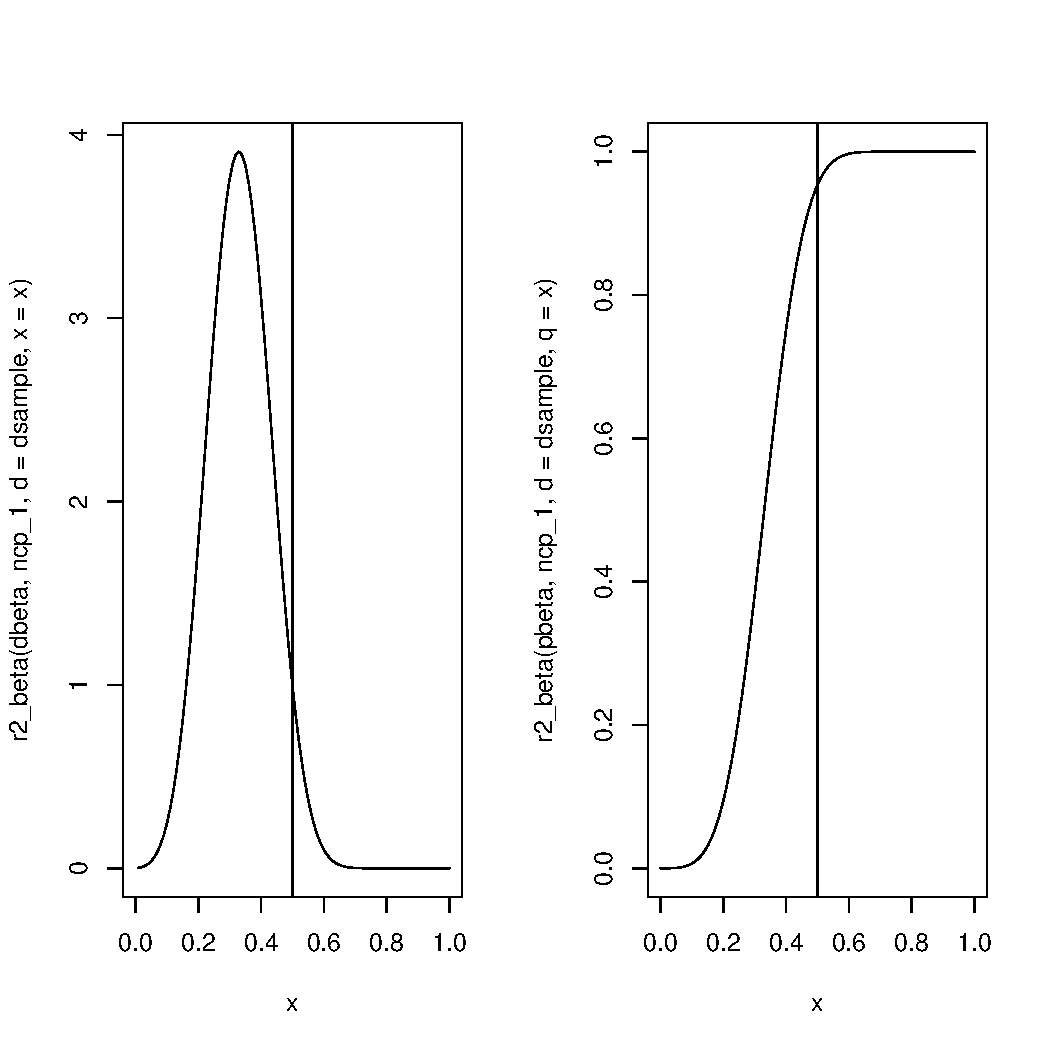
\includegraphics{2016_w09_files/figure-latex/unnamed-chunk-3-1.pdf}

Är detta enligt förväntan? Ser ut som att vi underskattar \(r^2\)
väldigt grovt \ldots{}?

\section{2016-03-01}\label{section-1}

Fortsätter titta på simuleringarna ovan. Gör om några ggr och finner att
det nog bara var slump att det blve så biased. Beöhver simulera flera
ggr men lite osäker på hur. Det bli rju olika fördelningar varje gång.
Ska jag beräkna medelvärden för \texttt{npc} eller på ngt sätt för hela
fördelningen?

\begin{Shaded}
\begin{Highlighting}[]
\KeywordTok{par}\NormalTok{(}\DataTypeTok{mfrow =} \KeywordTok{c}\NormalTok{(}\DecValTok{1}\NormalTok{,}\DecValTok{1}\NormalTok{))}
\KeywordTok{curve}\NormalTok{(}\KeywordTok{r2_beta}\NormalTok{(dbeta, ncp_1, }\DataTypeTok{d =} \NormalTok{dplyr::}\KeywordTok{sample_n}\NormalTok{(d, }\DecValTok{30}\NormalTok{), }\DataTypeTok{x =} \NormalTok{x)); }\KeywordTok{abline}\NormalTok{(}\DataTypeTok{v =} \NormalTok{.}\DecValTok{5}\NormalTok{)}
\KeywordTok{curve}\NormalTok{(}\KeywordTok{r2_beta}\NormalTok{(dbeta, ncp_1, }\DataTypeTok{d =} \NormalTok{dplyr::}\KeywordTok{sample_n}\NormalTok{(d, }\DecValTok{30}\NormalTok{), }\DataTypeTok{x =} \NormalTok{x), }\DataTypeTok{add =} \OtherTok{TRUE}\NormalTok{)}
\KeywordTok{curve}\NormalTok{(}\KeywordTok{r2_beta}\NormalTok{(dbeta, ncp_1, }\DataTypeTok{d =} \NormalTok{dplyr::}\KeywordTok{sample_n}\NormalTok{(d, }\DecValTok{30}\NormalTok{), }\DataTypeTok{x =} \NormalTok{x), }\DataTypeTok{add =} \OtherTok{TRUE}\NormalTok{)}
\KeywordTok{curve}\NormalTok{(}\KeywordTok{r2_beta}\NormalTok{(dbeta, ncp_1, }\DataTypeTok{d =} \NormalTok{dplyr::}\KeywordTok{sample_n}\NormalTok{(d, }\DecValTok{30}\NormalTok{), }\DataTypeTok{x =} \NormalTok{x), }\DataTypeTok{add =} \OtherTok{TRUE}\NormalTok{)}
\KeywordTok{curve}\NormalTok{(}\KeywordTok{r2_beta}\NormalTok{(dbeta, ncp_1, }\DataTypeTok{d =} \NormalTok{dplyr::}\KeywordTok{sample_n}\NormalTok{(d, }\DecValTok{30}\NormalTok{), }\DataTypeTok{x =} \NormalTok{x), }\DataTypeTok{add =} \OtherTok{TRUE}\NormalTok{)}
\KeywordTok{curve}\NormalTok{(}\KeywordTok{r2_beta}\NormalTok{(dbeta, ncp_1, }\DataTypeTok{d =} \NormalTok{dplyr::}\KeywordTok{sample_n}\NormalTok{(d, }\DecValTok{30}\NormalTok{), }\DataTypeTok{x =} \NormalTok{x), }\DataTypeTok{add =} \OtherTok{TRUE}\NormalTok{)}
\KeywordTok{curve}\NormalTok{(}\KeywordTok{r2_beta}\NormalTok{(dbeta, ncp_1, }\DataTypeTok{d =} \NormalTok{dplyr::}\KeywordTok{sample_n}\NormalTok{(d, }\DecValTok{30}\NormalTok{), }\DataTypeTok{x =} \NormalTok{x), }\DataTypeTok{add =} \OtherTok{TRUE}\NormalTok{)}
\KeywordTok{curve}\NormalTok{(}\KeywordTok{r2_beta}\NormalTok{(dbeta, ncp_1, }\DataTypeTok{d =} \NormalTok{dplyr::}\KeywordTok{sample_n}\NormalTok{(d, }\DecValTok{30}\NormalTok{), }\DataTypeTok{x =} \NormalTok{x), }\DataTypeTok{add =} \OtherTok{TRUE}\NormalTok{)}
\KeywordTok{curve}\NormalTok{(}\KeywordTok{r2_beta}\NormalTok{(dbeta, ncp_1, }\DataTypeTok{d =} \NormalTok{dplyr::}\KeywordTok{sample_n}\NormalTok{(d, }\DecValTok{30}\NormalTok{), }\DataTypeTok{x =} \NormalTok{x), }\DataTypeTok{add =} \OtherTok{TRUE}\NormalTok{)}
\KeywordTok{curve}\NormalTok{(}\KeywordTok{r2_beta}\NormalTok{(dbeta, ncp_1, }\DataTypeTok{d =} \NormalTok{dplyr::}\KeywordTok{sample_n}\NormalTok{(d, }\DecValTok{30}\NormalTok{), }\DataTypeTok{x =} \NormalTok{x), }\DataTypeTok{add =} \OtherTok{TRUE}\NormalTok{)}
\KeywordTok{curve}\NormalTok{(}\KeywordTok{r2_beta}\NormalTok{(dbeta, ncp_1, }\DataTypeTok{d =} \NormalTok{dplyr::}\KeywordTok{sample_n}\NormalTok{(d, }\DecValTok{30}\NormalTok{), }\DataTypeTok{x =} \NormalTok{x), }\DataTypeTok{add =} \OtherTok{TRUE}\NormalTok{)}
\KeywordTok{curve}\NormalTok{(}\KeywordTok{r2_beta}\NormalTok{(dbeta, ncp_1, }\DataTypeTok{d =} \NormalTok{dplyr::}\KeywordTok{sample_n}\NormalTok{(d, }\DecValTok{30}\NormalTok{), }\DataTypeTok{x =} \NormalTok{x), }\DataTypeTok{add =} \OtherTok{TRUE}\NormalTok{)}
\KeywordTok{curve}\NormalTok{(}\KeywordTok{r2_beta}\NormalTok{(dbeta, ncp_1, }\DataTypeTok{d =} \NormalTok{dplyr::}\KeywordTok{sample_n}\NormalTok{(d, }\DecValTok{30}\NormalTok{), }\DataTypeTok{x =} \NormalTok{x), }\DataTypeTok{add =} \OtherTok{TRUE}\NormalTok{)}
\KeywordTok{curve}\NormalTok{(}\KeywordTok{r2_beta}\NormalTok{(dbeta, ncp_1, }\DataTypeTok{d =} \NormalTok{dplyr::}\KeywordTok{sample_n}\NormalTok{(d, }\DecValTok{30}\NormalTok{), }\DataTypeTok{x =} \NormalTok{x), }\DataTypeTok{add =} \OtherTok{TRUE}\NormalTok{)}
\KeywordTok{curve}\NormalTok{(}\KeywordTok{r2_beta}\NormalTok{(dbeta, ncp_1, }\DataTypeTok{d =} \NormalTok{dplyr::}\KeywordTok{sample_n}\NormalTok{(d, }\DecValTok{30}\NormalTok{), }\DataTypeTok{x =} \NormalTok{x), }\DataTypeTok{add =} \OtherTok{TRUE}\NormalTok{)}
\KeywordTok{curve}\NormalTok{(}\KeywordTok{r2_beta}\NormalTok{(dbeta, ncp_1, }\DataTypeTok{d =} \NormalTok{dplyr::}\KeywordTok{sample_n}\NormalTok{(d, }\DecValTok{30}\NormalTok{), }\DataTypeTok{x =} \NormalTok{x), }\DataTypeTok{add =} \OtherTok{TRUE}\NormalTok{)}
\KeywordTok{curve}\NormalTok{(}\KeywordTok{r2_beta}\NormalTok{(dbeta, ncp_1, }\DataTypeTok{d =} \NormalTok{dplyr::}\KeywordTok{sample_n}\NormalTok{(d, }\DecValTok{30}\NormalTok{), }\DataTypeTok{x =} \NormalTok{x), }\DataTypeTok{add =} \OtherTok{TRUE}\NormalTok{)}
\KeywordTok{curve}\NormalTok{(}\KeywordTok{r2_beta}\NormalTok{(dbeta, ncp_1, }\DataTypeTok{d =} \NormalTok{dplyr::}\KeywordTok{sample_n}\NormalTok{(d, }\DecValTok{30}\NormalTok{), }\DataTypeTok{x =} \NormalTok{x), }\DataTypeTok{add =} \OtherTok{TRUE}\NormalTok{)}
\KeywordTok{curve}\NormalTok{(}\KeywordTok{r2_beta}\NormalTok{(dbeta, ncp_1, }\DataTypeTok{d =} \NormalTok{dplyr::}\KeywordTok{sample_n}\NormalTok{(d, }\DecValTok{30}\NormalTok{), }\DataTypeTok{x =} \NormalTok{x), }\DataTypeTok{add =} \OtherTok{TRUE}\NormalTok{)}
\KeywordTok{curve}\NormalTok{(}\KeywordTok{r2_beta}\NormalTok{(dbeta, ncp_1, }\DataTypeTok{d =} \NormalTok{dplyr::}\KeywordTok{sample_n}\NormalTok{(d, }\DecValTok{30}\NormalTok{), }\DataTypeTok{x =} \NormalTok{x), }\DataTypeTok{add =} \OtherTok{TRUE}\NormalTok{)}
\KeywordTok{curve}\NormalTok{(}\KeywordTok{r2_beta}\NormalTok{(dbeta, ncp_1, }\DataTypeTok{d =} \NormalTok{dplyr::}\KeywordTok{sample_n}\NormalTok{(d, }\DecValTok{30}\NormalTok{), }\DataTypeTok{x =} \NormalTok{x), }\DataTypeTok{add =} \OtherTok{TRUE}\NormalTok{)}
\end{Highlighting}
\end{Shaded}

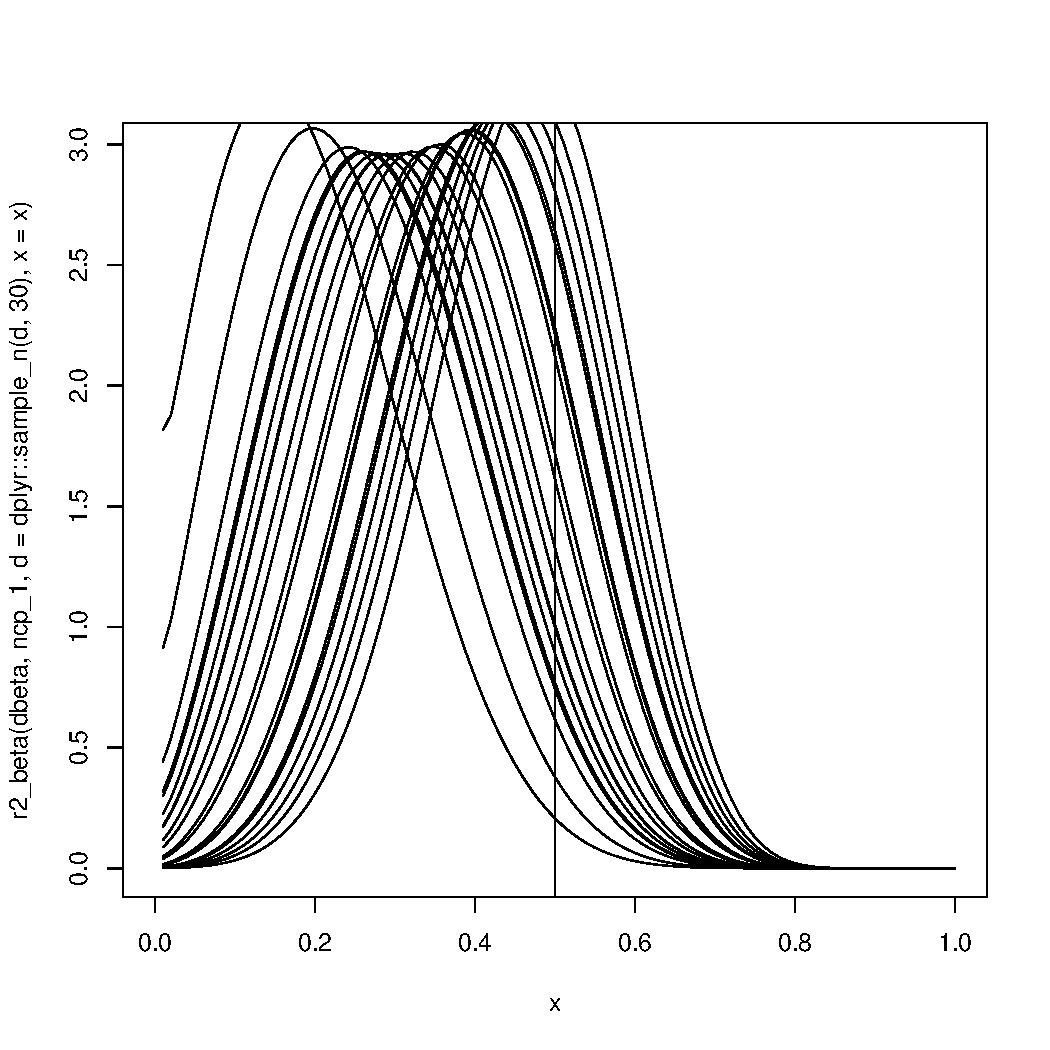
\includegraphics{2016_w09_files/figure-latex/unnamed-chunk-4-1.pdf}

\subsection{Diskussion med SN}\label{diskussion-med-sn}

Är ovanligt och lite konstigt att fördelningen i detta fall beror på
observerade data. För t ex t- och F-fördelning finns ju ett beroende av
frihetsgrad (stickprovsstorlek) men inte av själva datapunkterna. Att ha
ett sådant beroende känns lite märkligt då man på ngt sätt rättfärdigar
ett observerat resultat genom teorier byggda på samma observerade
resultat, vilket känns som ett cirkelresonameng. Å andra sidan är väl
just detta anledningen till att \(x\) enl teorin heller inte är att
betrakta som en slumpvariabel utan som fix.

Slutsatser:

\begin{enumerate}
\def\labelenumi{\arabic{enumi}.}
\tightlist
\item
  Det går inte att finna en enda teoretisk fördelning (facit) då den
  alltid kommer att bero på slumpen.
\item
  Vad vi kan göra är att koncentrera oss på t ex olika moment av
  fördelningen. Vi kan t ex ta ett stickprov och för detta beräkna både
  den semiteoretiska fördelning detta ger upphov till, samt skatta R2
  direkt. Vi jämför sedan skattningen mot värdet givet av väntevärdet
  givet av fördelningen. Vi upprepar många ggr och plottar dessa värden
  med qqplot för att undersöka ev bias.
\item
  Kan också vara av värde att undersöka ifall det finns metod att skatta
  betafördelningens parametrar utifrån data på ngt mer generellt sätt.
\end{enumerate}

Vi försöker göra enl (2) ovan. Dock behöver vi för detta jämföra
skattningen inte mot mean utan mot mode för att få det korrekt. Dock
svårt att finna ngn formel för mode av icke cenrtal betafördelning.
Finns funktion \texttt{modeest::betaMode} men den funktionen hanterar
ändå inte detta.

Enl (Park 1964) krävs numerisk approximation för skattning av mode för
icke-central beta. Formel presenteras i (3.2) men bygger på antaganden
(såsom att \(r^2 \rightarrow 1\)), vilket gör det hela ointeressant. Ett
alternativ blir då att skatta ett numeriskt värde (såsom vi också gjort
vid tidigare simulering), vilket vi lätt kan göra om vi antar att
fördelningen är unimodal, vilket vi här kan. Observera dock att vi här
inte ska basera mode-skattningen på vårt slumpmässiga urval utan på
fördelningens värde för \(\forall x: x \in [0,1]\) för relevant
fördelning. Kanske skulle man också kunna undersöka metoder för att
finna mode via paketet \texttt{modehunt}. Jag har ännu inte fördjupat
mig i det och vet således inte ifall det skulle ge annat resultat än min
egen mode-funktion.

\begin{Shaded}
\begin{Highlighting}[]
\NormalTok{r2_beta_mode <-}\StringTok{ }\NormalTok{function(ncp1, d, ...) \{}
  \NormalTok{x <-}\StringTok{ }\KeywordTok{seq}\NormalTok{(}\FloatTok{0.001}\NormalTok{, }\DecValTok{1}\NormalTok{, .}\DecValTok{001}\NormalTok{)}
  \NormalTok{y <-}\StringTok{ }\KeywordTok{r2_beta}\NormalTok{(dbeta, }\DataTypeTok{ncp1 =} \NormalTok{ncp1, }\DataTypeTok{d =} \NormalTok{d, }\DataTypeTok{x =} \NormalTok{x, ...)}
  \NormalTok{x[y ==}\StringTok{ }\KeywordTok{max}\NormalTok{(y)]}
\NormalTok{\}}

\CommentTok{# Prepare data sets}
\NormalTok{d <-}\StringTok{ }\KeywordTok{sim_data}\NormalTok{(}\DataTypeTok{r2 =} \NormalTok{.}\DecValTok{5}\NormalTok{, }\DataTypeTok{p =} \DecValTok{1}\NormalTok{)}
\NormalTok{ss <-}\StringTok{ }\KeywordTok{subsamples}\NormalTok{(d, }\DataTypeTok{n.max =} \DecValTok{30}\NormalTok{, }\DataTypeTok{N =} \DecValTok{1000}\NormalTok{)}
\NormalTok{ncp_1 <-}\StringTok{ }\KeywordTok{ncp1}\NormalTok{(d)}

\CommentTok{# Calculate "theoretical modes" and "observed r2"}
\NormalTok{modes <-}\StringTok{ }\KeywordTok{vapply}\NormalTok{(ss, function(d) }\KeywordTok{r2_beta_mode}\NormalTok{(ncp_1, d), }\KeywordTok{numeric}\NormalTok{(}\DecValTok{1}\NormalTok{))}
\NormalTok{r2s <-}\StringTok{ }\KeywordTok{metrics}\NormalTok{(ss, }\DataTypeTok{n.sample =} \DecValTok{30}\NormalTok{)$Rsquared}

\CommentTok{# Plot and compare}
\KeywordTok{par}\NormalTok{(}\DataTypeTok{mfrow =} \KeywordTok{c}\NormalTok{(}\DecValTok{1}\NormalTok{, }\DecValTok{2}\NormalTok{))}
\KeywordTok{plot}\NormalTok{(r2s, modes, }\DataTypeTok{xlim =} \KeywordTok{c}\NormalTok{(}\DecValTok{0}\NormalTok{, .}\DecValTok{8}\NormalTok{), }\DataTypeTok{ylim =} \KeywordTok{c}\NormalTok{(}\DecValTok{0}\NormalTok{, .}\DecValTok{6}\NormalTok{))}
\KeywordTok{abline}\NormalTok{(}\DecValTok{0}\NormalTok{, }\DecValTok{1}\NormalTok{)}
\KeywordTok{qqplot}\NormalTok{(r2s, modes)}
\end{Highlighting}
\end{Shaded}

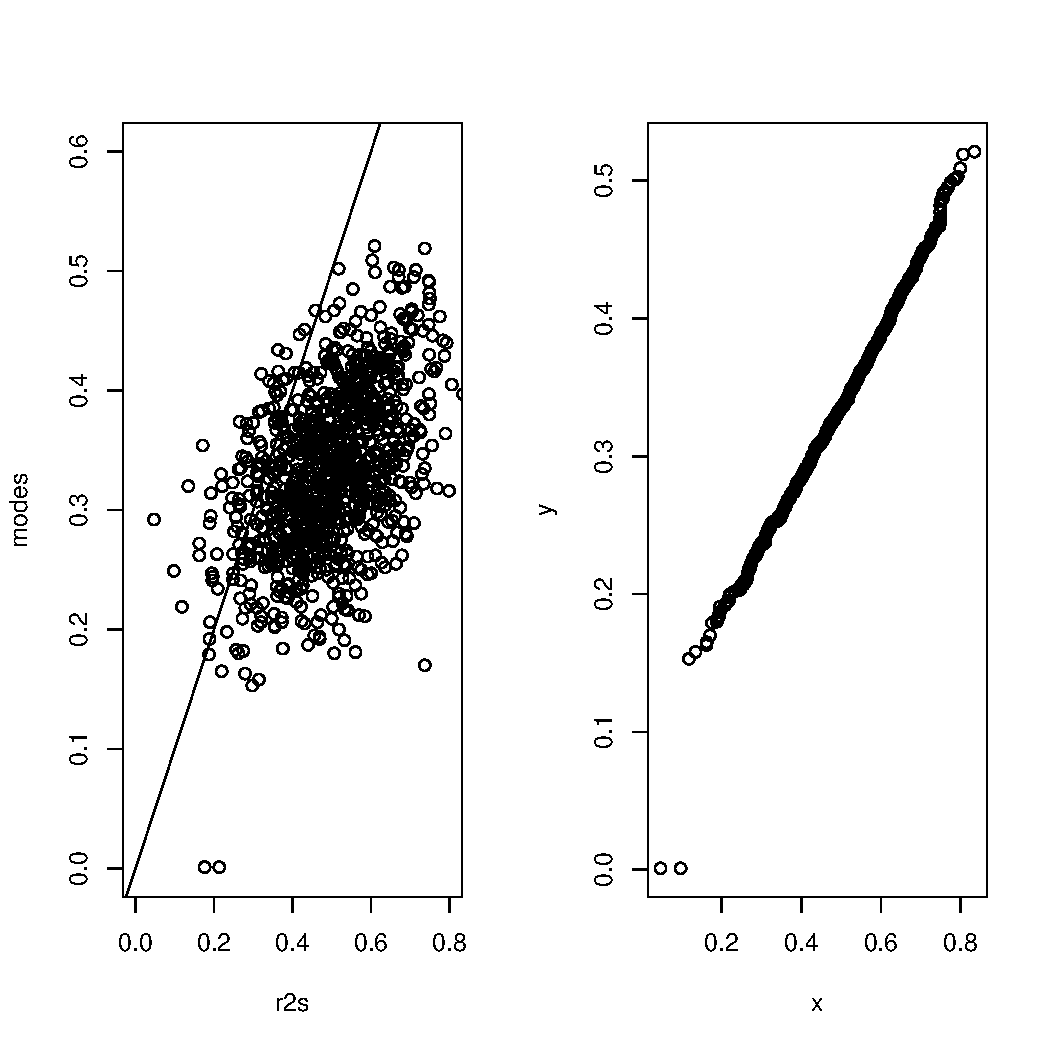
\includegraphics{2016_w09_files/figure-latex/unnamed-chunk-5-1.pdf} Vi
ser här att vår teoretiska mode underskattr vårt observerade värde. Är
det trots allt så att vi inte bör jämföra mot mode utan mot mean? Det
finns visserilgen en teoretisk formel för att beräkna mean av icke
cenrtal betafördelning men den behöver i sin tur en confluent
hypergeometric function. Det finns dock fler versioner av detta och de
som finns implementerade i R tycks inte motsvara den här aktuella. Vi
får därför skatta mean pss som vi tidigare skattade mode. Å andra sidan
har vi också en formel för väntevärdet av \(r^2\) för selektive samlpnig
given av (Warren 1971) avs 2.2. Även här refereras till en confluent
hypergeometric function men då denna har endast tre variabler är
sannolikheten större att denna är samma som t ex
\texttt{hypergeo::genhypergeo}. Dock krävs fler parametrar som jag inble
blir riktigt klok på (tycks smo att man ska slumpa \(n\) värden från
varje punkt tagen med selective samplnig men jag får inte riktigt ihop
det).

\begin{Shaded}
\begin{Highlighting}[]
\NormalTok{r2_beta_mean <-}\StringTok{ }\NormalTok{function(ncp1, d, ...) \{}
  \NormalTok{x <-}\StringTok{ }\KeywordTok{seq}\NormalTok{(}\FloatTok{0.001}\NormalTok{, }\DecValTok{1}\NormalTok{, .}\DecValTok{001}\NormalTok{)}
  \NormalTok{y <-}\StringTok{ }\KeywordTok{r2_beta}\NormalTok{(dbeta, }\DataTypeTok{ncp1 =} \NormalTok{ncp1, }\DataTypeTok{d =} \NormalTok{d, }\DataTypeTok{x =} \NormalTok{x, ...)}
  \KeywordTok{sum}\NormalTok{((y /}\StringTok{ }\KeywordTok{sum}\NormalTok{(y)) *}\StringTok{ }\NormalTok{x)}
\NormalTok{\}}

\CommentTok{# Calculate "theoretical modes" and "observed r2"}
\NormalTok{means <-}\StringTok{ }\KeywordTok{vapply}\NormalTok{(ss, function(d) }\KeywordTok{r2_beta_mean}\NormalTok{(ncp_1, d), }\KeywordTok{numeric}\NormalTok{(}\DecValTok{1}\NormalTok{))}

\CommentTok{# Plot and compare}
\KeywordTok{par}\NormalTok{(}\DataTypeTok{mfrow =} \KeywordTok{c}\NormalTok{(}\DecValTok{2}\NormalTok{, }\DecValTok{2}\NormalTok{))}
\KeywordTok{plot}\NormalTok{(r2s, means, }\DataTypeTok{xlim =} \KeywordTok{c}\NormalTok{(}\DecValTok{0}\NormalTok{, .}\DecValTok{8}\NormalTok{), }\DataTypeTok{ylim =} \KeywordTok{c}\NormalTok{(}\DecValTok{0}\NormalTok{, .}\DecValTok{8}\NormalTok{), }\DataTypeTok{main =} \StringTok{"Comparison to mean"}\NormalTok{)}
  \KeywordTok{abline}\NormalTok{(}\DecValTok{0}\NormalTok{, }\DecValTok{1}\NormalTok{); }\KeywordTok{points}\NormalTok{(.}\DecValTok{5}\NormalTok{, .}\DecValTok{5}\NormalTok{, }\DataTypeTok{lwd =} \DecValTok{5}\NormalTok{, }\DataTypeTok{col =} \StringTok{"red"}\NormalTok{)}
\KeywordTok{qqplot}\NormalTok{(r2s, means, }\DataTypeTok{xlim =} \KeywordTok{c}\NormalTok{(}\DecValTok{0}\NormalTok{, .}\DecValTok{8}\NormalTok{), }\DataTypeTok{ylim =} \KeywordTok{c}\NormalTok{(}\DecValTok{0}\NormalTok{, .}\DecValTok{8}\NormalTok{), }\DataTypeTok{main =} \StringTok{"Comparison to mean"}\NormalTok{)}
  \KeywordTok{abline}\NormalTok{(}\DecValTok{0}\NormalTok{, }\DecValTok{1}\NormalTok{) }
\KeywordTok{plot}\NormalTok{(r2s, modes, }\DataTypeTok{xlim =} \KeywordTok{c}\NormalTok{(}\DecValTok{0}\NormalTok{, .}\DecValTok{8}\NormalTok{), }\DataTypeTok{ylim =} \KeywordTok{c}\NormalTok{(}\DecValTok{0}\NormalTok{, .}\DecValTok{8}\NormalTok{), }\DataTypeTok{main =} \StringTok{"Comparison to mdoe"}\NormalTok{)}
  \KeywordTok{abline}\NormalTok{(}\DecValTok{0}\NormalTok{, }\DecValTok{1}\NormalTok{); }\KeywordTok{points}\NormalTok{(.}\DecValTok{5}\NormalTok{, .}\DecValTok{5}\NormalTok{, }\DataTypeTok{lwd =} \DecValTok{5}\NormalTok{, }\DataTypeTok{col =} \StringTok{"red"}\NormalTok{)}
\KeywordTok{qqplot}\NormalTok{(r2s, modes, }\DataTypeTok{xlim =} \KeywordTok{c}\NormalTok{(}\DecValTok{0}\NormalTok{, .}\DecValTok{8}\NormalTok{), }\DataTypeTok{ylim =} \KeywordTok{c}\NormalTok{(}\DecValTok{0}\NormalTok{, .}\DecValTok{8}\NormalTok{), }\DataTypeTok{main =} \StringTok{"Comparison to mode"}\NormalTok{)}
  \KeywordTok{abline}\NormalTok{(}\DecValTok{0}\NormalTok{, }\DecValTok{1}\NormalTok{) }
\end{Highlighting}
\end{Shaded}

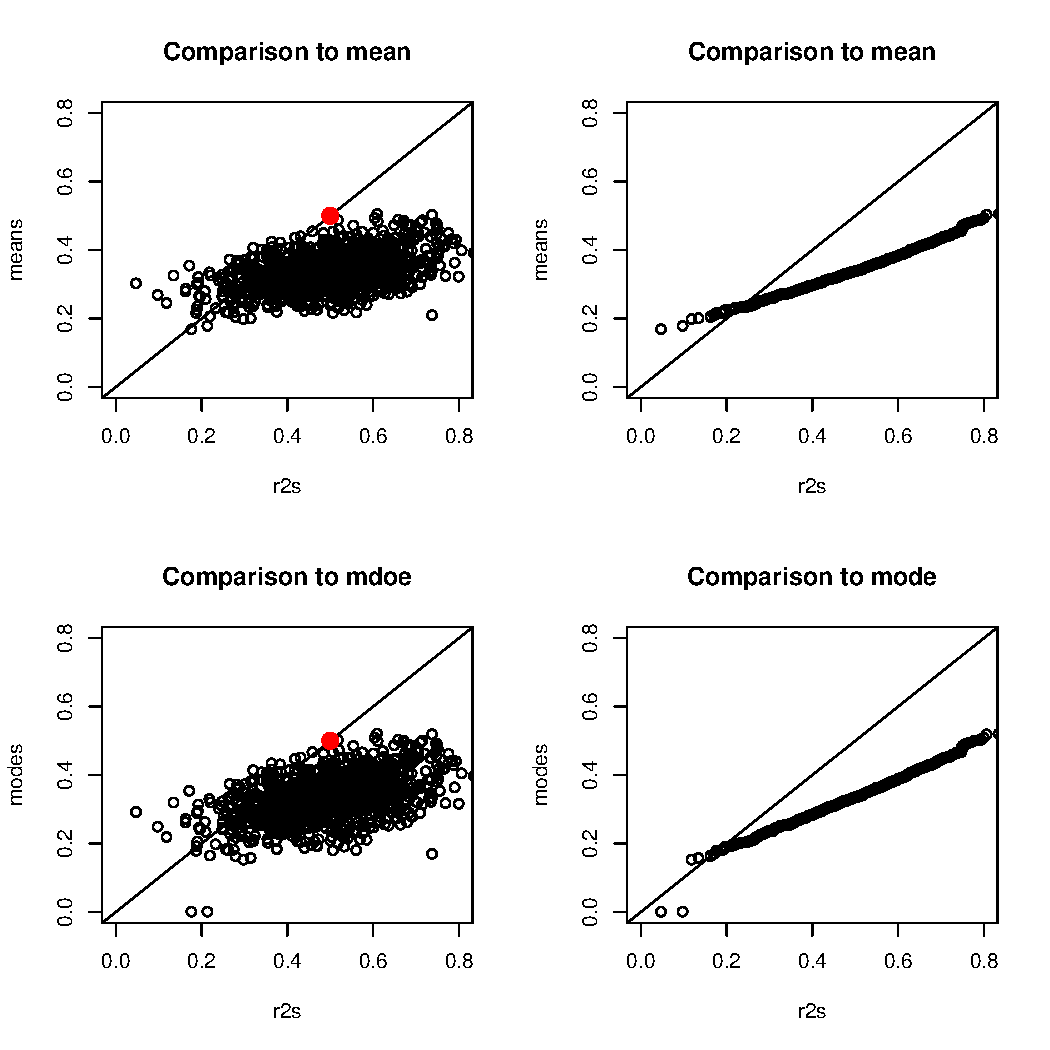
\includegraphics{2016_w09_files/figure-latex/unnamed-chunk-6-1.pdf}

Röda prickar markerar \(\rho^2\) men observera här att värden på y-axeln
(mean resp mode) inte syftar till att approximera det teoretiska värdet
utan värdet för \(r^2\), vilket vi vet underskattar \(\rho^2\) för varje
enskild observation. Om \(r^2\) skulle följa den ickecenrtala
betafördelningen skulle vi dock se observationer centrerade kring linjen
i graferna. Det gör vi inte. Vad vi ser är istället att den teoretiska
fördelningen tycks underskatta observerade \(r^2\) systematiskt. Vi ser
endast marginell skillnad mellan mode och mean (tyder väl på att den
teoretiska fördelningen är mindre skev än den verkliga?) men möjligt att
mode är lite bättre (vilket stämmer med teorin).

\textbf{Slutsats:} Den icke centrala betafördelningen enligt (Hogben
1968) underskattar \(r^2\).

Men för att sammanfatta så avviker jag också från teorin enl:

\begin{enumerate}
\def\labelenumi{\arabic{enumi}.}
\tightlist
\item
  Mitt x slumpas (ej fixt). Vet dock inte riktigt hur detta bör påverka
  resultatet.
\item
  Mode och mean från fördelningen är skattade på kanske inte allra bästa
  sätt? Ett alternativ är kanske att nyttja fördelningen till att slumpa
  fram en massa värden och sedan beräkna mode och mean av det. Tycker
  dock inte det borde bli ngn skillnad \ldots{} men kan ju förstås testa
  \ldots{}
\end{enumerate}

\begin{Shaded}
\begin{Highlighting}[]
\NormalTok{mode <-}\StringTok{ }\NormalTok{function(d) \{}
  \NormalTok{z <-}\StringTok{ }\KeywordTok{density}\NormalTok{(d)}
  \NormalTok{z$x[z$y ==}\StringTok{ }\KeywordTok{max}\NormalTok{(z$y)]}
\NormalTok{\}}

\CommentTok{# Mode baserat på simulering}
\NormalTok{r2_beta_mode_r <-}\StringTok{ }\NormalTok{function(ncp1, d, ...) \{}
  \NormalTok{y <-}\StringTok{ }\KeywordTok{r2_beta}\NormalTok{(rbeta, }\DataTypeTok{ncp1 =} \NormalTok{ncp1, }\DataTypeTok{d =} \NormalTok{d, }\DataTypeTok{n =} \FloatTok{1e4}\NormalTok{, ...)}
  \KeywordTok{mode}\NormalTok{(y)}
\NormalTok{\}}
\NormalTok{modesr <-}\StringTok{ }\KeywordTok{vapply}\NormalTok{(ss, function(d) }\KeywordTok{r2_beta_mode_r}\NormalTok{(ncp_1, d), }\KeywordTok{numeric}\NormalTok{(}\DecValTok{1}\NormalTok{))}

\CommentTok{# Kollar om det finns ngn skillnad mellan de två sätten }
\KeywordTok{t.test}\NormalTok{(modes, modesr)}
\end{Highlighting}
\end{Shaded}

\begin{verbatim}
## 
##  Welch Two Sample t-test
## 
## data:  modes and modesr
## t = 0.010579, df = 1997.9, p-value = 0.9916
## alternative hypothesis: true difference in means is not equal to 0
## 95 percent confidence interval:
##  -0.005944838  0.006009319
## sample estimates:
## mean of x mean of y 
## 0.3340960 0.3340638
\end{verbatim}

\begin{Shaded}
\begin{Highlighting}[]
\CommentTok{# Mean baserat på simulering}
\NormalTok{r2_beta_mean_r <-}\StringTok{ }\NormalTok{function(ncp1, d, ...) \{}
  \NormalTok{y <-}\StringTok{ }\KeywordTok{r2_beta}\NormalTok{(rbeta, }\DataTypeTok{ncp1 =} \NormalTok{ncp1, }\DataTypeTok{d =} \NormalTok{d, }\DataTypeTok{n =} \FloatTok{1e4}\NormalTok{, ...)}
  \KeywordTok{mean}\NormalTok{(y)}
\NormalTok{\}}
\NormalTok{meansr <-}\StringTok{ }\KeywordTok{vapply}\NormalTok{(ss, function(d) }\KeywordTok{r2_beta_mode_r}\NormalTok{(ncp_1, d), }\KeywordTok{numeric}\NormalTok{(}\DecValTok{1}\NormalTok{))}

\CommentTok{# Kollar om det finns ngn skillnad mellan de två sätten }
\KeywordTok{t.test}\NormalTok{(means, meansr)}
\end{Highlighting}
\end{Shaded}

\begin{verbatim}
## 
##  Welch Two Sample t-test
## 
## data:  means and meansr
## t = 1.3111, df = 1923.7, p-value = 0.19
## alternative hypothesis: true difference in means is not equal to 0
## 95 percent confidence interval:
##  -0.001819645  0.009159424
## sample estimates:
## mean of x mean of y 
## 0.3393171 0.3356472
\end{verbatim}

Alltså ingen skillnad för mode. Skillanden för mean är större men
fortfarande inte signifikant.

\begin{Shaded}
\begin{Highlighting}[]
\KeywordTok{par}\NormalTok{(}\DataTypeTok{mfrow =} \KeywordTok{c}\NormalTok{(}\DecValTok{1}\NormalTok{, }\DecValTok{2}\NormalTok{))}
\KeywordTok{plot}\NormalTok{(r2s, meansr, }\DataTypeTok{xlim =} \KeywordTok{c}\NormalTok{(}\DecValTok{0}\NormalTok{, .}\DecValTok{8}\NormalTok{), }\DataTypeTok{ylim =} \KeywordTok{c}\NormalTok{(}\DecValTok{0}\NormalTok{, .}\DecValTok{8}\NormalTok{), }\DataTypeTok{main =} \StringTok{"Comparison to mean"}\NormalTok{)}
  \KeywordTok{abline}\NormalTok{(}\DecValTok{0}\NormalTok{, }\DecValTok{1}\NormalTok{); }\KeywordTok{points}\NormalTok{(.}\DecValTok{5}\NormalTok{, .}\DecValTok{5}\NormalTok{, }\DataTypeTok{lwd =} \DecValTok{5}\NormalTok{, }\DataTypeTok{col =} \StringTok{"red"}\NormalTok{)}
\KeywordTok{qqplot}\NormalTok{(r2s, meansr, }\DataTypeTok{xlim =} \KeywordTok{c}\NormalTok{(}\DecValTok{0}\NormalTok{, .}\DecValTok{8}\NormalTok{), }\DataTypeTok{ylim =} \KeywordTok{c}\NormalTok{(}\DecValTok{0}\NormalTok{, .}\DecValTok{8}\NormalTok{), }\DataTypeTok{main =} \StringTok{"Comparison to mean"}\NormalTok{)}
  \KeywordTok{abline}\NormalTok{(}\DecValTok{0}\NormalTok{, }\DecValTok{1}\NormalTok{) }
\end{Highlighting}
\end{Shaded}

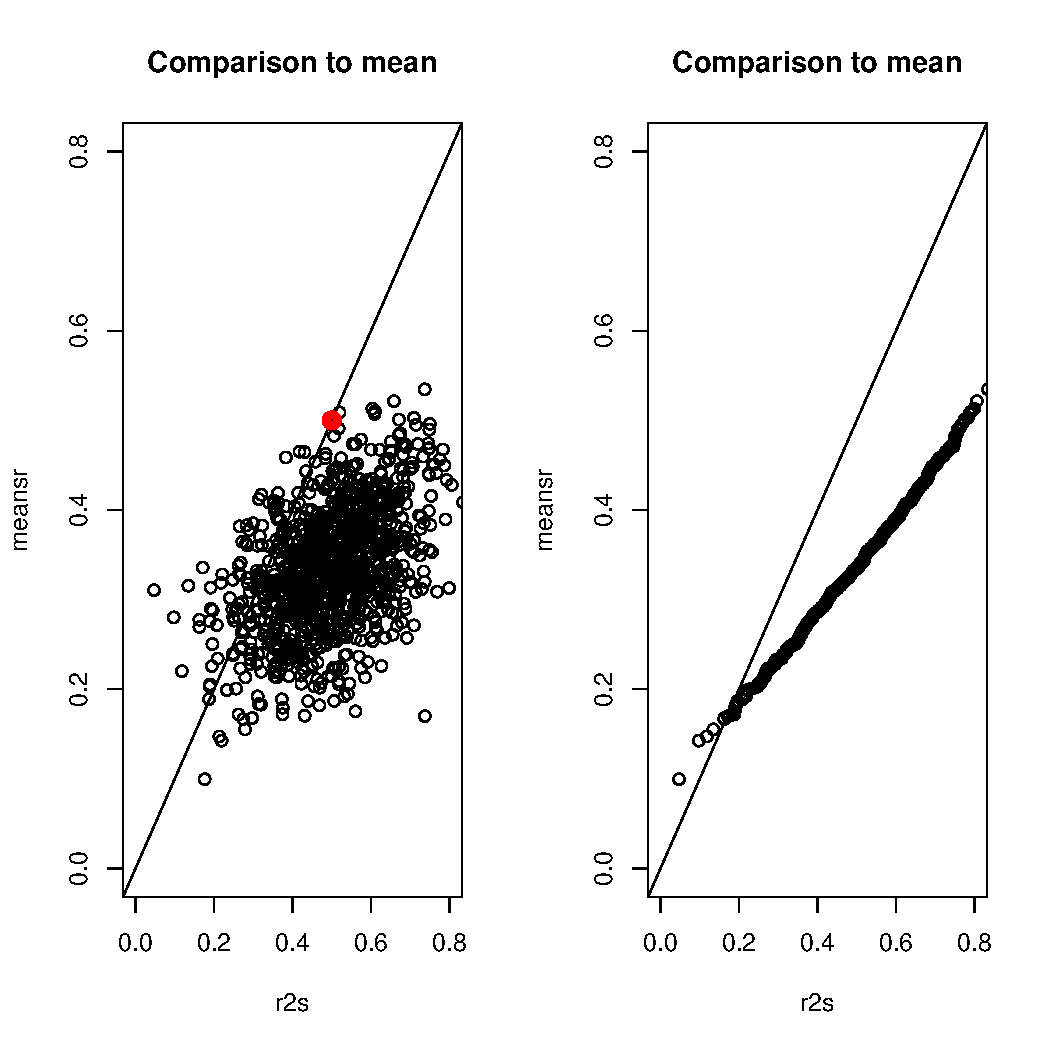
\includegraphics{2016_w09_files/figure-latex/unnamed-chunk-8-1.pdf}

Noterar f.ö. att endast (Warren 1971) (samt en artikel som tycks
irrelevant i sammanhanget) refererar till (Hogben 1968). Gissar därför
att man inte har nyttjat dessa resultat i ngn större utsträckning. Det
finns fler referenser till (Warren 1971). Jag har gått igenom dem och
lagt till i läslistan.

Hade kanske vart intressant att t ex också jämföra med normalfördelning
för att se vilken fördelning av dessa som är bäst och i så fall hur stor
skillnaden kan vara.

\subsection{Läsning av (Delignette-muller and Dutang
2015)}\label{lasning-av-fitdistrplus}

Utgår från ML-skattningar. Kan skatta både fördelning och dess
parametrar. Kan också baseras på ``maximum goodness-of-fit''.

\texttt{descdist}-funktionen medger också att beräkningar kan ta hänsyn
till bias eller inte. Tyvärr tycke det inte möjligt att inkludera
ickecentraliseringsparametern för skattning utan bara
shape-paramterarna. Har försökt studera koden i paketet men finnser där
ingen klar förklaring till varför. Kan det vara ngn skillnad som finns
inbyggd i själva betafunktionerna? Samtliga Beta-funktioner nyttjar
intern C-kod men jag kan se att man gör tydlig skillnad på just
\texttt{ncp}-parametern (dock baserat på om den är missing och inte 0,
vilket faktiskt är default \ldots{} förstår inte riktigt!?)

Går app skapa enskilda plottar av \texttt{fitdist}-objekt mha
\texttt{denscomp}, \texttt{cdfcomp}, \texttt{qqcomp}och \texttt{ppcomp}.

\begin{Shaded}
\begin{Highlighting}[]
\KeywordTok{library}\NormalTok{(}\StringTok{"fitdistrplus"}\NormalTok{)}
\NormalTok{ss <-}\StringTok{ }\KeywordTok{sim_data}\NormalTok{(}\DataTypeTok{r2 =} \NormalTok{.}\DecValTok{5}\NormalTok{, }\DataTypeTok{p =} \DecValTok{1}\NormalTok{) %>%}\StringTok{ }
\StringTok{  }\KeywordTok{subsamples}\NormalTok{(}\DataTypeTok{n.max =} \DecValTok{500}\NormalTok{, }\DataTypeTok{N =} \DecValTok{1000}\NormalTok{)}
\NormalTok{m <-}\StringTok{ }\KeywordTok{metrics}\NormalTok{(ss, }\DataTypeTok{n.sample =} \KeywordTok{c}\NormalTok{(}\DecValTok{10}\NormalTok{, }\DecValTok{20}\NormalTok{, }\DecValTok{30}\NormalTok{, }\DecValTok{50}\NormalTok{, }\DecValTok{100}\NormalTok{, }\DecValTok{200}\NormalTok{, }\DecValTok{300}\NormalTok{, }\DecValTok{400}\NormalTok{, }\DecValTok{500}\NormalTok{))}
\NormalTok{R2 <-}\StringTok{ }\KeywordTok{as.data.frame}\NormalTok{(m$Rsquared)}

\CommentTok{# Tycks här som att vi har en betafördelningt för n upp till ca 30}
\CommentTok{# Dock för n = 200 tycks vi kunna använda gammafördelning för approximation}
\CommentTok{# Från kanske n = 200 tycks normalapproximation kunna fungera bra. }
\KeywordTok{par}\NormalTok{(}\DataTypeTok{mfrow =} \KeywordTok{c}\NormalTok{(}\DecValTok{3}\NormalTok{, }\DecValTok{3}\NormalTok{)); }\KeywordTok{lapply}\NormalTok{(R2, descdist, }\DataTypeTok{boot =} \DecValTok{1000}\NormalTok{)}
\end{Highlighting}
\end{Shaded}

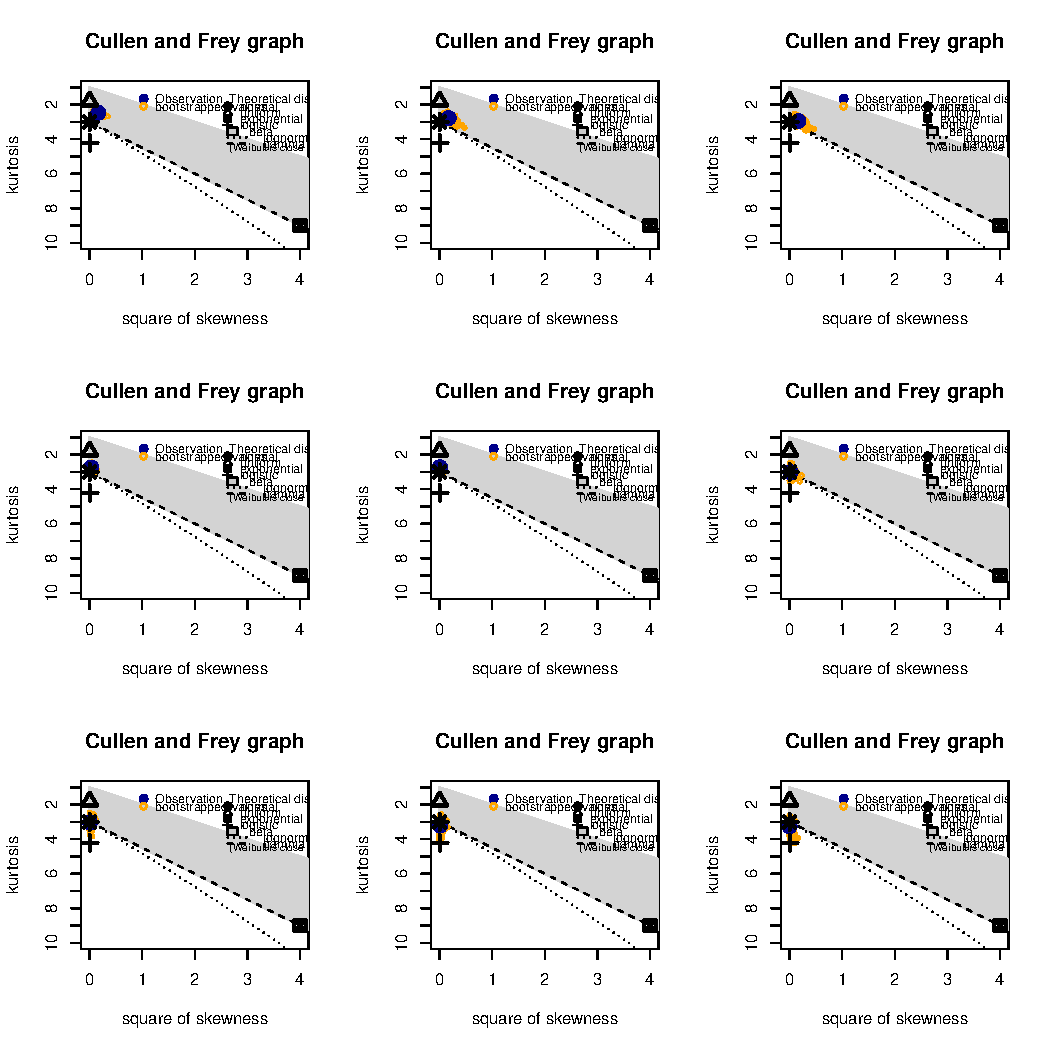
\includegraphics{2016_w09_files/figure-latex/unnamed-chunk-9-1.pdf}

\begin{Shaded}
\begin{Highlighting}[]
\CommentTok{# Jag gör en större plot för just n = 200 för att kolla lite närmare på just detta}
\CommentTok{# Ser här att en gammafördelning verkar kunna passa rätt bra.}
\KeywordTok{par}\NormalTok{(}\DataTypeTok{mfrow =} \KeywordTok{c}\NormalTok{(}\DecValTok{1}\NormalTok{, }\DecValTok{1}\NormalTok{)); }\KeywordTok{descdist}\NormalTok{(R2[, }\DecValTok{6}\NormalTok{], }\DataTypeTok{boot =} \DecValTok{10000}\NormalTok{)}
\end{Highlighting}
\end{Shaded}

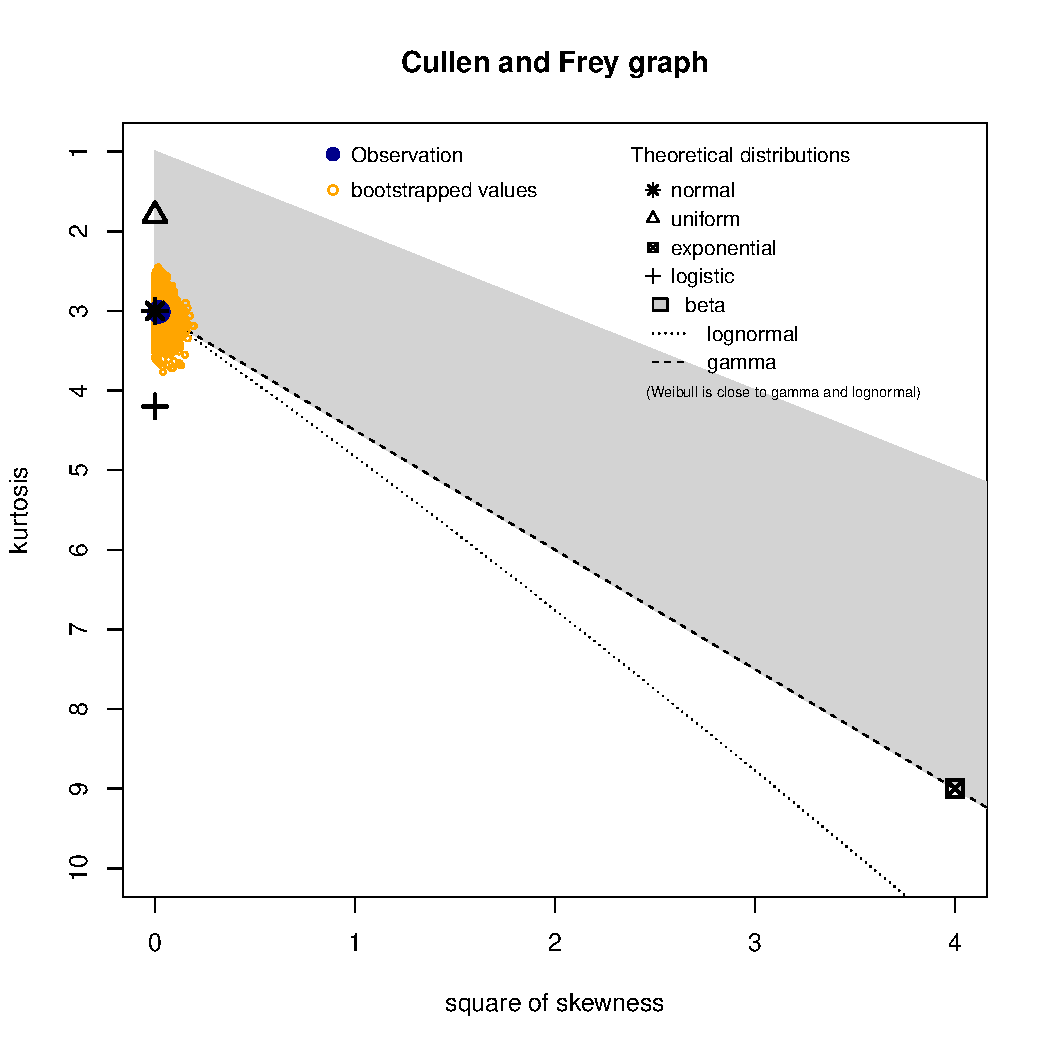
\includegraphics{2016_w09_files/figure-latex/unnamed-chunk-9-2.pdf}

\begin{Shaded}
\begin{Highlighting}[]
\CommentTok{# Ser här att en normalfördelning verkar kunna passa rätt bra vid n = 300}
\KeywordTok{par}\NormalTok{(}\DataTypeTok{mfrow =} \KeywordTok{c}\NormalTok{(}\DecValTok{1}\NormalTok{, }\DecValTok{1}\NormalTok{)); }\KeywordTok{descdist}\NormalTok{(R2[, }\DecValTok{7}\NormalTok{], }\DataTypeTok{boot =} \DecValTok{10000}\NormalTok{)}
\end{Highlighting}
\end{Shaded}

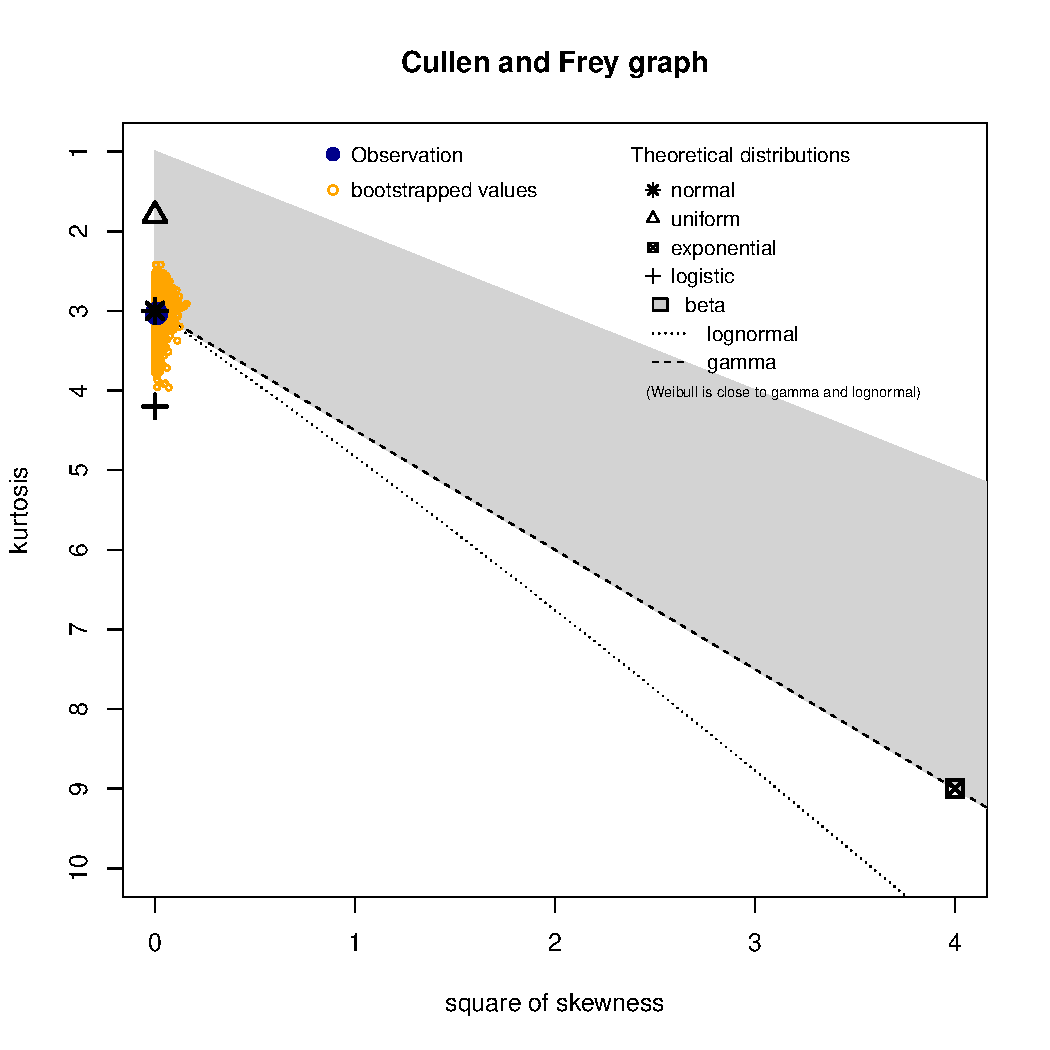
\includegraphics{2016_w09_files/figure-latex/unnamed-chunk-9-3.pdf}

\begin{Shaded}
\begin{Highlighting}[]
\CommentTok{# Vill testa att anpassa en betafördelning}
\CommentTok{# Tydligen estimeras bara shape1 och shape2, inte ncp (vilket gör att resultatet inte blir jättebra)}

\KeywordTok{lapply}\NormalTok{(R2, function(x) \{}
  \NormalTok{fit <-}\StringTok{ }\KeywordTok{fitdist}\NormalTok{(x, }\StringTok{"beta"}\NormalTok{)}
  \KeywordTok{plotdist}\NormalTok{(x, }\StringTok{"beta"}\NormalTok{, }\DataTypeTok{para =} \KeywordTok{list}\NormalTok{(}\DataTypeTok{shape1 =} \NormalTok{fit$estimate[}\DecValTok{1}\NormalTok{], }\DataTypeTok{shape2 =} \NormalTok{fit$estimate[}\DecValTok{2}\NormalTok{]))}
\NormalTok{\})}
\end{Highlighting}
\end{Shaded}

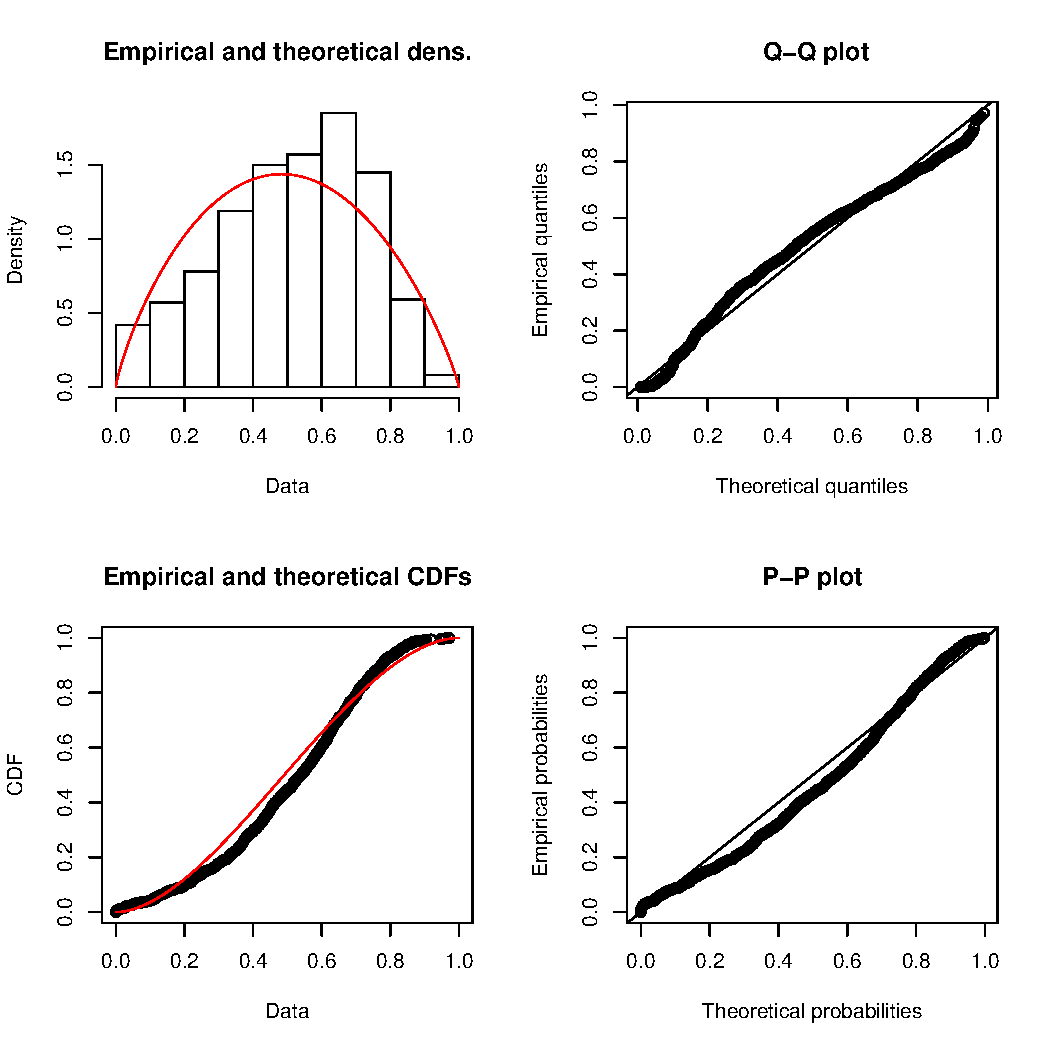
\includegraphics{2016_w09_files/figure-latex/unnamed-chunk-9-4.pdf}
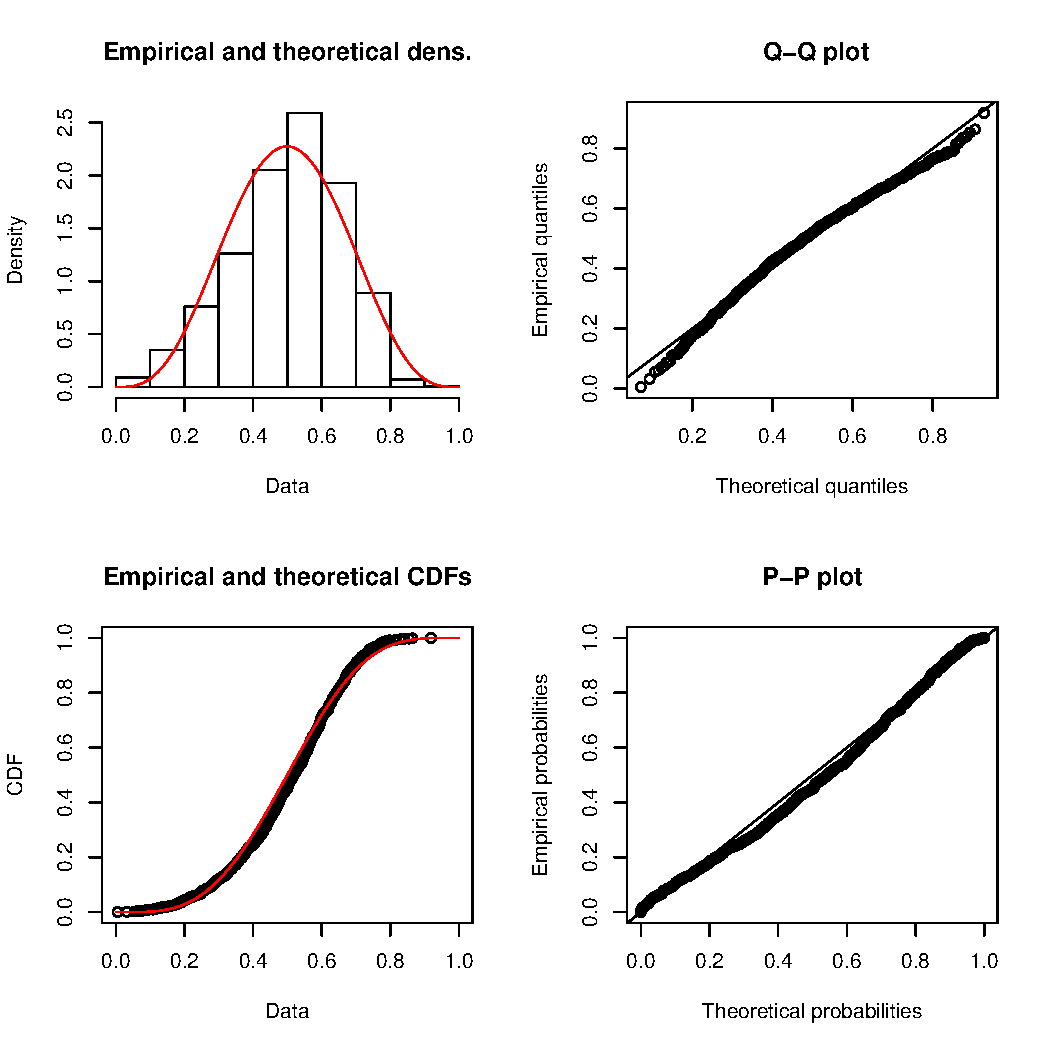
\includegraphics{2016_w09_files/figure-latex/unnamed-chunk-9-5.pdf}
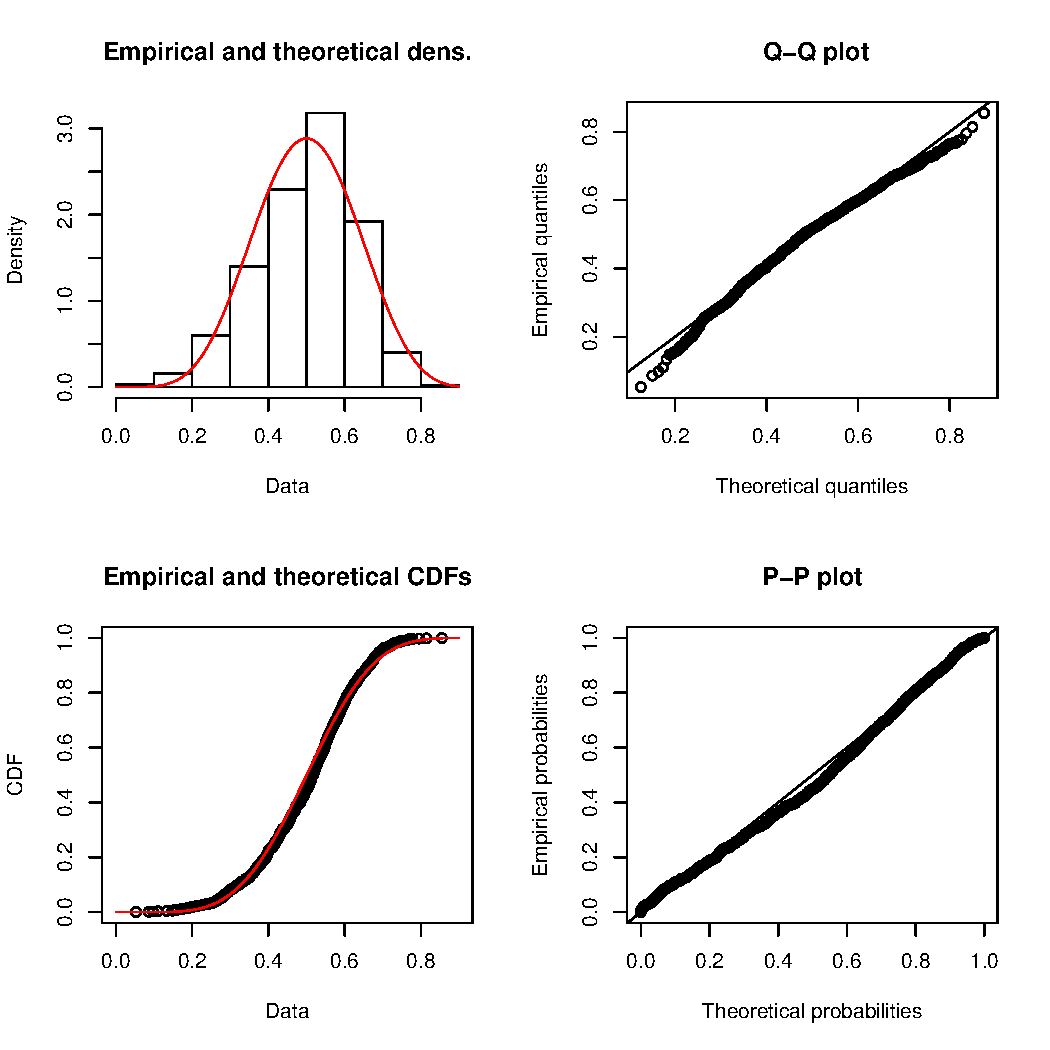
\includegraphics{2016_w09_files/figure-latex/unnamed-chunk-9-6.pdf}
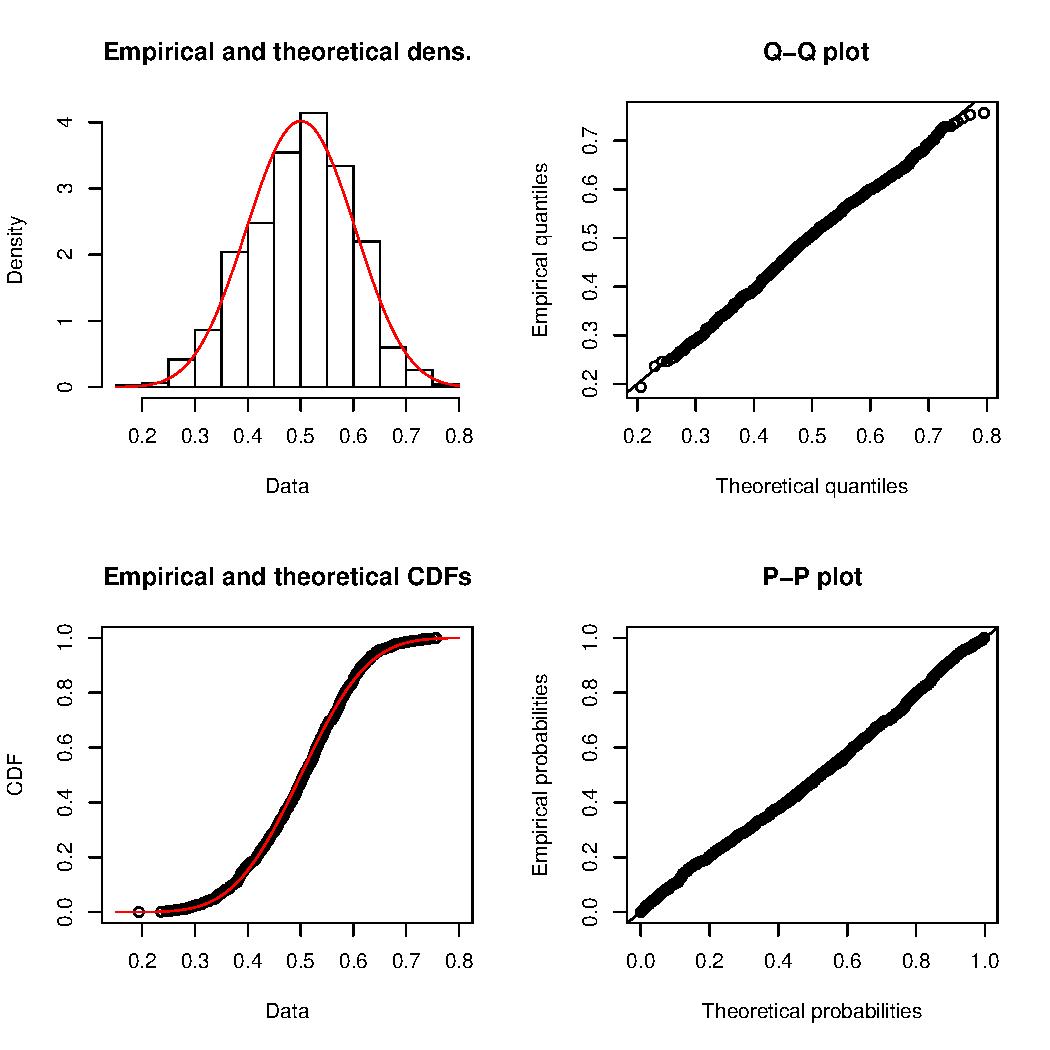
\includegraphics{2016_w09_files/figure-latex/unnamed-chunk-9-7.pdf}
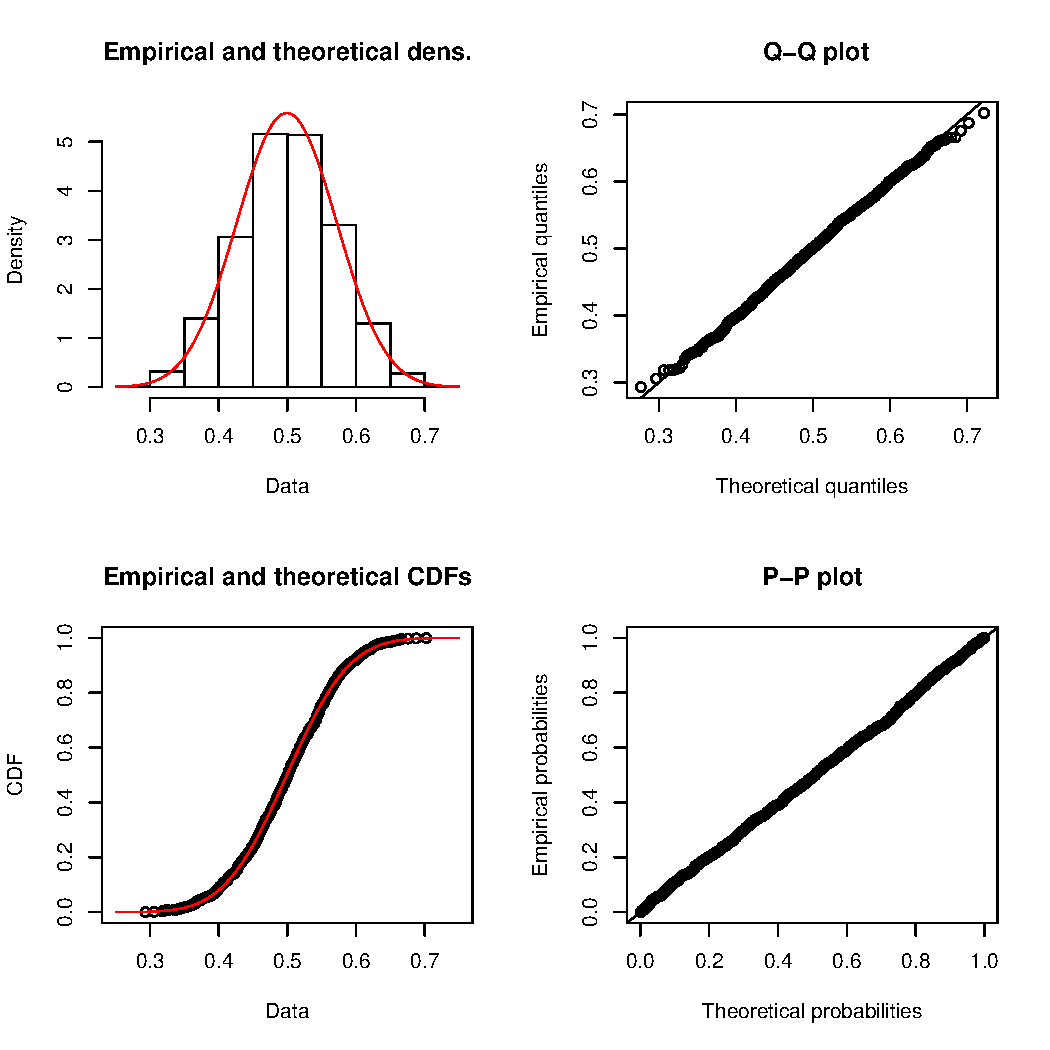
\includegraphics{2016_w09_files/figure-latex/unnamed-chunk-9-8.pdf}
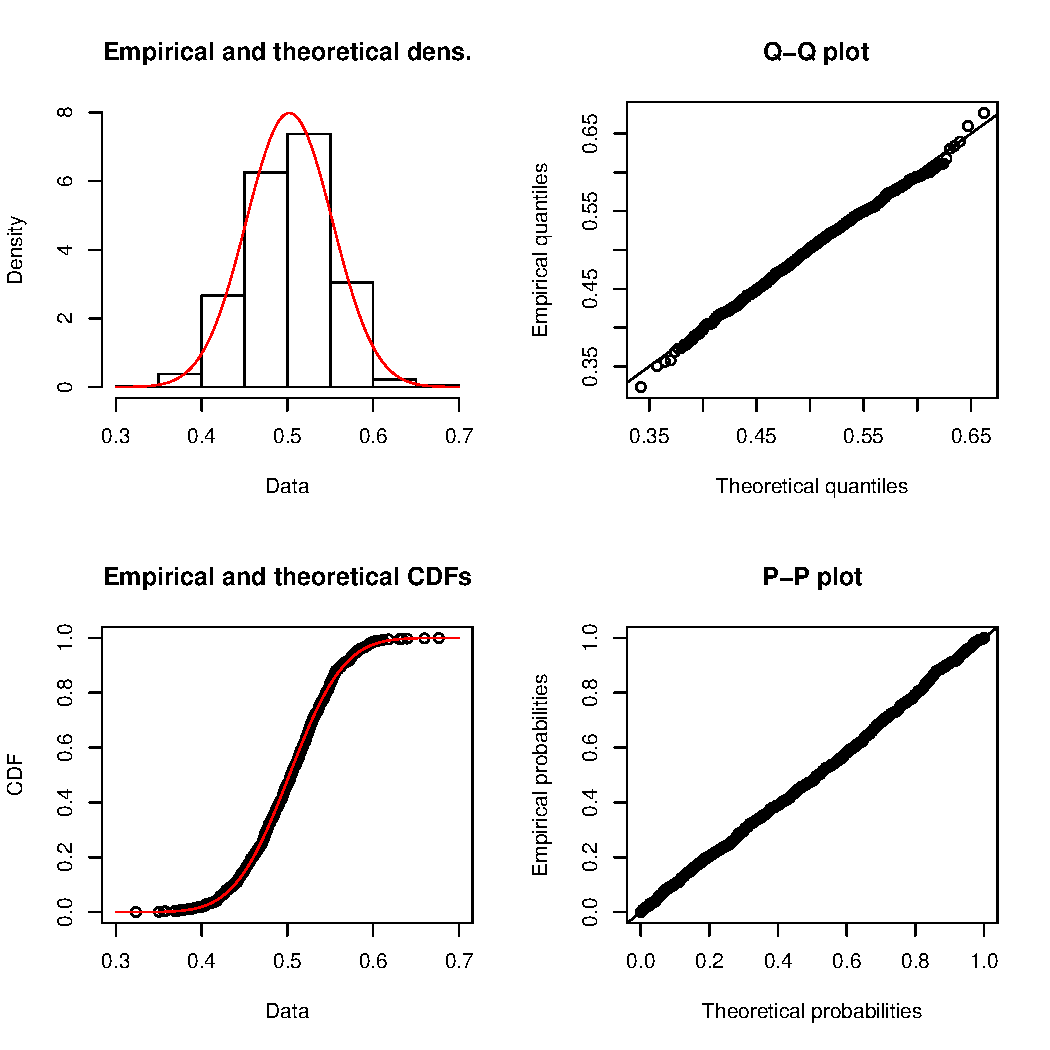
\includegraphics{2016_w09_files/figure-latex/unnamed-chunk-9-9.pdf}
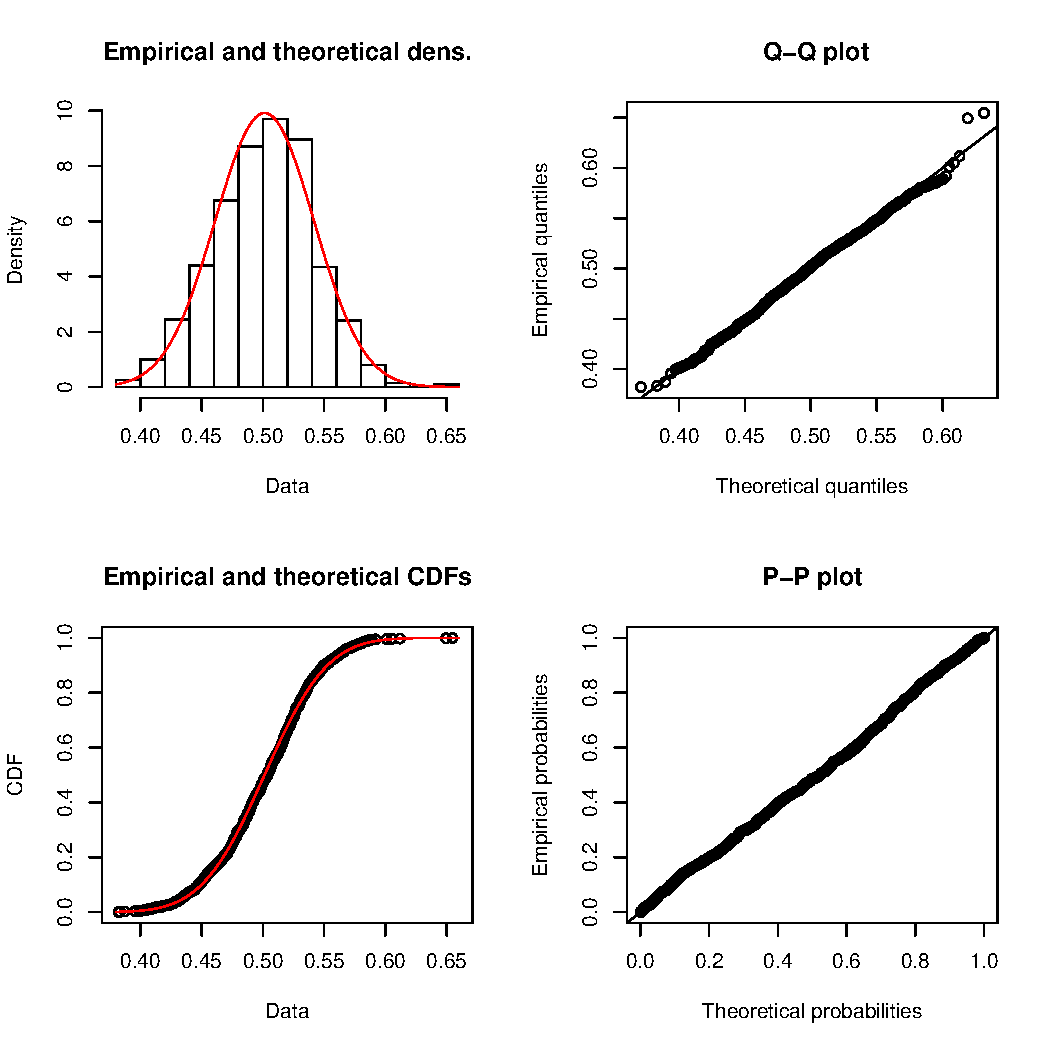
\includegraphics{2016_w09_files/figure-latex/unnamed-chunk-9-10.pdf}
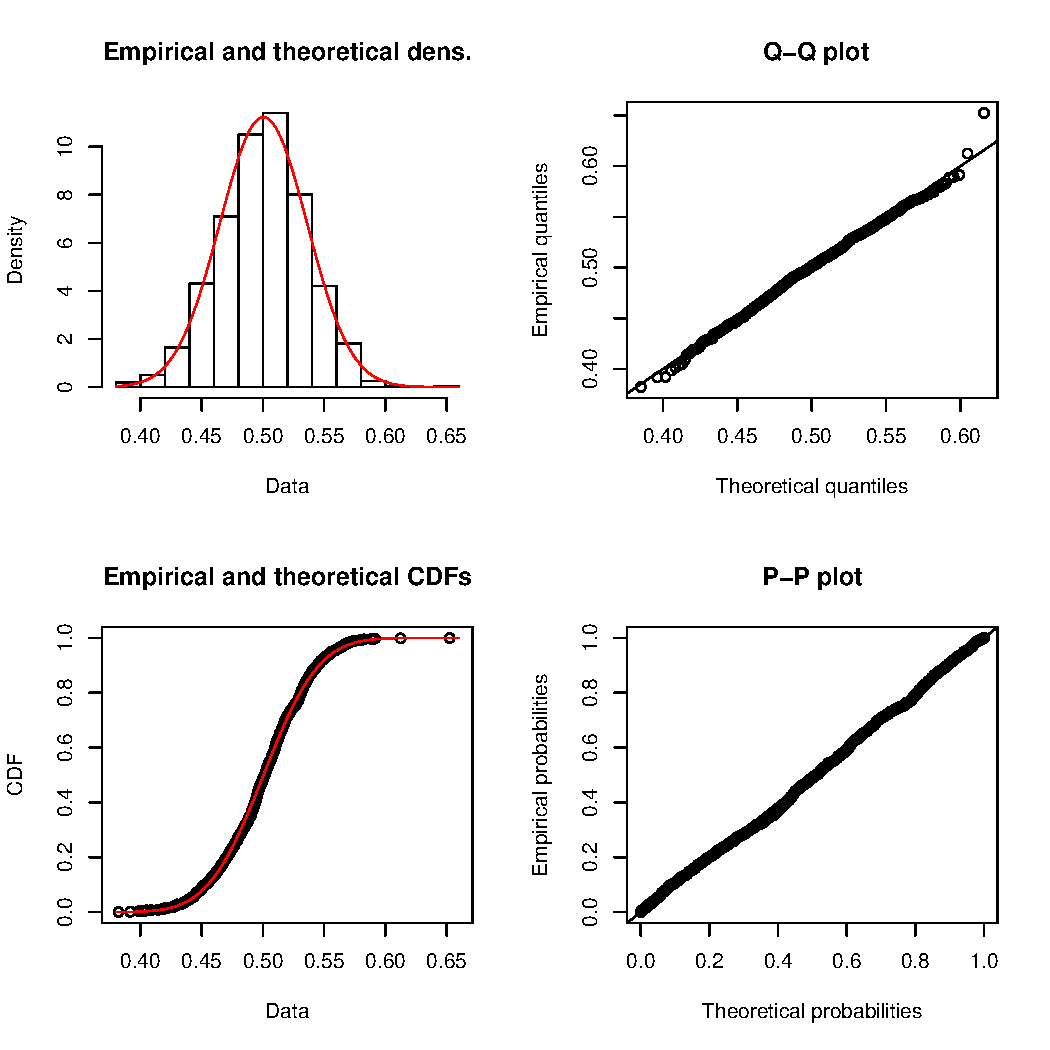
\includegraphics{2016_w09_files/figure-latex/unnamed-chunk-9-11.pdf}
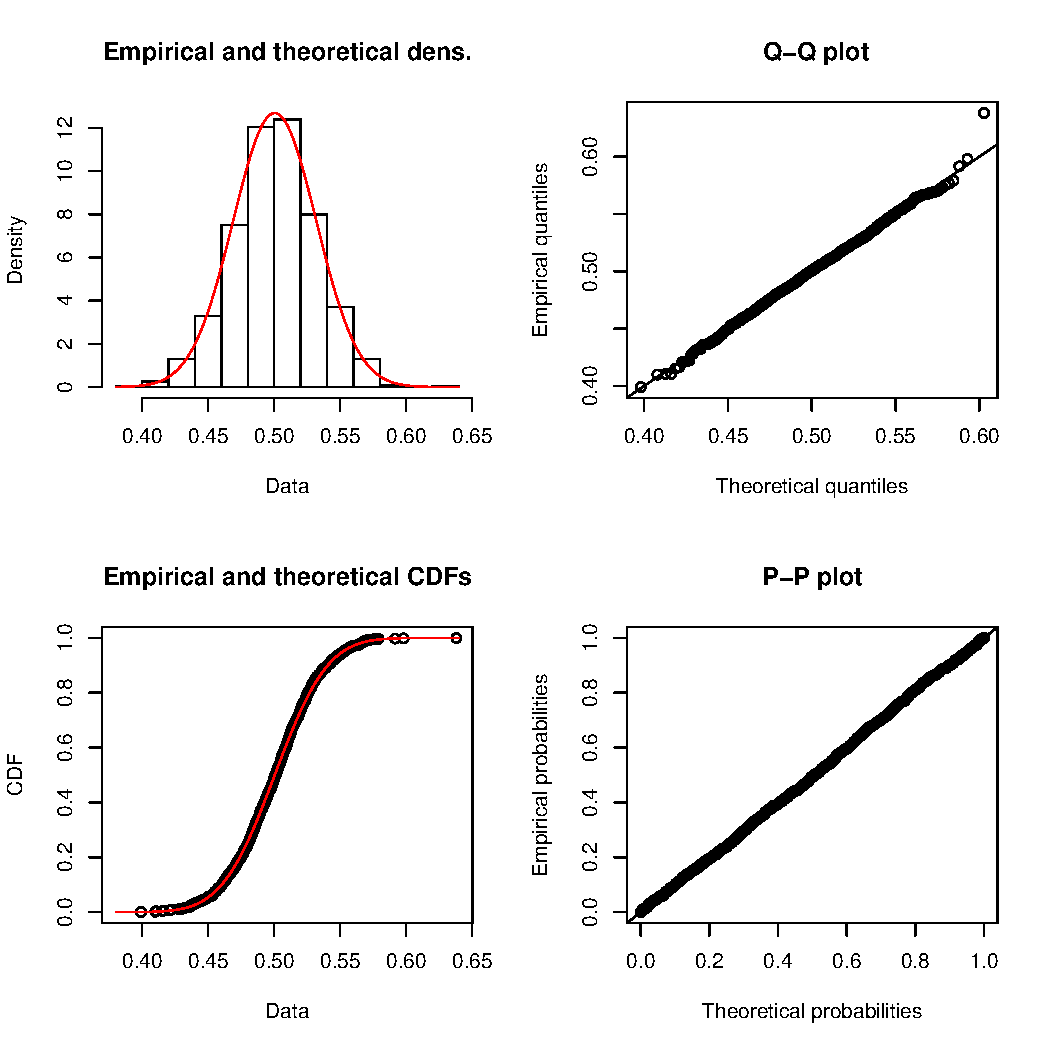
\includegraphics{2016_w09_files/figure-latex/unnamed-chunk-9-12.pdf}

Vid första anblick tycks det här som att den vanliga betafördelningen
trots allt kanske kan passa någorlunda? (Dock inte för alltför små n!)

\begin{itemize}
\tightlist
\item
  Finns det ngn systematik i hur shape1 och shape2 skattas utifrån n?
  Hade vart jättenitressant i så fall!
\item
  Kan vi använda dessa betafördelningar och jämföra mot den ickecentrala
  betafördelning pss som ovan?
\end{itemize}

\section{2016-03-02}\label{section-2}

Fortsätter leka lite med paketet \texttt{fitdistrplus}

\subsection{Testar att modifera beta-funktionerna för att också skatta
ncp
(misslyckas)}\label{testar-att-modifera-beta-funktionerna-for-att-ocksa-skatta-ncp-misslyckas}

\begin{Shaded}
\begin{Highlighting}[]
\NormalTok{pbeta <-}\StringTok{ }\NormalTok{function(q, shape1, shape2, }\DataTypeTok{ncp =} \DecValTok{0}\NormalTok{, }\DataTypeTok{lower.tail =} \OtherTok{TRUE}\NormalTok{, }\DataTypeTok{log.p =} \OtherTok{FALSE}\NormalTok{) }
  \KeywordTok{.Call}\NormalTok{(C_pnbeta, q, shape1, shape2, ncp, lower.tail, log.p)}
\NormalTok{dbeta <-}\StringTok{ }\NormalTok{function(x, shape1, shape2, }\DataTypeTok{ncp =} \DecValTok{0}\NormalTok{, }\DataTypeTok{log =} \OtherTok{FALSE}\NormalTok{)}
  \KeywordTok{.Call}\NormalTok{(C_dnbeta, x, shape1, shape2, ncp, log)}
\NormalTok{qbeta <-}\StringTok{ }\NormalTok{function(p, shape1, shape2, }\DataTypeTok{ncp =} \DecValTok{0}\NormalTok{, }\DataTypeTok{lower.tail =} \OtherTok{TRUE}\NormalTok{, }\DataTypeTok{log.p =} \OtherTok{FALSE}\NormalTok{)}
  \KeywordTok{.Call}\NormalTok{(C_qnbeta, p, shape1, shape2, ncp, lower.tail, log.p)}
\NormalTok{rbeta <-}\StringTok{ }\NormalTok{function(n, shape1, shape2, }\DataTypeTok{ncp =} \DecValTok{0}\NormalTok{) \{}
        \NormalTok{X <-}\StringTok{ }\KeywordTok{rchisq}\NormalTok{(n, }\DecValTok{2} \NormalTok{*}\StringTok{ }\NormalTok{shape1, }\DataTypeTok{ncp =} \NormalTok{ncp)}
        \NormalTok{X/(X +}\StringTok{ }\KeywordTok{rchisq}\NormalTok{(n, }\DecValTok{2} \NormalTok{*}\StringTok{ }\NormalTok{shape2))}
    \NormalTok{\}}
\KeywordTok{fitdist}\NormalTok{(R2[, }\DecValTok{1}\NormalTok{], }\StringTok{"beta"}\NormalTok{)}
\end{Highlighting}
\end{Shaded}

\begin{verbatim}
## Fitting of the distribution ' beta ' by maximum likelihood 
## Parameters:
##        estimate Std. Error
## shape1 1.823046 0.07720639
## shape2 1.881074 0.07998226
\end{verbatim}

Detta upprepades också med alla tillgängliga val av method men utan at
lyckas.

\subsection{Jämför resultat för olika
fördelningar}\label{jamfor-resultat-for-olika-fordelningar}

Vi har sett ovan att beta, gamma och normalfördelning kan funka för
olika stickprovsstorlekar. Vi kan undersöka detta.

\begin{Shaded}
\begin{Highlighting}[]
\KeywordTok{par}\NormalTok{(}\DataTypeTok{mfrow =} \KeywordTok{c}\NormalTok{(}\DecValTok{3}\NormalTok{, }\DecValTok{3}\NormalTok{))}
\NormalTok{plot.legend <-}\StringTok{ }\KeywordTok{c}\NormalTok{(}\StringTok{"beta"}\NormalTok{, }\StringTok{"gamma"}\NormalTok{, }\StringTok{"normal"}\NormalTok{)}
\NormalTok{fitdists <-}\StringTok{ }\NormalTok{function(x, }\DataTypeTok{distr =} \KeywordTok{c}\NormalTok{(}\StringTok{"beta"}\NormalTok{, }\StringTok{"gamma"}\NormalTok{, }\StringTok{"norm"}\NormalTok{)) }
  \KeywordTok{lapply}\NormalTok{(distr, function(d) }\KeywordTok{fitdist}\NormalTok{(x, d))}

\NormalTok{denscomps <-}\StringTok{ }\NormalTok{function(m, }\DataTypeTok{distr =} \KeywordTok{c}\NormalTok{(}\StringTok{"beta"}\NormalTok{, }\StringTok{"gamma"}\NormalTok{, }\StringTok{"norm"}\NormalTok{), ...) \{}
  \NormalTok{R2 <-}\StringTok{ }\KeywordTok{as.data.frame}\NormalTok{(m$Rsquared)}
  \KeywordTok{lapply}\NormalTok{(R2, function(r2) \{}
    \KeywordTok{denscomp}\NormalTok{(}\KeywordTok{fitdists}\NormalTok{(r2, }\DataTypeTok{distr =} \NormalTok{distr), ...)}
    \KeywordTok{abline}\NormalTok{(}\DataTypeTok{v =} \KeywordTok{attr}\NormalTok{(m, }\StringTok{"real_Rsquared"}\NormalTok{), }\DataTypeTok{col =} \StringTok{"blue"}\NormalTok{)}
  \NormalTok{\})}
\NormalTok{\}}
\KeywordTok{denscomps}\NormalTok{(m, }\DataTypeTok{legendtext =} \NormalTok{plot.legend)}
\end{Highlighting}
\end{Shaded}

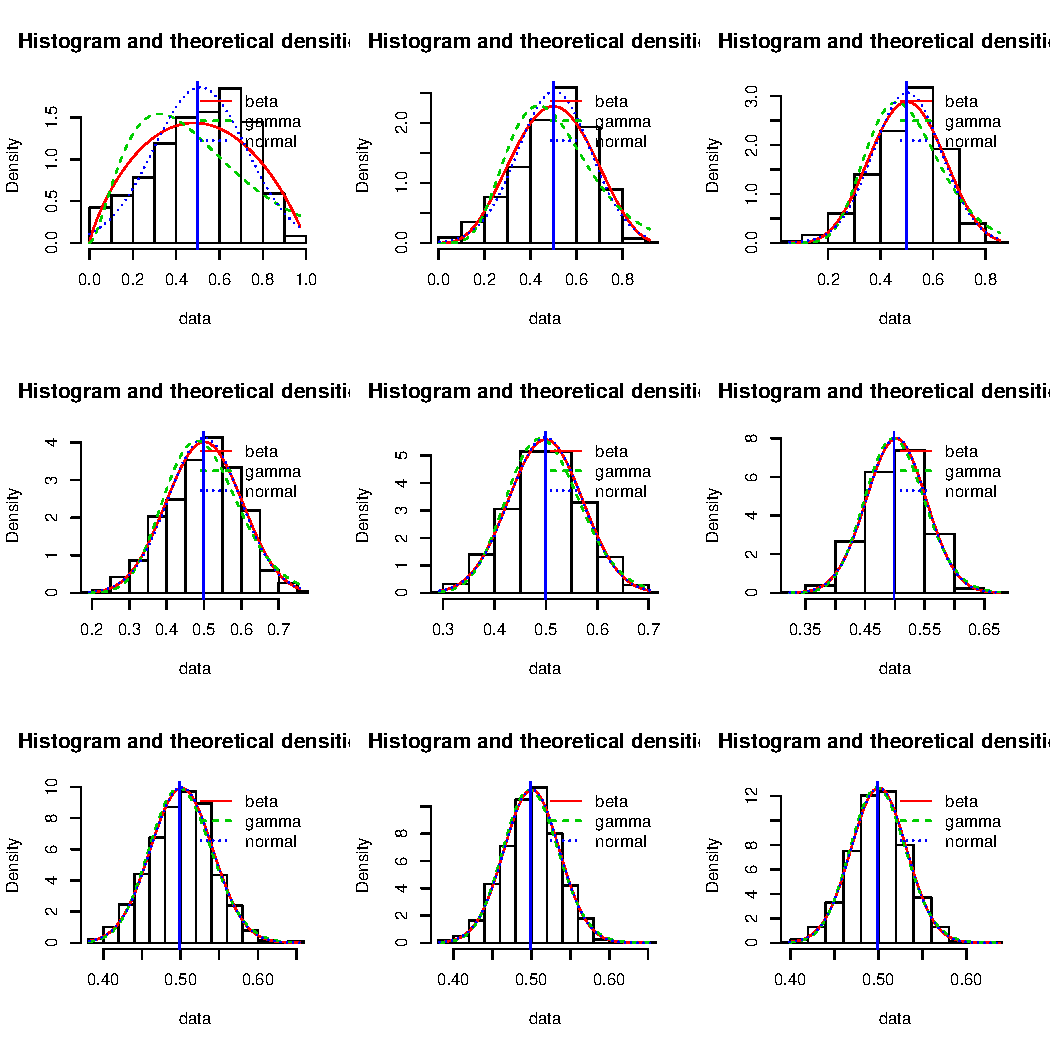
\includegraphics{2016_w09_files/figure-latex/unnamed-chunk-11-1.pdf}

\begin{verbatim}
## $`10`
## NULL
## 
## $`20`
## NULL
## 
## $`30`
## NULL
## 
## $`50`
## NULL
## 
## $`100`
## NULL
## 
## $`200`
## NULL
## 
## $`300`
## NULL
## 
## $`400`
## NULL
## 
## $`500`
## NULL
\end{verbatim}

Käns som att vi efter detta ganska klart kan förkasta gammafördelningen
som lämpli kandidat men kanske att den ändå skulle passa bättre för
mindre \(\rho\) (då den ju har en pos eskevhet).

\textbf{OBS!} Denna chunk sparas för att kunna härleda vad som gjort men
ej visat sig fruktsamt. Koden ska inte behöva anropas etc på nytt!

\begin{Shaded}
\begin{Highlighting}[]
\NormalTok{distplots <-}\StringTok{ }\NormalTok{function(}\DataTypeTok{r2 =} \NormalTok{.}\DecValTok{2}\NormalTok{, }\DataTypeTok{p =} \DecValTok{1}\NormalTok{) \{}
  \NormalTok{ss <-}\StringTok{ }\KeywordTok{sim_data}\NormalTok{(}\DataTypeTok{r2 =} \NormalTok{r2, }\DataTypeTok{p =} \NormalTok{p) %>%}\StringTok{ }
\StringTok{    }\KeywordTok{subsamples}\NormalTok{(}\DataTypeTok{n.max =} \DecValTok{500}\NormalTok{, }\DataTypeTok{N =} \DecValTok{1000}\NormalTok{)}
  \NormalTok{m <-}\StringTok{ }\KeywordTok{metrics}\NormalTok{(ss, }\DataTypeTok{n.sample =} \KeywordTok{c}\NormalTok{(}\DecValTok{10}\NormalTok{, }\DecValTok{20}\NormalTok{, }\DecValTok{30}\NormalTok{, }\DecValTok{50}\NormalTok{, }\DecValTok{100}\NormalTok{, }\DecValTok{200}\NormalTok{, }\DecValTok{300}\NormalTok{, }\DecValTok{400}\NormalTok{, }\DecValTok{500}\NormalTok{))}
  \KeywordTok{denscomps}\NormalTok{(m, }\DataTypeTok{legendtext =} \NormalTok{plot.legend)}
\NormalTok{\}}

\KeywordTok{par}\NormalTok{(}\DataTypeTok{mfrow =} \KeywordTok{c}\NormalTok{(}\DecValTok{3}\NormalTok{, }\DecValTok{3}\NormalTok{))}
\KeywordTok{lapply}\NormalTok{(}\KeywordTok{c}\NormalTok{(.}\DecValTok{2}\NormalTok{, .}\DecValTok{5}\NormalTok{, .}\DecValTok{8}\NormalTok{), distplots)}
\end{Highlighting}
\end{Shaded}

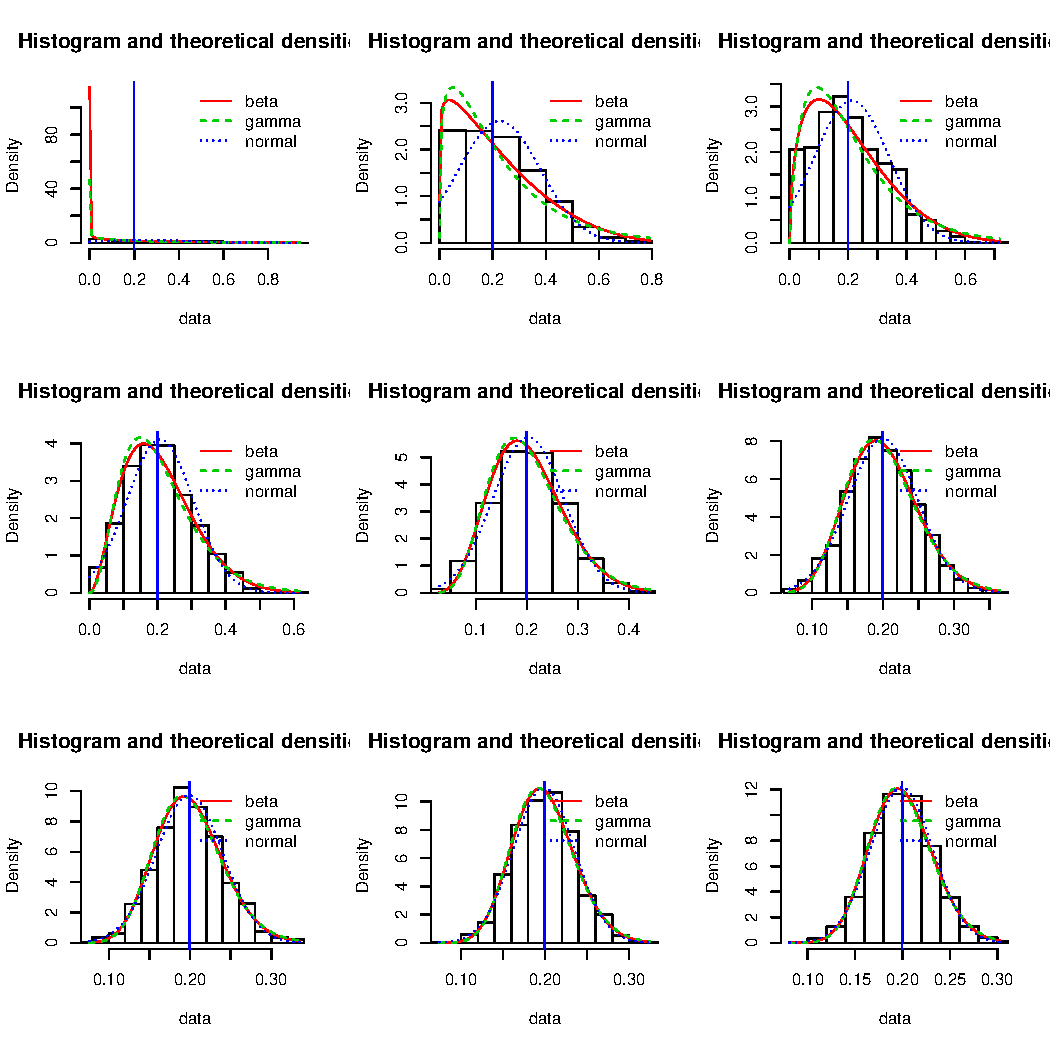
\includegraphics{2016_w09_files/figure-latex/unnamed-chunk-12-1.pdf}
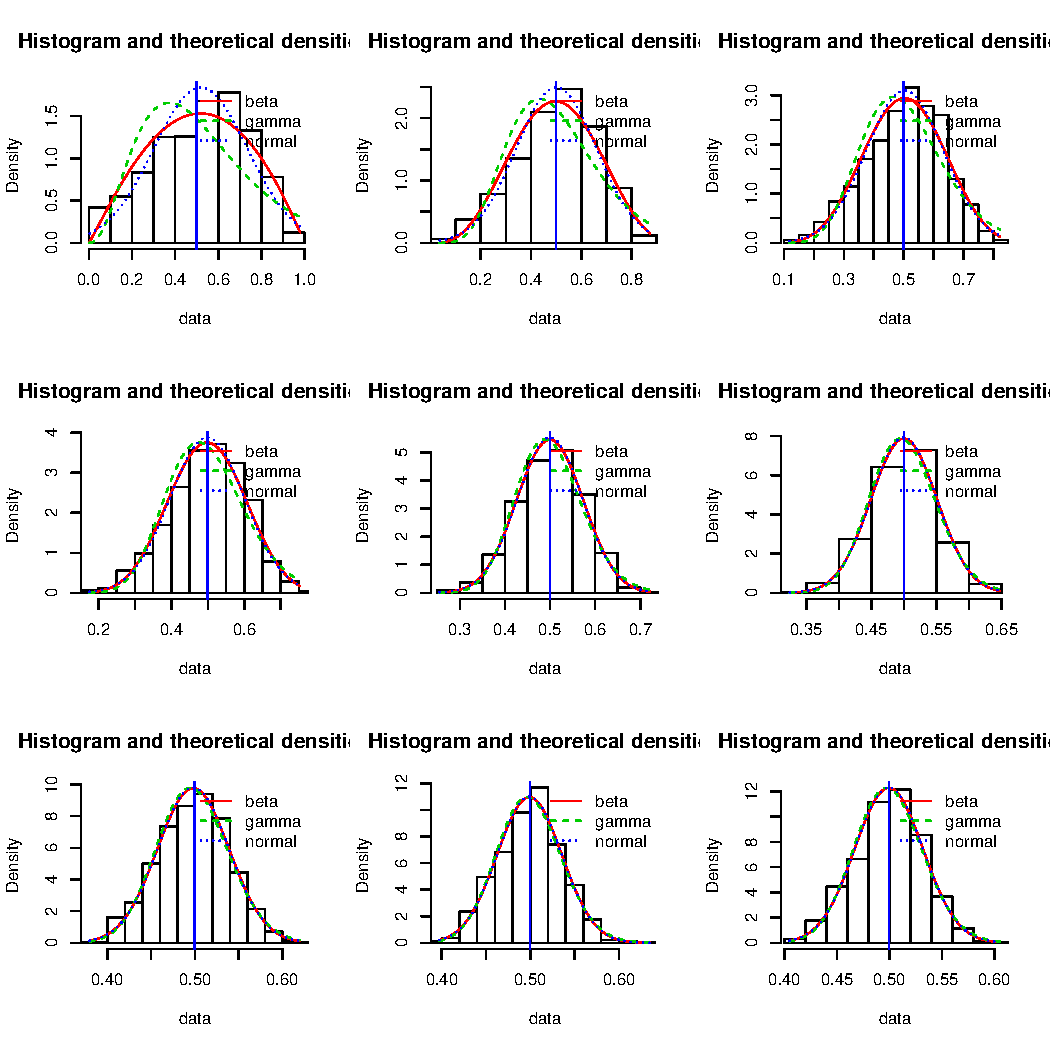
\includegraphics{2016_w09_files/figure-latex/unnamed-chunk-12-2.pdf}
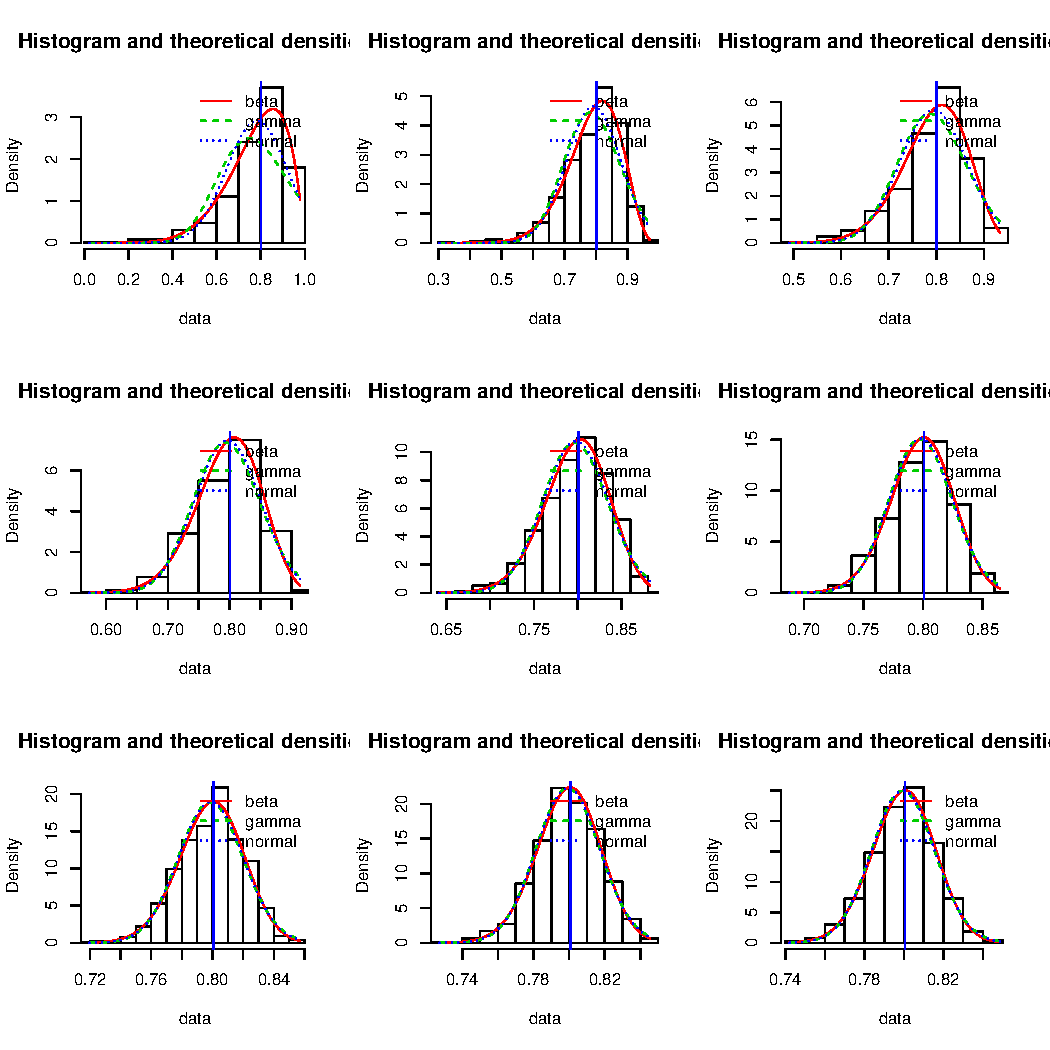
\includegraphics{2016_w09_files/figure-latex/unnamed-chunk-12-3.pdf}
Finner att gamma de facto passar bättre för just små \(\rho\) men att
beta ändå är ett bättre alternativ. Ser därmed ingen anledning att
fortsätta studera gamma-fördelningen i detta sammanhang. Ser också att
resultaten är ganska samstämmiga för \(n> 200\) så begränsar mig dit men
tar istället in lite fler mellanliggande värden som kanske kan vara
intressanta. Värjer mig nu heller inte för att ta ännu fler \(\rho\).

\begin{Shaded}
\begin{Highlighting}[]
\NormalTok{distplots <-}\StringTok{ }\NormalTok{function(}\DataTypeTok{r2 =} \NormalTok{.}\DecValTok{2}\NormalTok{, }\DataTypeTok{p =} \DecValTok{1}\NormalTok{, }\DataTypeTok{distr =} \KeywordTok{c}\NormalTok{(}\StringTok{"beta"}\NormalTok{, }\StringTok{"norm"}\NormalTok{), }
                      \DataTypeTok{n.sample =} \KeywordTok{c}\NormalTok{(}\DecValTok{5}\NormalTok{, }\DecValTok{10}\NormalTok{, }\DecValTok{20}\NormalTok{, }\DecValTok{30}\NormalTok{, }\DecValTok{50}\NormalTok{, }\DecValTok{75}\NormalTok{, }\DecValTok{100}\NormalTok{, }\DecValTok{150}\NormalTok{, }\DecValTok{200}\NormalTok{), ...) \{}
  \NormalTok{ss <-}\StringTok{ }\KeywordTok{sim_data}\NormalTok{(}\DataTypeTok{r2 =} \NormalTok{r2, }\DataTypeTok{p =} \NormalTok{p) %>%}\StringTok{ }
\StringTok{    }\KeywordTok{subsamples}\NormalTok{(}\DataTypeTok{n.max =} \KeywordTok{max}\NormalTok{(n.sample), }\DataTypeTok{N =} \DecValTok{1000}\NormalTok{)}
  \NormalTok{m <-}\StringTok{ }\KeywordTok{metrics}\NormalTok{(ss, }\DataTypeTok{n.sample =} \NormalTok{n.sample)}
  \KeywordTok{par}\NormalTok{(}\DataTypeTok{mfrow =} \KeywordTok{c}\NormalTok{(}\KeywordTok{floor}\NormalTok{(}\KeywordTok{sqrt}\NormalTok{(}\KeywordTok{length}\NormalTok{(n.sample))), }\KeywordTok{ceiling}\NormalTok{(}\KeywordTok{sqrt}\NormalTok{(}\KeywordTok{length}\NormalTok{(n.sample)))))}
  \KeywordTok{denscomps}\NormalTok{(m, }\DataTypeTok{distr =} \NormalTok{distr, }\DataTypeTok{legendtext =} \NormalTok{distr, }\DataTypeTok{main =} \KeywordTok{paste}\NormalTok{(}\StringTok{"rho = "}\NormalTok{, r2, }\StringTok{". p = "}\NormalTok{, p), ...)}
\NormalTok{\}}

\KeywordTok{lapply}\NormalTok{(}\KeywordTok{seq}\NormalTok{(}\DecValTok{0}\NormalTok{, .}\DecValTok{9}\NormalTok{, .}\DecValTok{1}\NormalTok{), distplots)}
\end{Highlighting}
\end{Shaded}

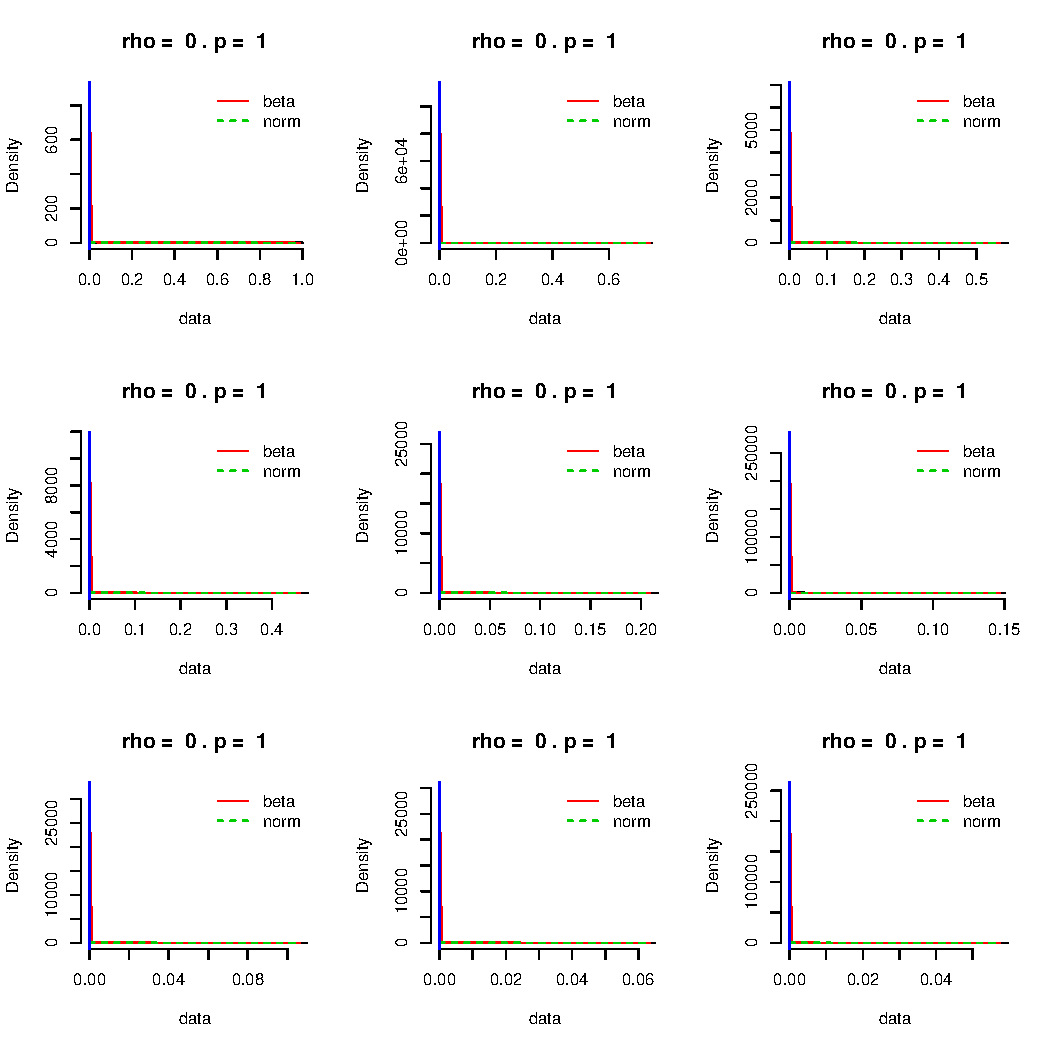
\includegraphics{2016_w09_files/figure-latex/unnamed-chunk-13-1.pdf}
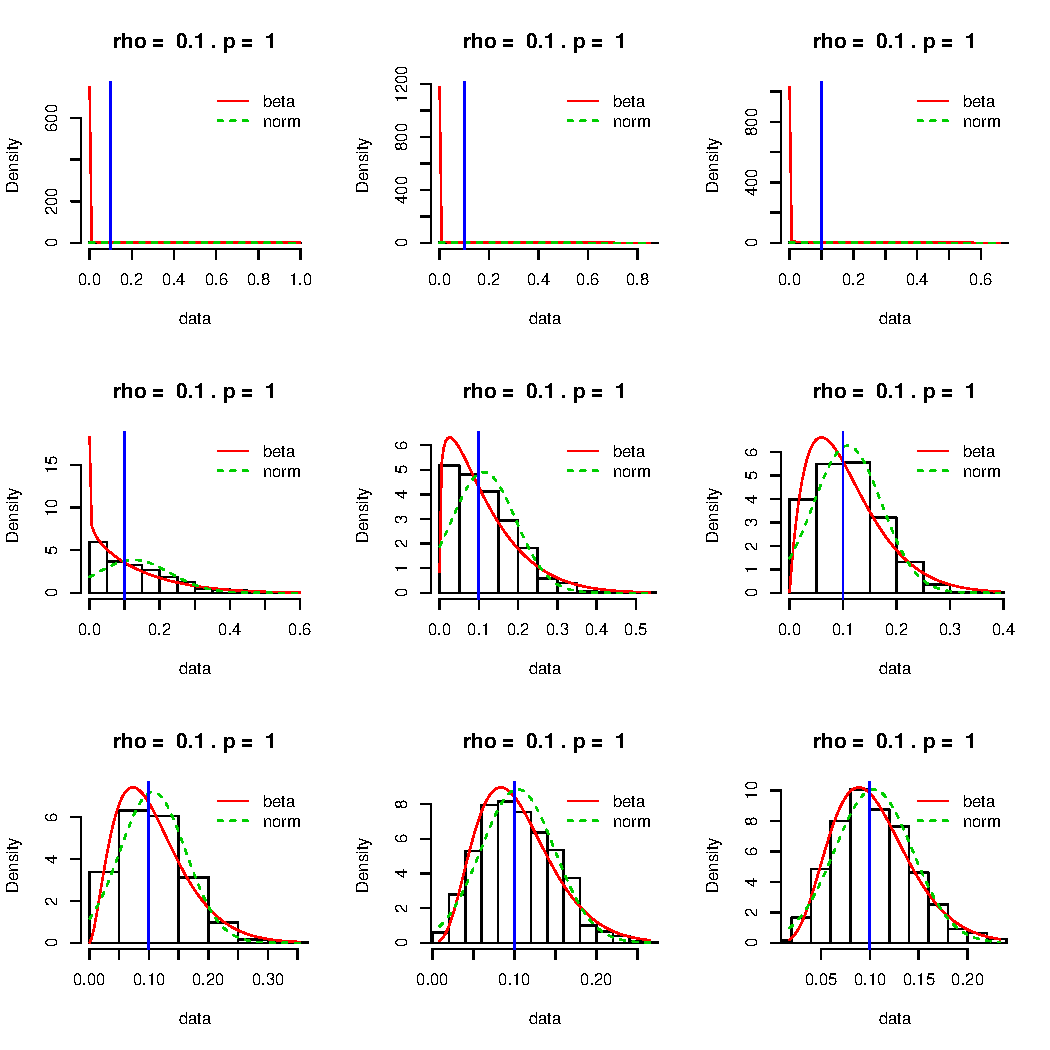
\includegraphics{2016_w09_files/figure-latex/unnamed-chunk-13-2.pdf}
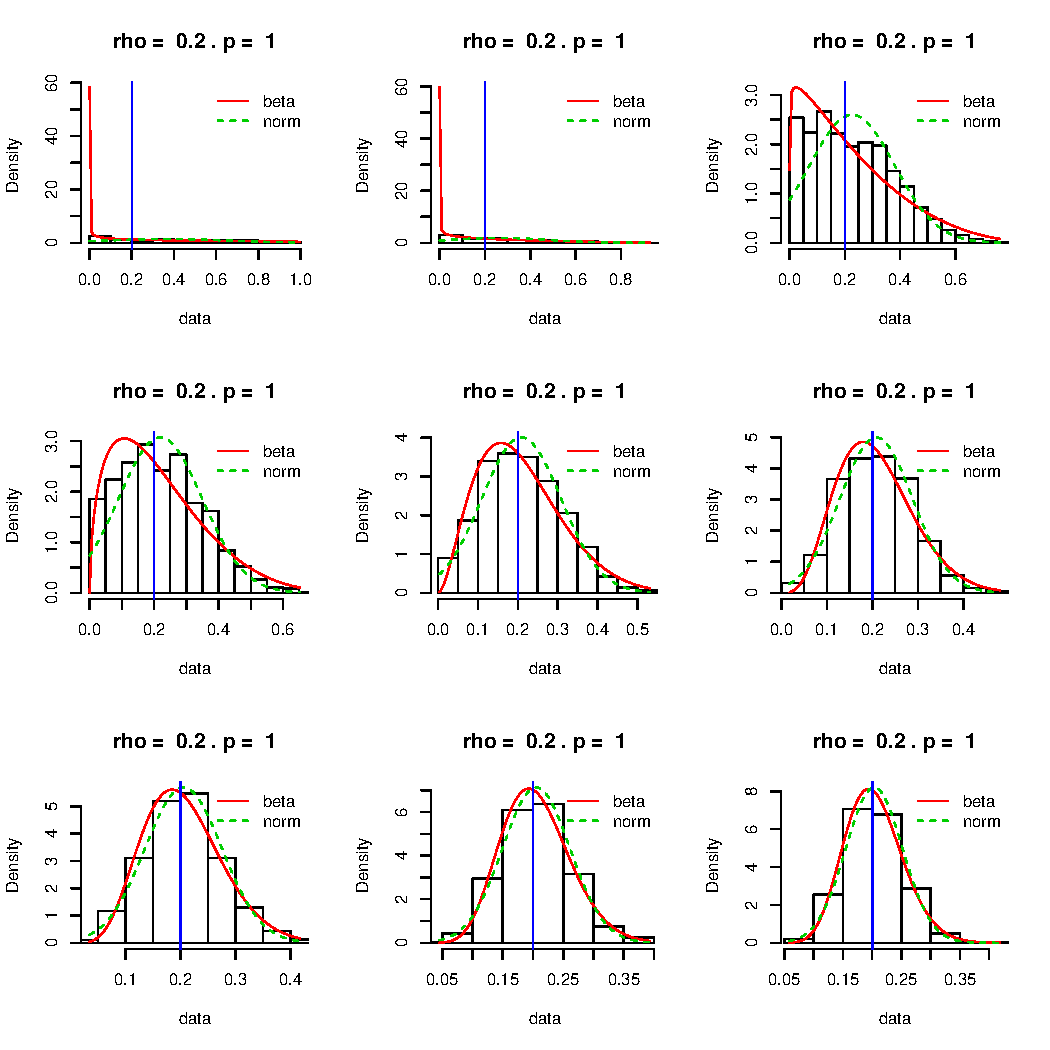
\includegraphics{2016_w09_files/figure-latex/unnamed-chunk-13-3.pdf}
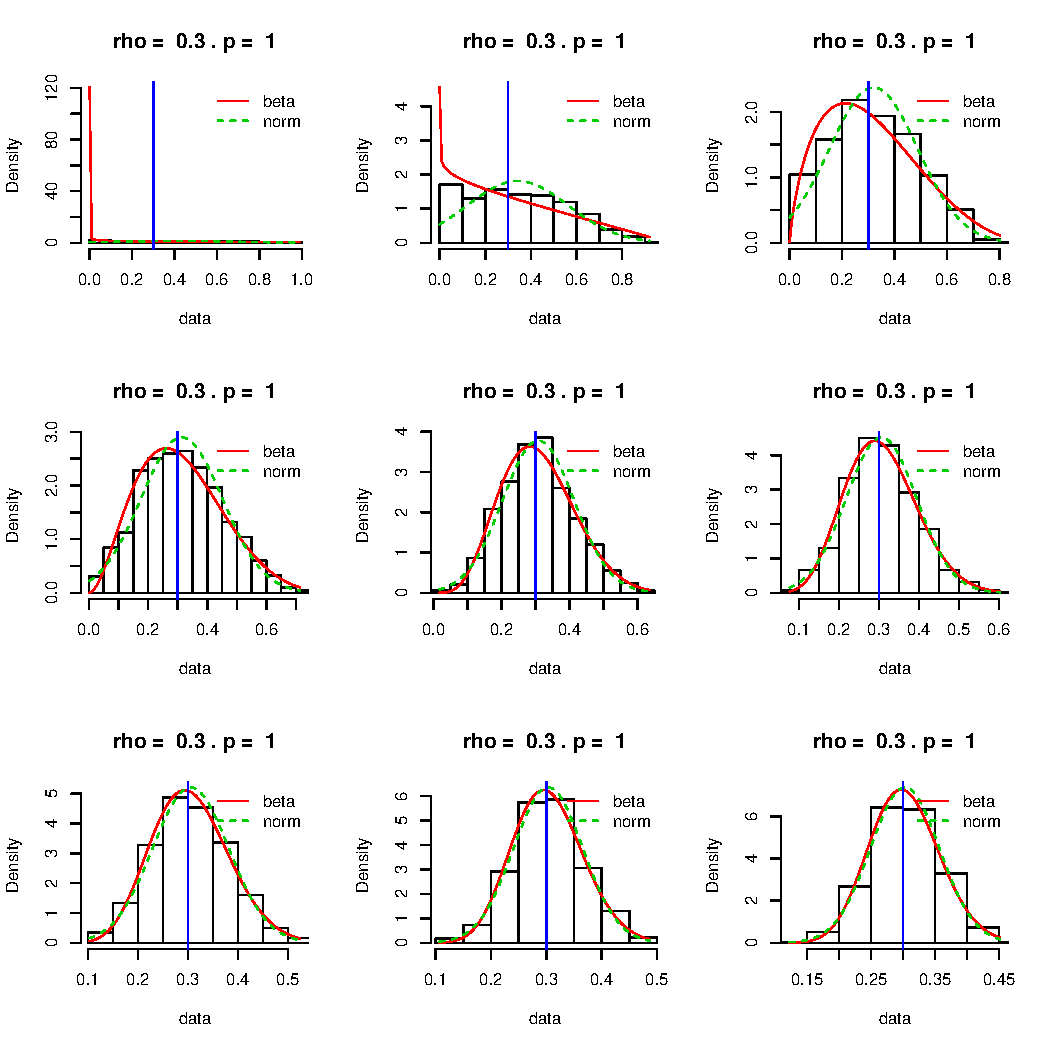
\includegraphics{2016_w09_files/figure-latex/unnamed-chunk-13-4.pdf}
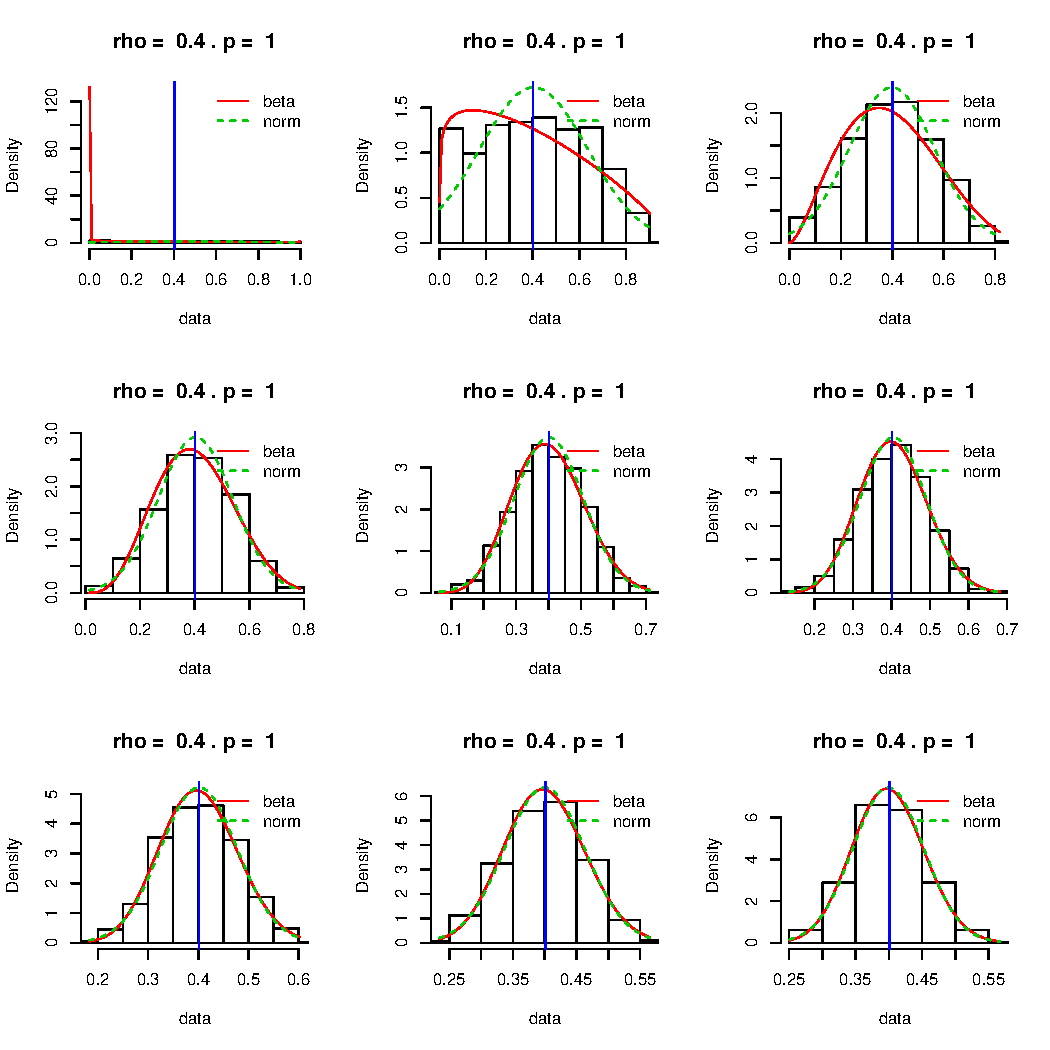
\includegraphics{2016_w09_files/figure-latex/unnamed-chunk-13-5.pdf}
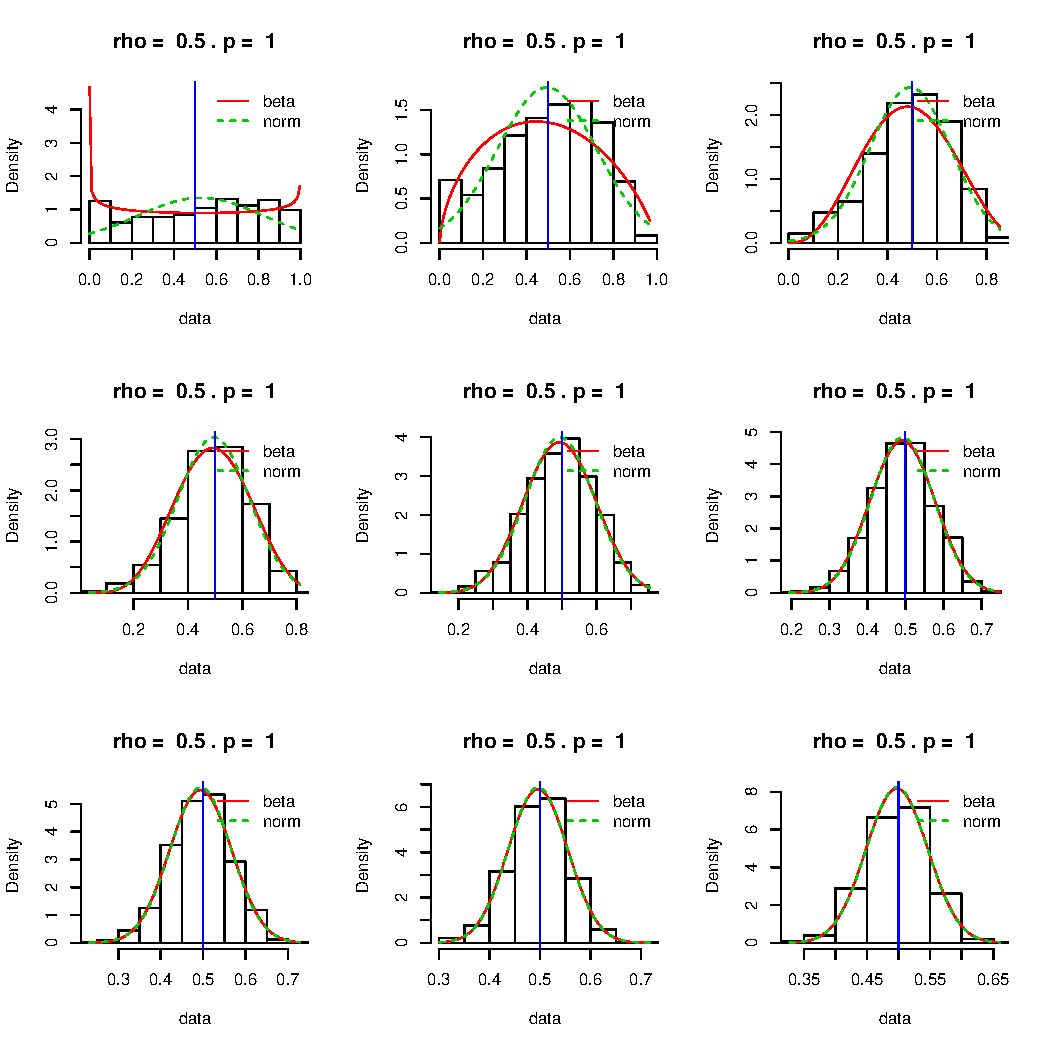
\includegraphics{2016_w09_files/figure-latex/unnamed-chunk-13-6.pdf}
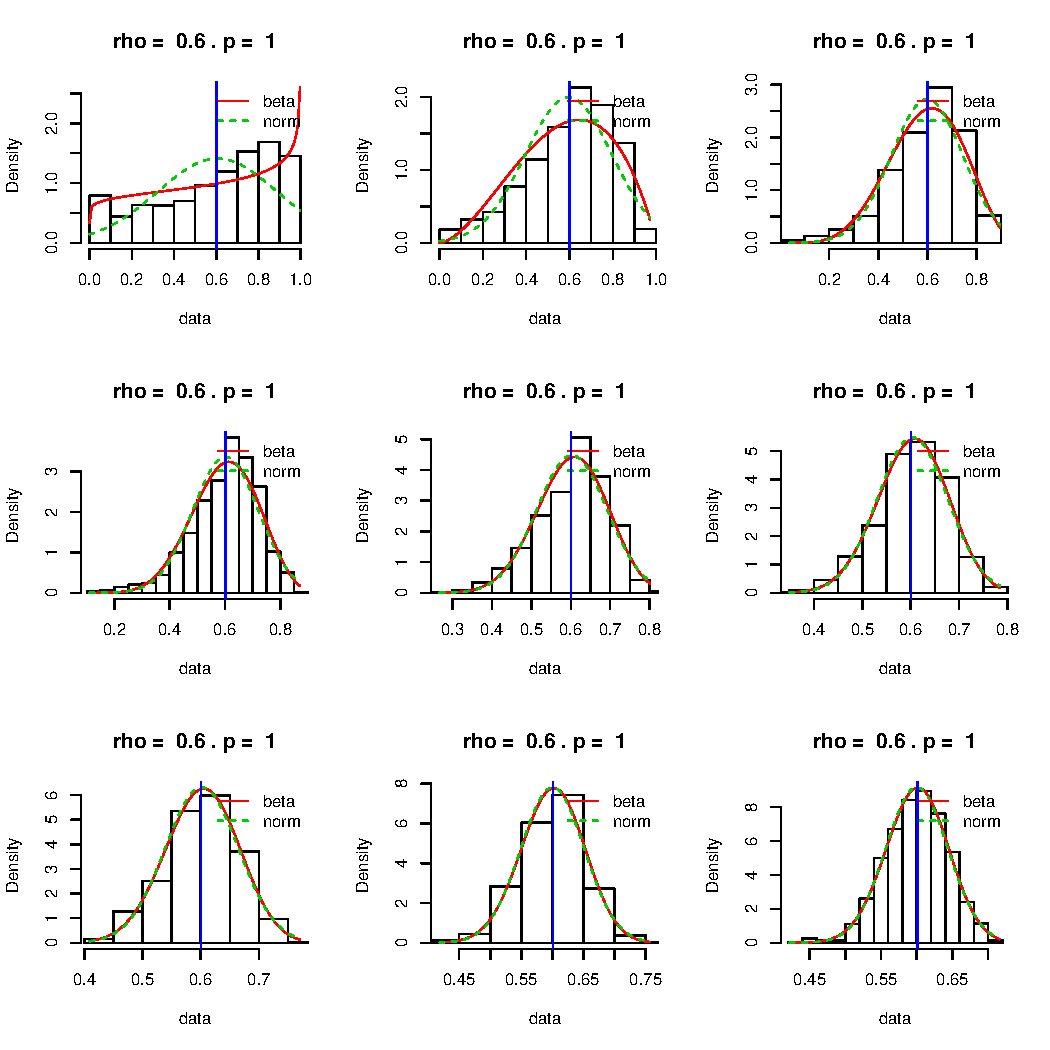
\includegraphics{2016_w09_files/figure-latex/unnamed-chunk-13-7.pdf}
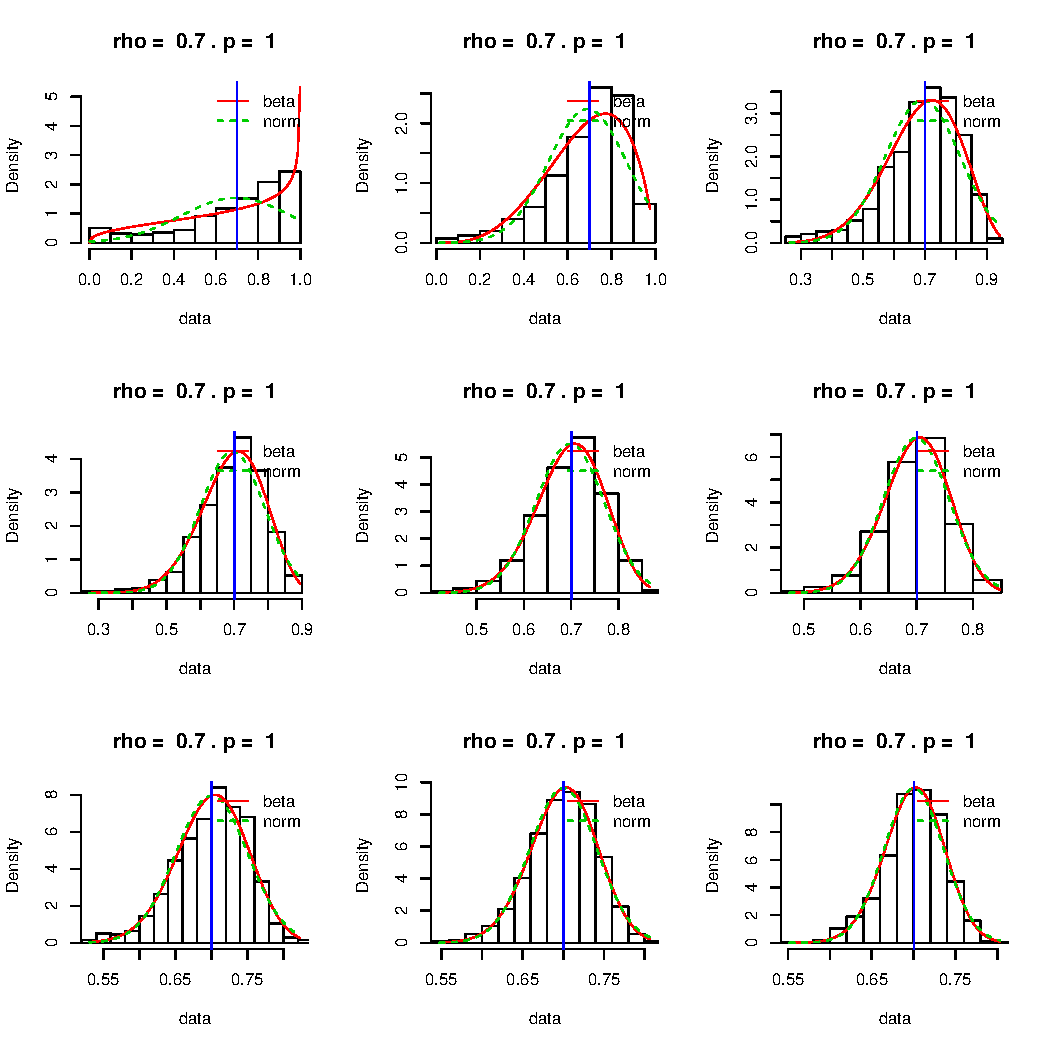
\includegraphics{2016_w09_files/figure-latex/unnamed-chunk-13-8.pdf}
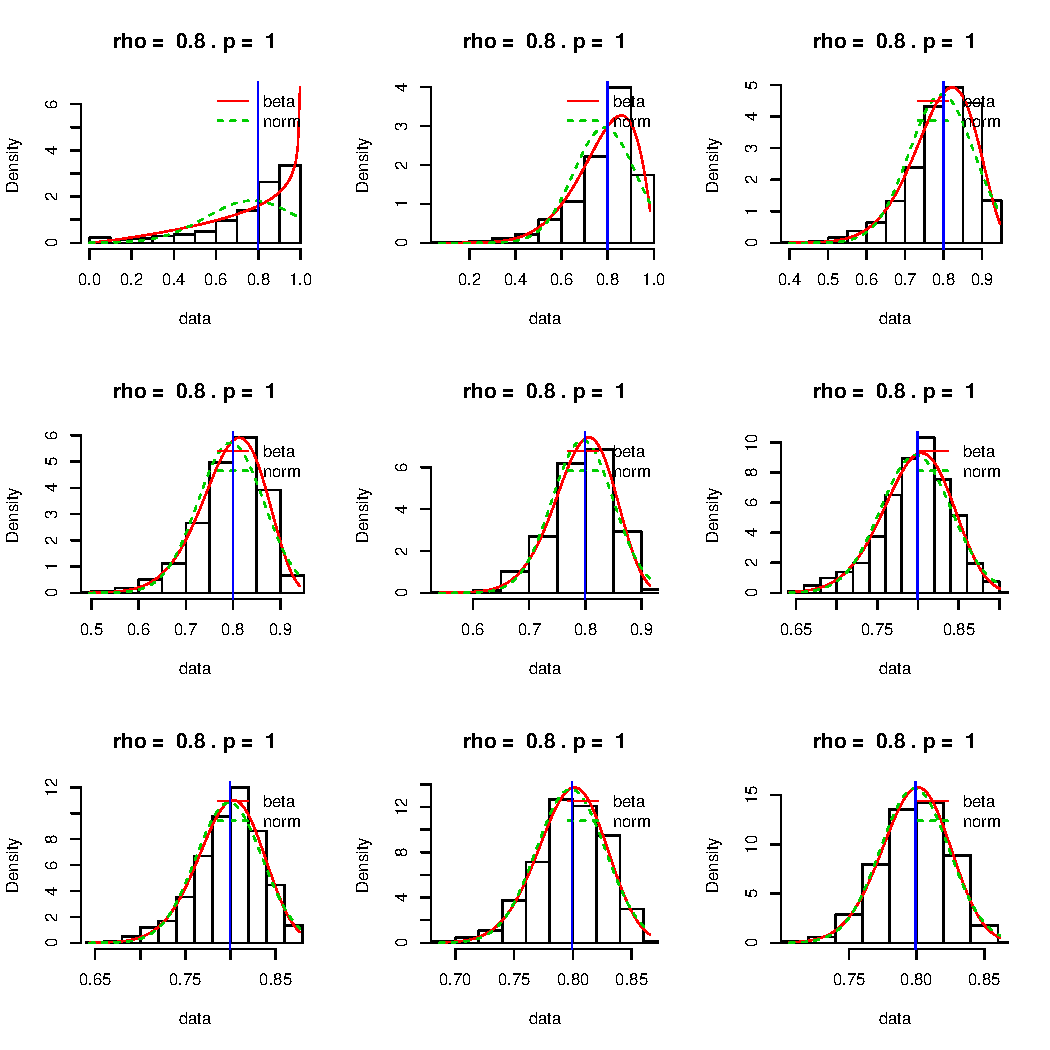
\includegraphics{2016_w09_files/figure-latex/unnamed-chunk-13-9.pdf}
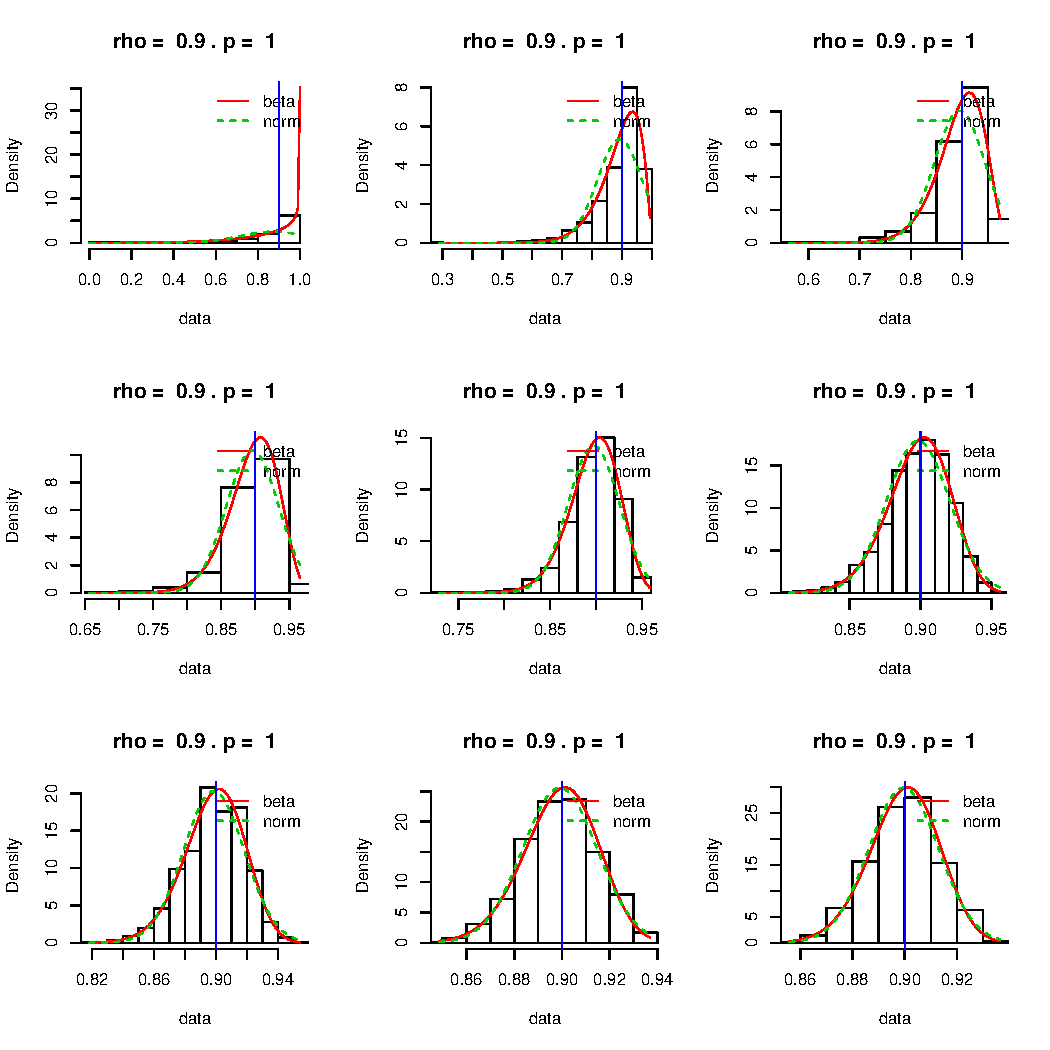
\includegraphics{2016_w09_files/figure-latex/unnamed-chunk-13-10.pdf}

\textbf{Slutsatser:} Vi kan se att beta-fördelningen ger alldeles för
höga skattningar för väldigt små \(\rho\). Problemet är alltså inte att
det inte blir några data men att y-axeln dras ut så mkt att dessa värden
inte syns. När \(\rho\) blir större blir det lättare att anpassa
fördelning ävendå \(n\) mindre. I några fall kan normalfördelningen
tyckas t o m bättre än beta men gissar att detta trots allt beror på
slumpen. När \(\rho\) dock ökar till att ligga närmare \(.5\) börjar
fördelningen krumbukta sig ganska ordentligt ör ökande \(n<20\). För
\(\rho > .6\) tycks det som att betafördelningen inte riktigt når upp
till högsta värdena i histogrammet. I detta avseende är t o m
normalfördelningen bättre. För \(n> 20\) tycks det dessutom som att beta
och normal är approximativt likvärdiga. Att högsta stapeln ligger över
betafördelningens mode tycks f.ö. hålla i sig för växande \(\rho\) men
effekten avtar med mindre \(n\) för ökade \(\rho\).

\subsection{För ökande p}\label{for-okande-p}

Vi vill också undersöka effekten om vi ökar antalet oberoende variabler
(p)

\subsubsection{p = 2}\label{p-2}

\begin{Shaded}
\begin{Highlighting}[]
\KeywordTok{lapply}\NormalTok{(}\KeywordTok{seq}\NormalTok{(}\DecValTok{0}\NormalTok{, .}\DecValTok{9}\NormalTok{, .}\DecValTok{1}\NormalTok{), distplots, }\DataTypeTok{p =} \DecValTok{2}\NormalTok{)}
\end{Highlighting}
\end{Shaded}

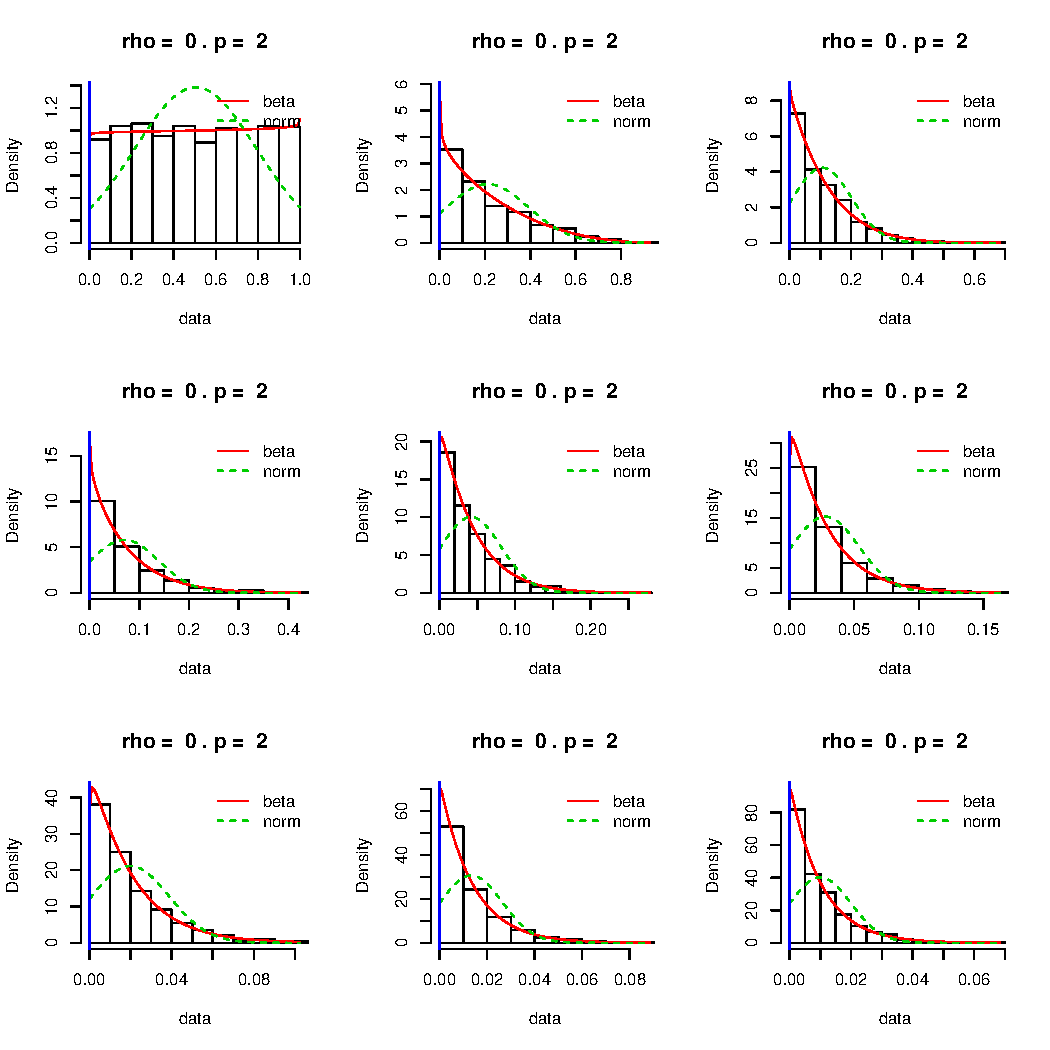
\includegraphics{2016_w09_files/figure-latex/unnamed-chunk-14-1.pdf}
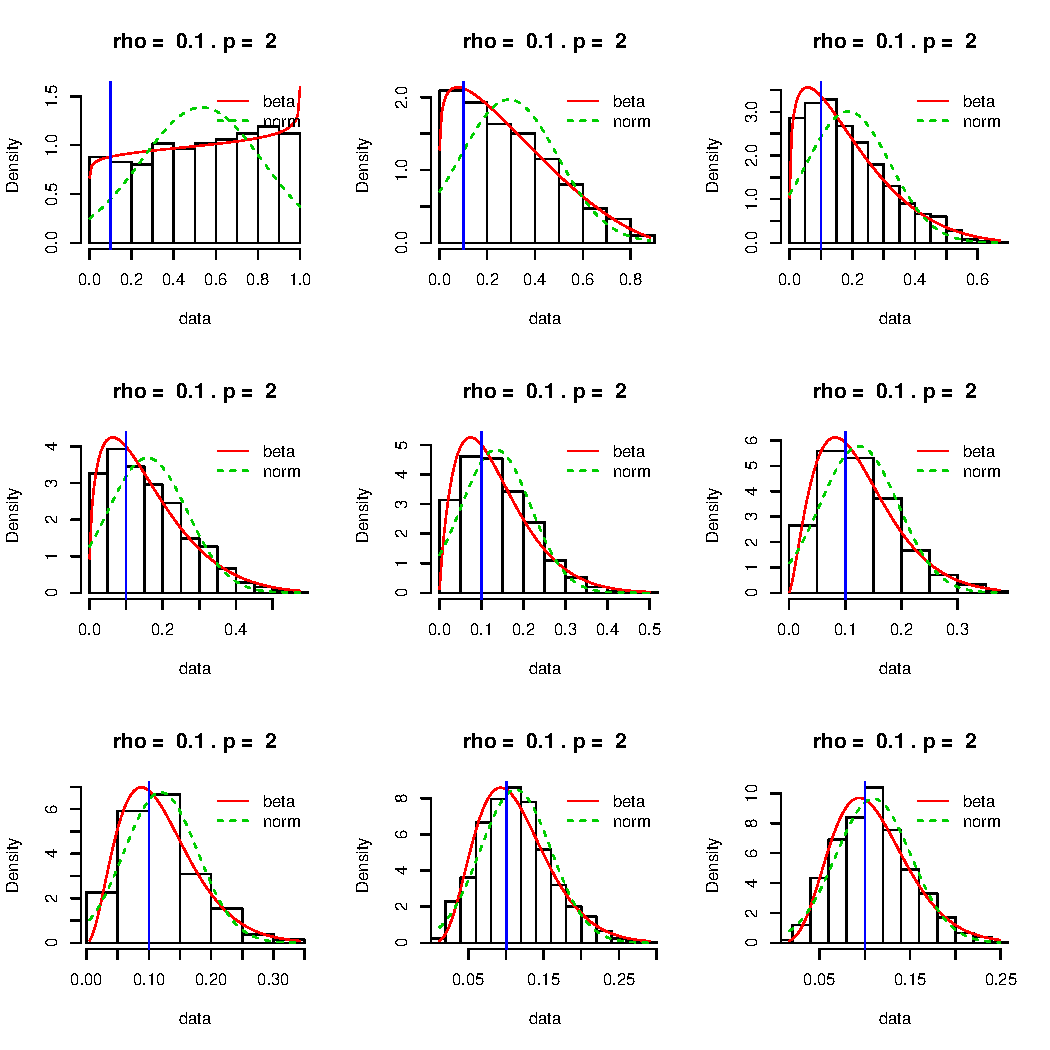
\includegraphics{2016_w09_files/figure-latex/unnamed-chunk-14-2.pdf}
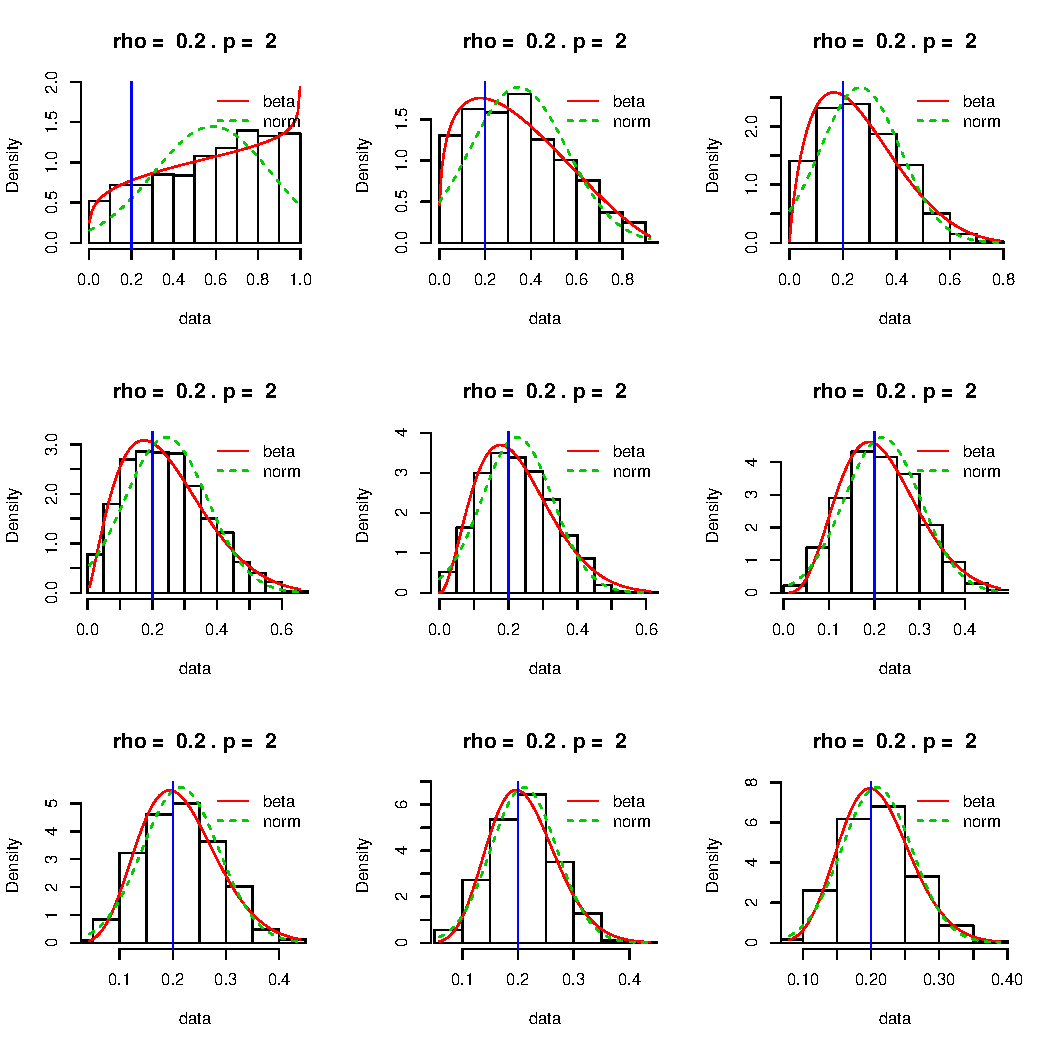
\includegraphics{2016_w09_files/figure-latex/unnamed-chunk-14-3.pdf}
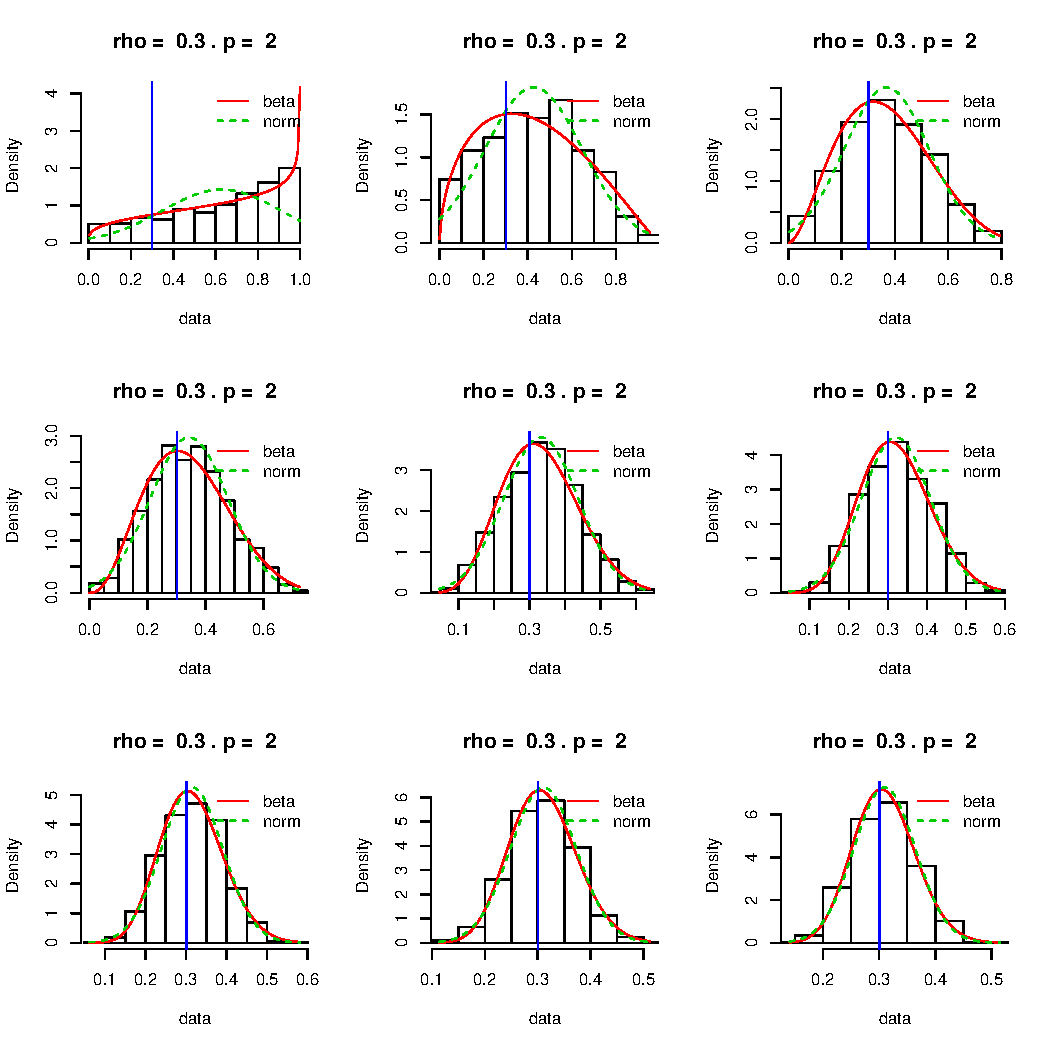
\includegraphics{2016_w09_files/figure-latex/unnamed-chunk-14-4.pdf}
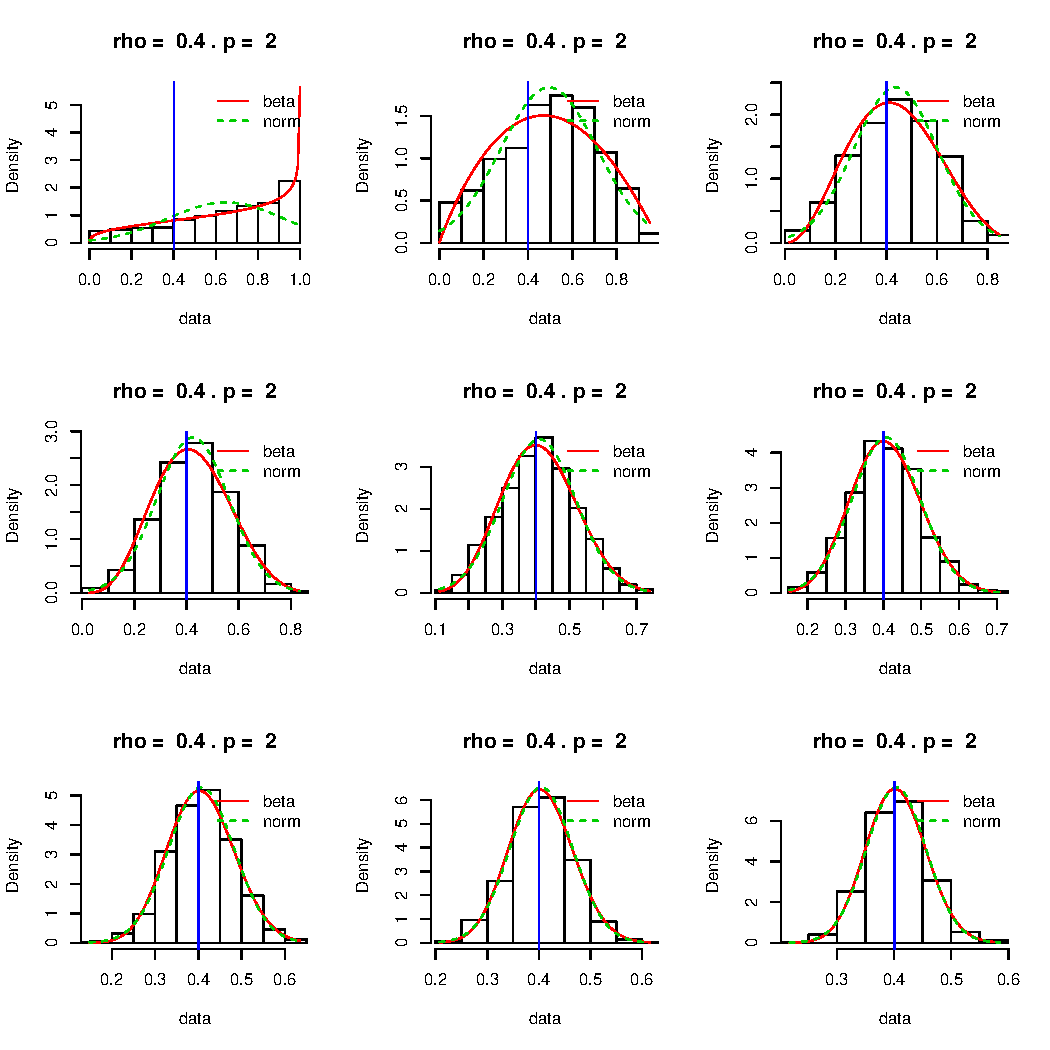
\includegraphics{2016_w09_files/figure-latex/unnamed-chunk-14-5.pdf}
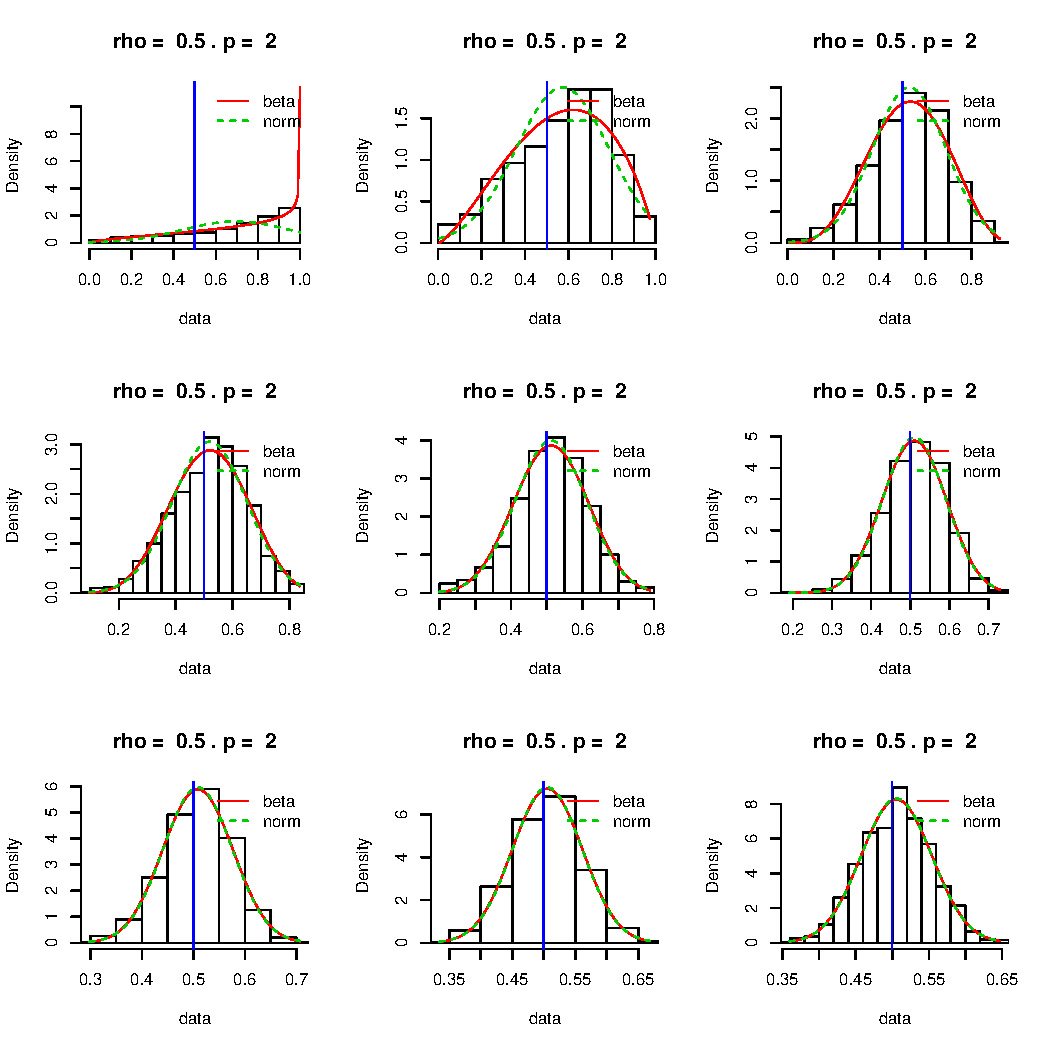
\includegraphics{2016_w09_files/figure-latex/unnamed-chunk-14-6.pdf}
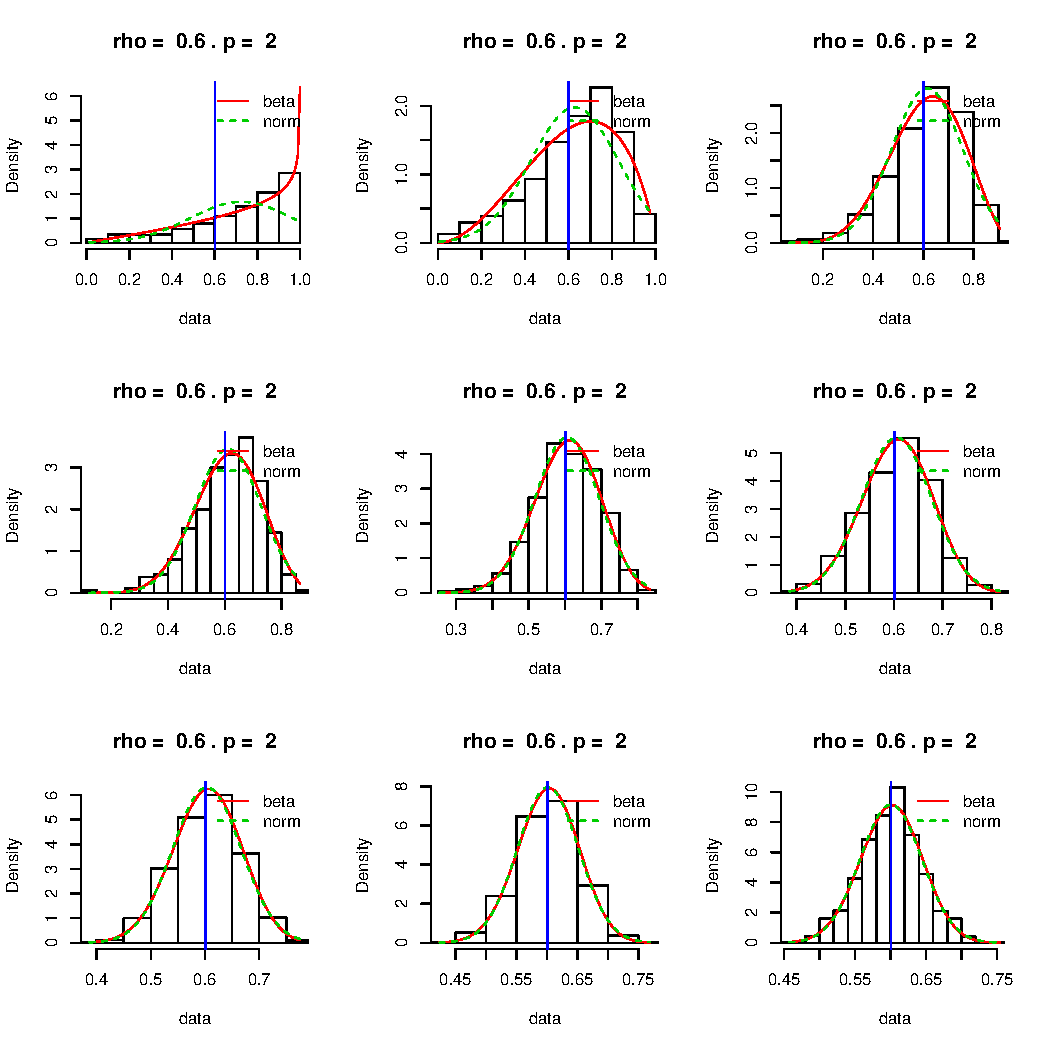
\includegraphics{2016_w09_files/figure-latex/unnamed-chunk-14-7.pdf}
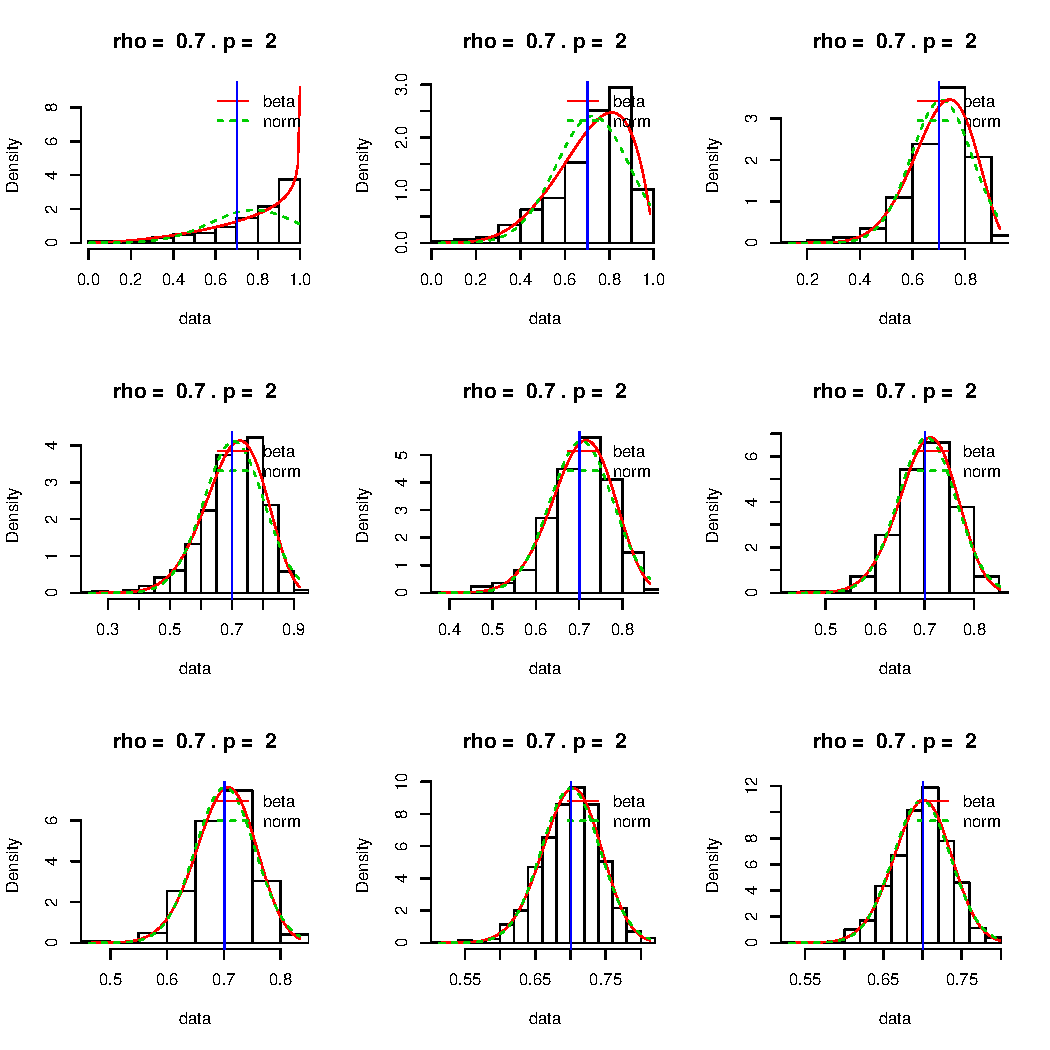
\includegraphics{2016_w09_files/figure-latex/unnamed-chunk-14-8.pdf}
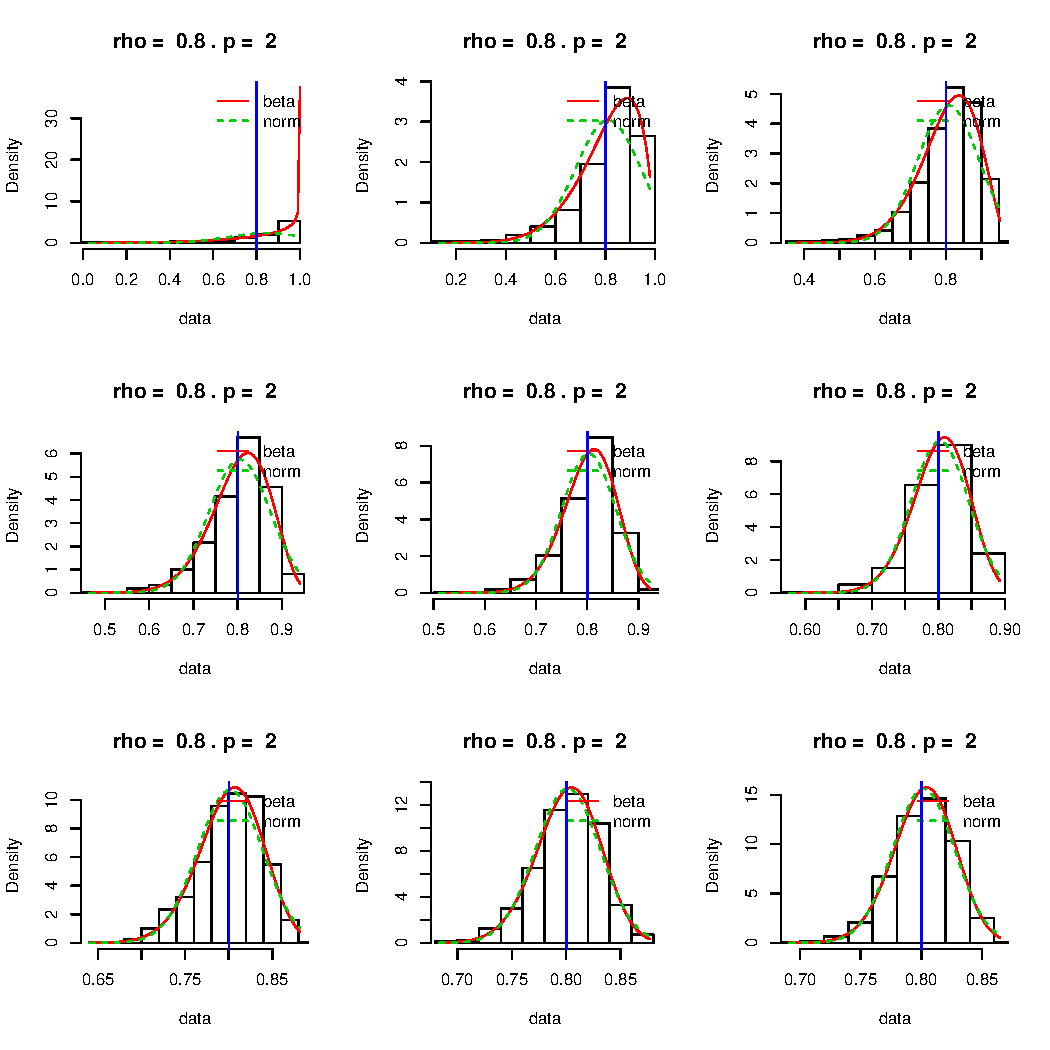
\includegraphics{2016_w09_files/figure-latex/unnamed-chunk-14-9.pdf}
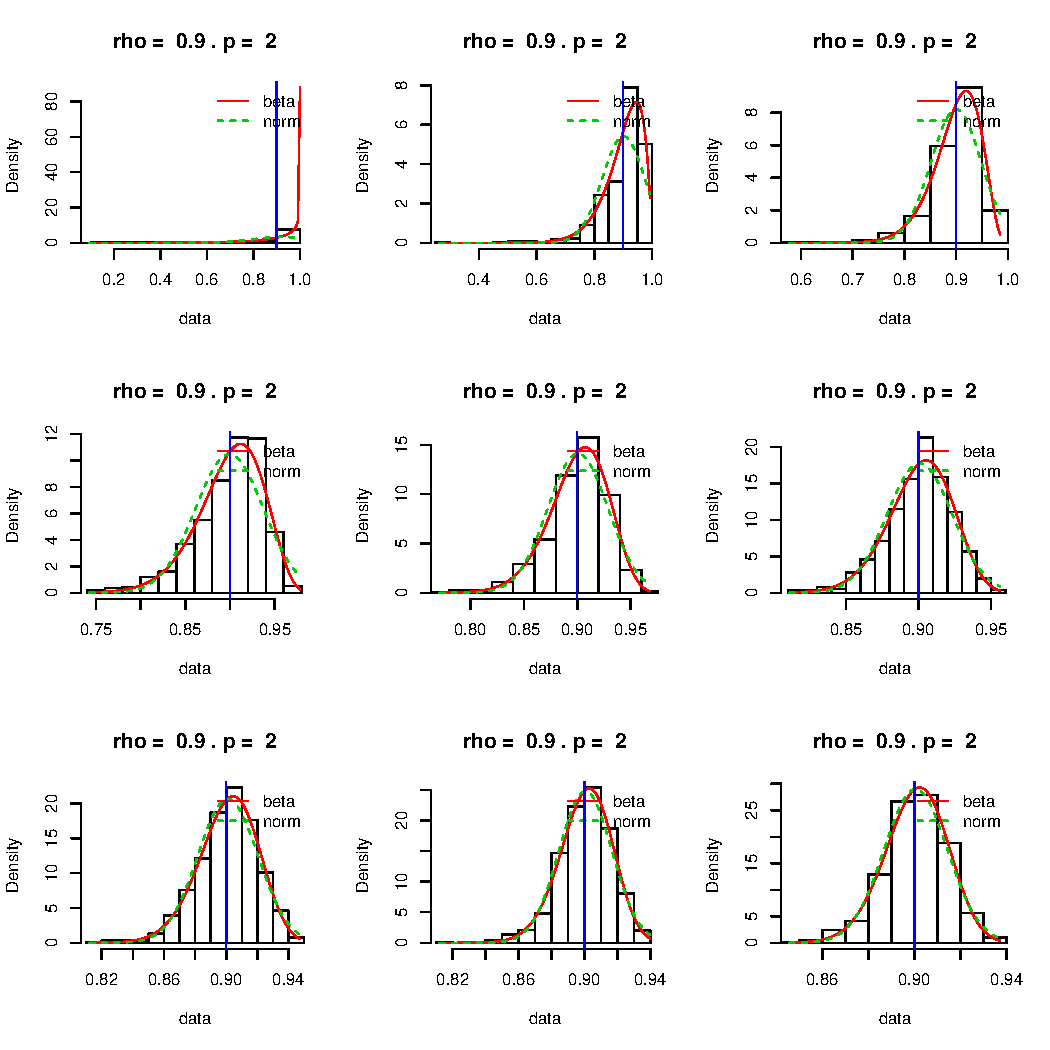
\includegraphics{2016_w09_files/figure-latex/unnamed-chunk-14-10.pdf}

\subsubsection{p = 3}\label{p-3}

\begin{Shaded}
\begin{Highlighting}[]
\KeywordTok{lapply}\NormalTok{(}\KeywordTok{seq}\NormalTok{(}\DecValTok{0}\NormalTok{, .}\DecValTok{9}\NormalTok{, .}\DecValTok{1}\NormalTok{), distplots, }\DataTypeTok{p =} \DecValTok{3}\NormalTok{)}
\end{Highlighting}
\end{Shaded}

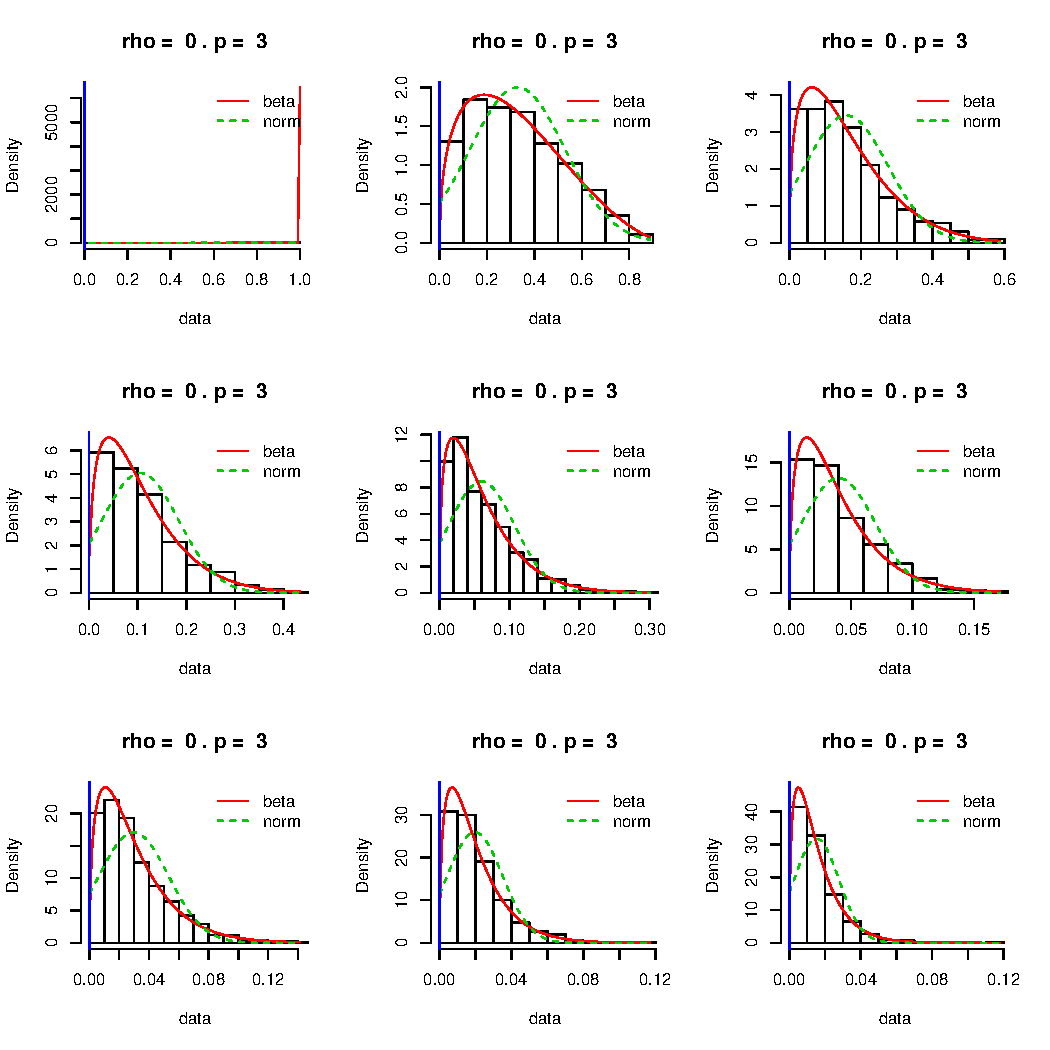
\includegraphics{2016_w09_files/figure-latex/unnamed-chunk-15-1.pdf}
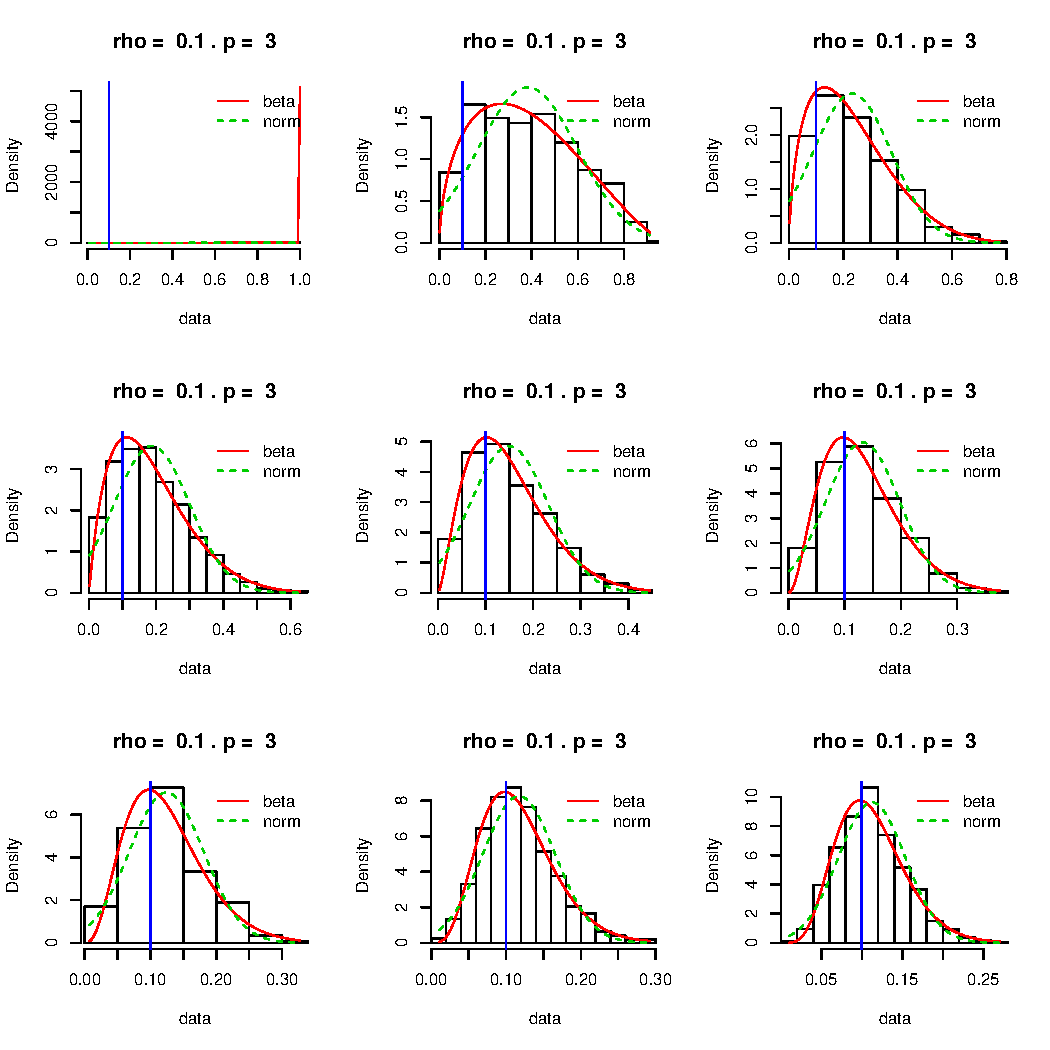
\includegraphics{2016_w09_files/figure-latex/unnamed-chunk-15-2.pdf}
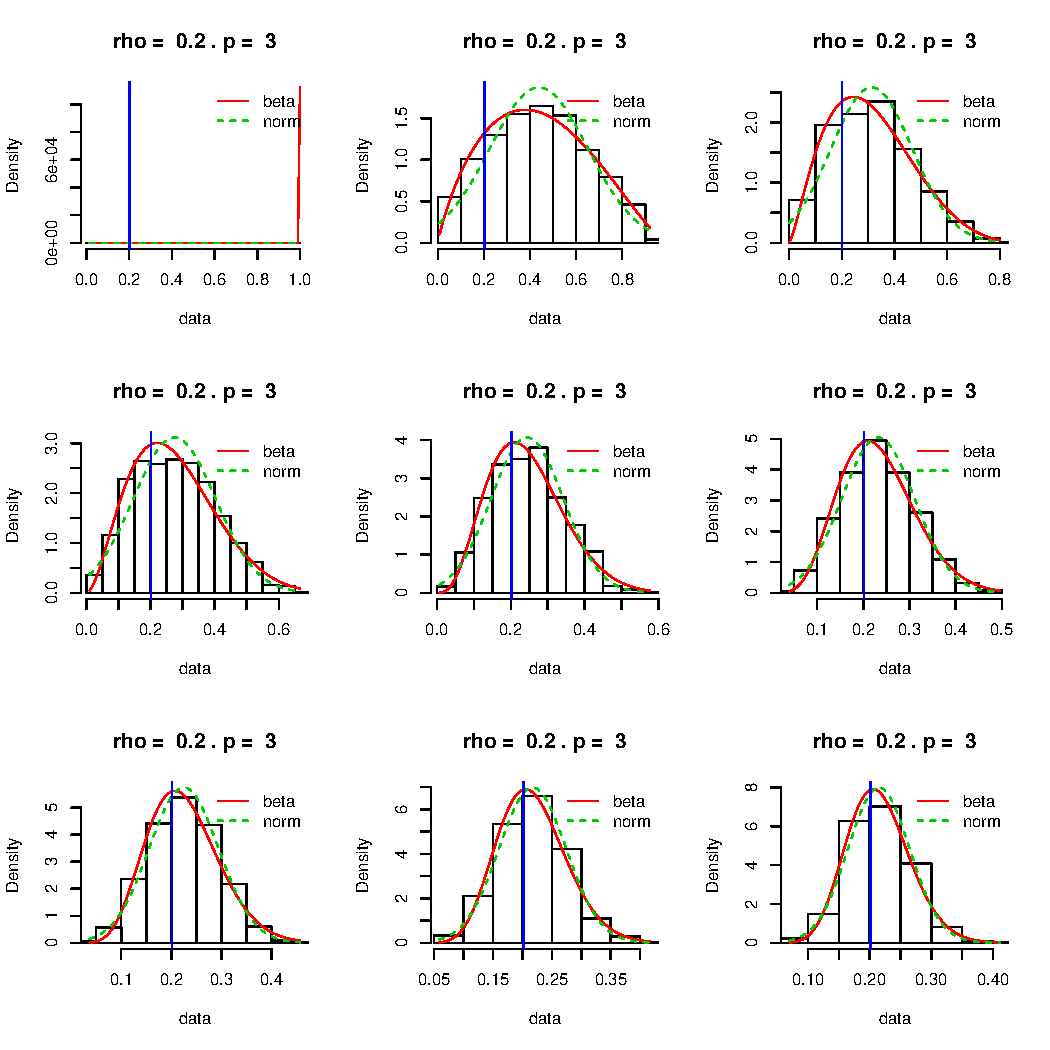
\includegraphics{2016_w09_files/figure-latex/unnamed-chunk-15-3.pdf}
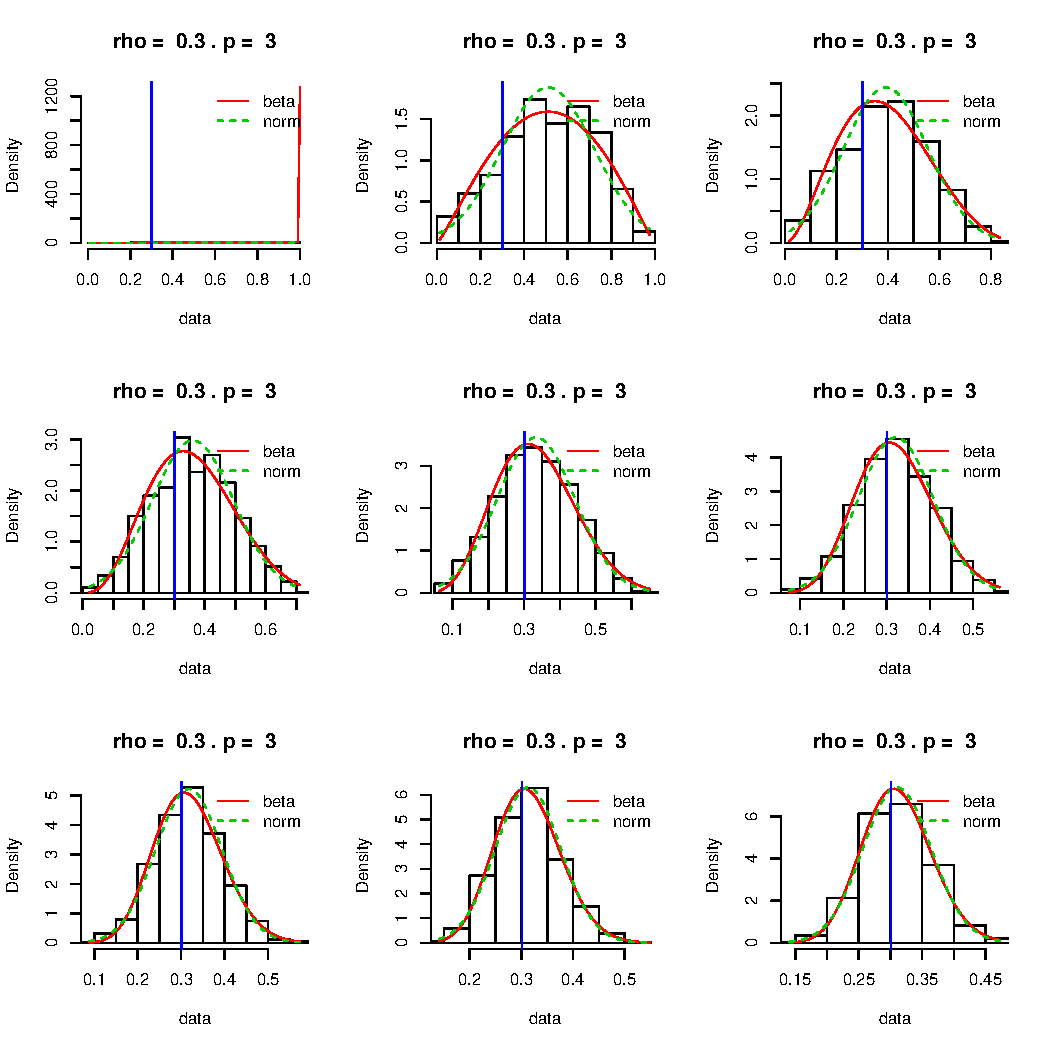
\includegraphics{2016_w09_files/figure-latex/unnamed-chunk-15-4.pdf}
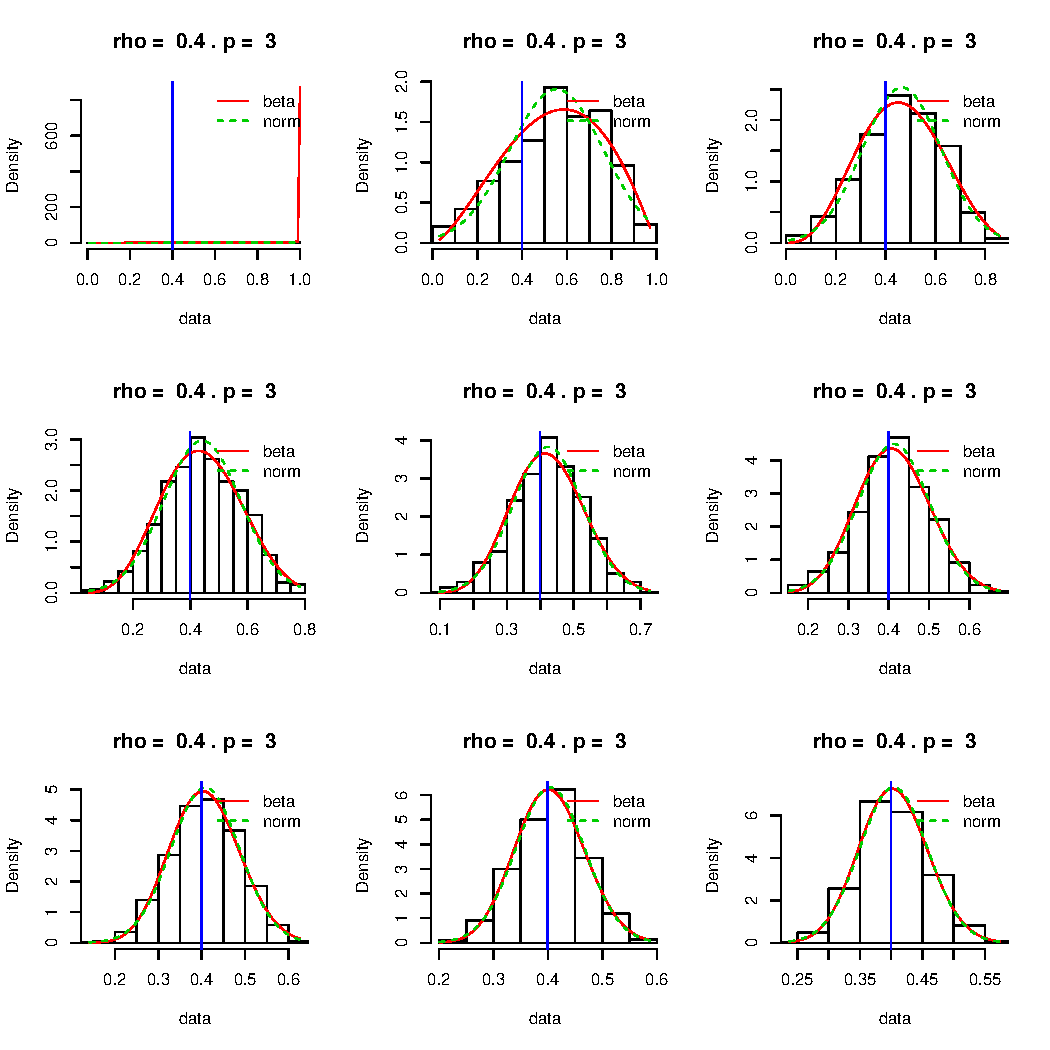
\includegraphics{2016_w09_files/figure-latex/unnamed-chunk-15-5.pdf}
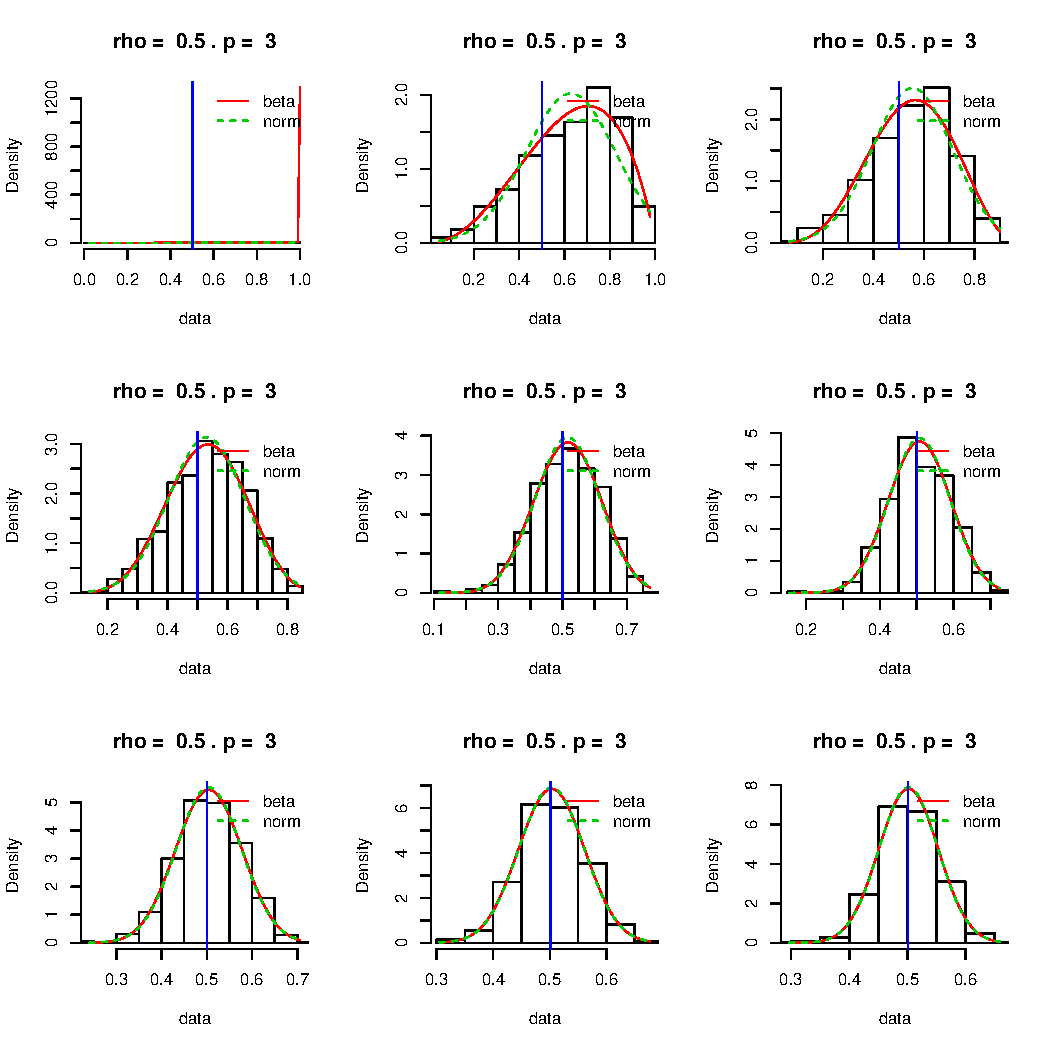
\includegraphics{2016_w09_files/figure-latex/unnamed-chunk-15-6.pdf}
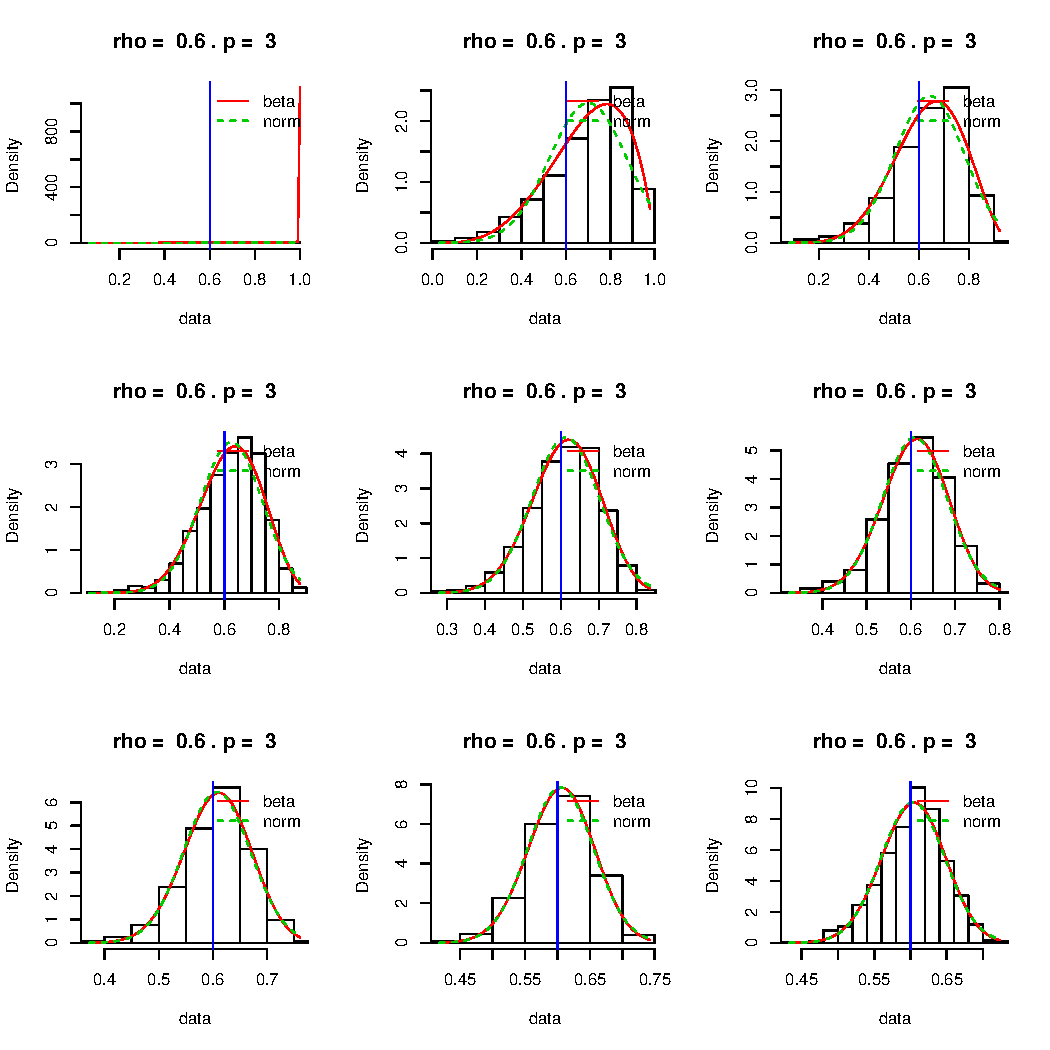
\includegraphics{2016_w09_files/figure-latex/unnamed-chunk-15-7.pdf}
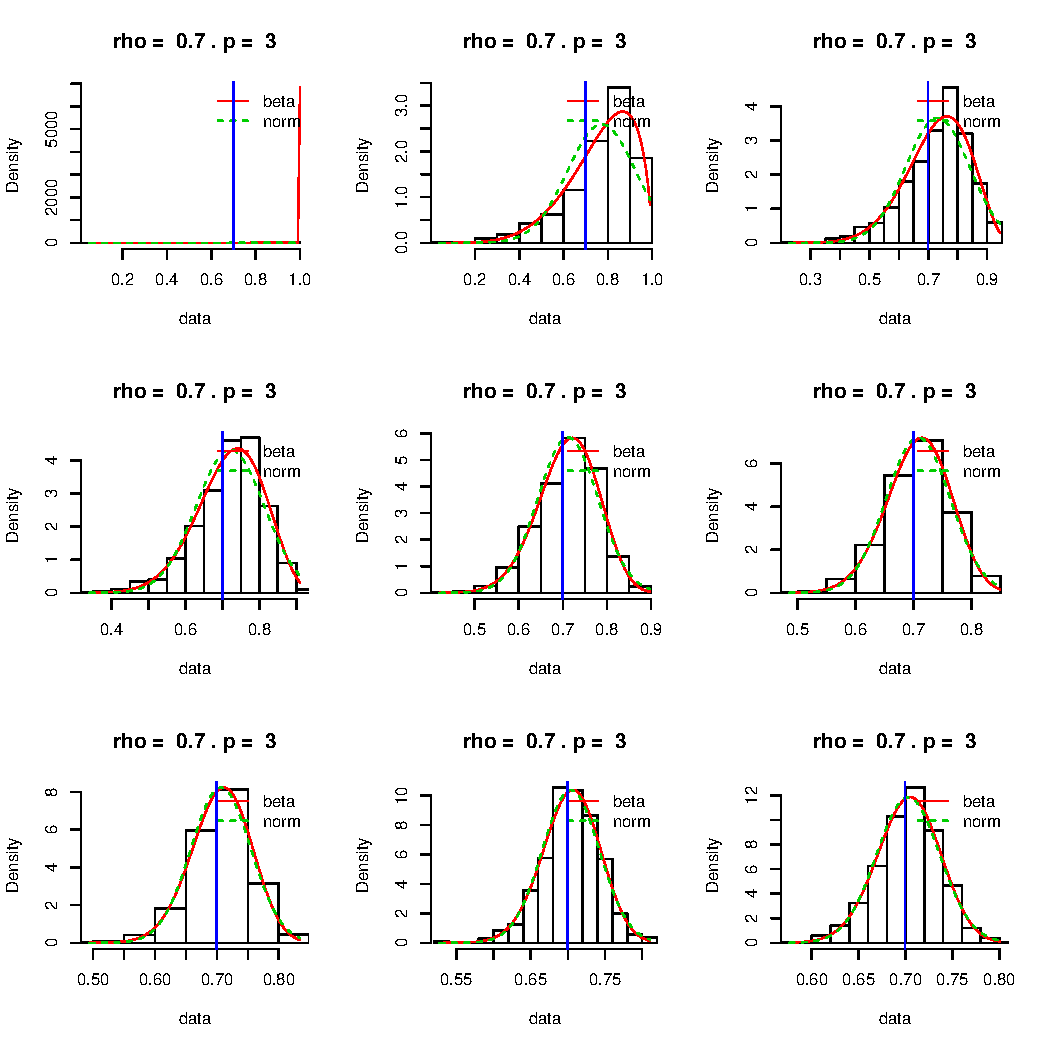
\includegraphics{2016_w09_files/figure-latex/unnamed-chunk-15-8.pdf}
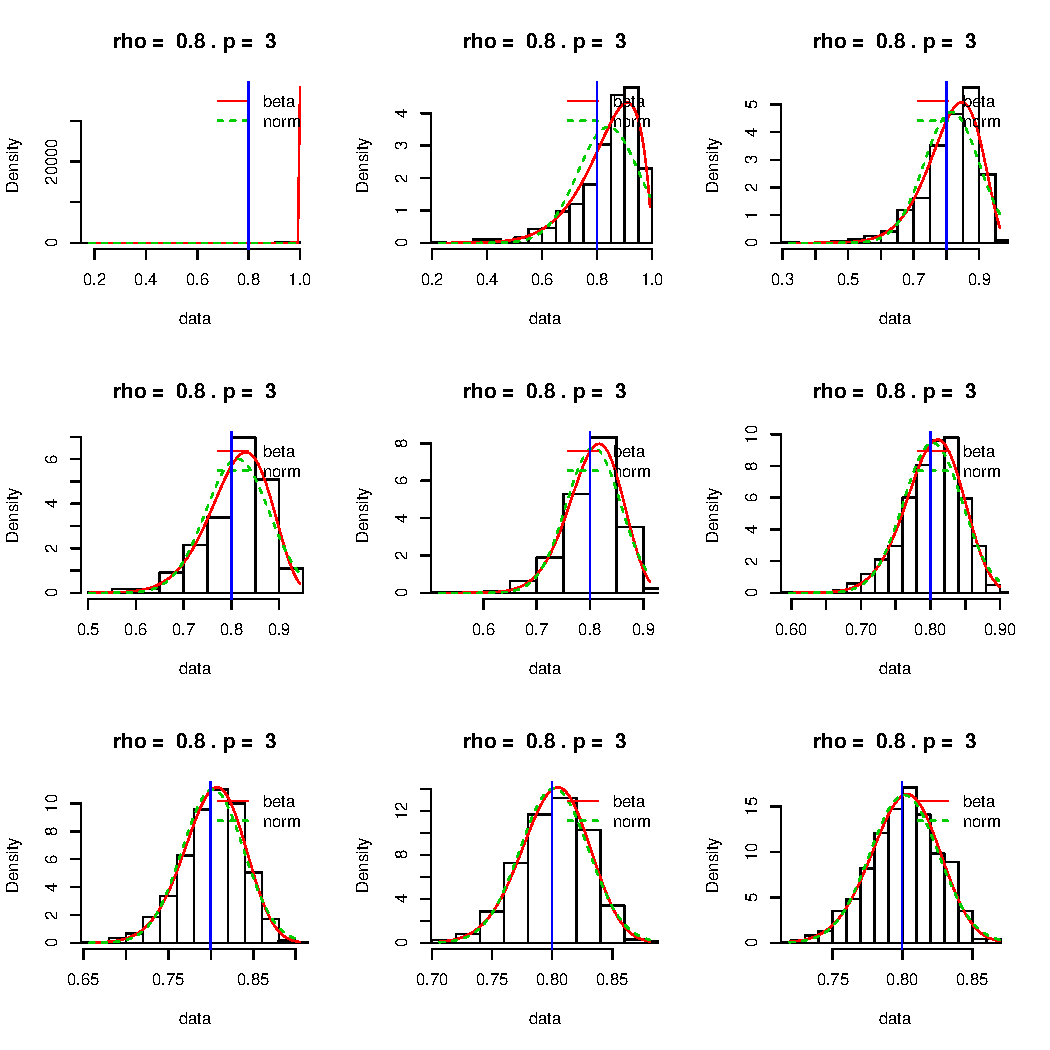
\includegraphics{2016_w09_files/figure-latex/unnamed-chunk-15-9.pdf}
\includegraphics{2016_w09_files/figure-latex/unnamed-chunk-15-10.pdf}

\subsubsection{\texorpdfstring{\(p > 3\)}{p \textgreater{} 3}}\label{p-3-1}

När jag provar med större p får jag konvergensproblem av \texttt{optim}
enl kod 100 på \texttt{?mle}

Sedan är det förstås viktigt att också titta på CDF, QQ och PP-plottar
där QQ illustrerar lack of fit i svansarna och PP i mitten
(Delignette-muller and Dutang 2015). Funktionen \texttt{gofstat} kan
också användas för att få fram en del teoretiska värden som beskriver
goodness of fit. I så fall kan Anderson-Darling statistican vara bra att
undersöka då den ger vikt till svansarna. Men finns också brister.
AIC/BIC kan rekommenderas vid jämförelse mellan olika fördelningar.

Går också lätt att få konfidensnitervall för paremeterskattningarna gm
bootstrap via funktionne \texttt{bootdist}.

\subsection{Läsning av (Kohl and Ruckdeschel
2010)}\label{lasning-av-distrmod}

Väldigt lätt att t ex plotta en ickecenrtal betafördelning (här med
defaultparametervärden).

\begin{Shaded}
\begin{Highlighting}[]
\KeywordTok{library}\NormalTok{(distrMod)}
\NormalTok{B <-}\StringTok{ }\KeywordTok{Beta}\NormalTok{()}
\KeywordTok{plot}\NormalTok{(B)}
\end{Highlighting}
\end{Shaded}

\includegraphics{2016_w09_files/figure-latex/unnamed-chunk-16-1.pdf}

Skattningar sker via \texttt{MCEstimator} (\texttt{MLEstimator}) men för
detta krävs en familj att skatta emot. Det fnins en \texttt{BetaFamily}
men den omfattar inte ickecentral beta. Man kan defeniera en egen familj
via \texttt{L2ParamFamily} (se t ex källkoden för \texttt{BetaFamily}).
Dock är jag osäker på argumentet \texttt{L2deriv.fct}. Det ska bestå av
tre funktioner i en lista där varje funktion av \(x\) beskriver
vänsterledet i \(\frac{\partial \alpha}{\partial f} \ln{\hat{l}} = 0\)
där \(f\) är fördelningsfunktionen för beta, dvs ett uttryck för att
finna maximum likelihood-estimatet (digamma = derivatan av
gammafördelningen). Dessa funktioner går att beräkna analytiskt för
betafördelningen men går det för ickecentral beta? Fördelningsfunktionen
finns här:
\url{https://en.wikipedia.org/wiki/Noncentral_beta_distribution\#Probability_density_function}

Om vi sedan deriverar Betafunktionen fnins det uttrycket här:
\url{https://en.wikipedia.org/wiki/Beta_function\#Derivatives}

\section{2016-03-03}\label{section-3}

Jobbar hemifrån med att läsa.

\subsection{Läsning av (Kowalski 1972)}\label{lasning-av-kowalski1972}

Behandlar sampling från icke bivariat normalfördelning.Jämförr (ej
\(r^2\)) mot normalfördelning.Undersöker tidigare konflikter om
robusthet hos \(r\). Nämner att Fisher redan 1915 utvecklade en exakt
formel för samplingsfördelningen av \(r\) då underliggande data bivariat
normalfördelad.

\[f_N(r|\rho) = \frac{2^{N-3}(1-\rho^2)^{(N-1)/2}(1-r^2)^{(N-4)/2}}{\Gamma(N-2)\pi} \sum_{j = 0}^\infty \frac{(2r)^j}{j!}\Gamma^2[(N+j-1)/2]\]

och då \(\rho = 0\):

\[f_N(r|\rho=0) = \frac{\Gamma[(N-1)/2]}{\Gamma[(N-2)/2]\sqrt{\pi}}(1-r^2)^{(N-4)/2} \]

Tycker dok inte det är så tydligt att just (Fisher and Fisher 1915)
anger detta men är förmodligen bara lost in notation. I vilket fall som
helst alltså oändlig serie och bara för \(r\), ej \(r^2\). Detta anges
också av (Hotelling 1953) men det är först i (Hogben 1968) som
resultatet utvecklas för \(r^2\).

Redan åren efter (Fisher and Fisher 1915) gjordes en del studierav
fördelningens robusthet. Ibland baserat på teoretiska formler, ibland på
monte carlo-simuleringar. Åsikterna gick brett isär huruvida
fördelningen var robust eller inte. Detta gås igenom med referernser
till olika artiklar i avs 2.1. Observera dock att jämförelserna endast
avser normalfördelning och ej beta. Här finns alltså kanske fortfarande
ett utrymme för att jämföra mot vanlig betafördelning. De flesata dock
överrens om att svårigheter uppstår främst då \(|\rho| \lesssim 1\).
Lättast att finna likheterna då \(\rho \approx 0\).

\textbf{Alltså:} de flesta är överrens om att \(r|\rho=0 \sim N\) men
\(r|\rho \neq 0 \nsim N\). Skulle motsv att \(r^2|\rho=0 \sim \chi^2_1\)

Förklarar att tidiagre resultat som pekat påicke robust
fördelningsantagande i själva verket kan härledas till att man på den
tiden saknade hjkälpmedel (datorer) för att kunna beräkna saker
ordentligt. Nu vill han kolla på detta igen med hjälp av modern teknik.
I slutet av 1960-talet undersöktes också approximationer mha
fouriertransformer. Här skapas en sådan formel (men den är fortfarande
ganska icke intuitiv) för att kunna användas vid fortsatta studier.

Resultatet visar att fördelningen alls icke var så robust som man
tidigare antagit. UNdersökning görs med flera olika typer av data från
olika fördelningar (mixade normal, exponential etc). Motsäger också t ex
tidigarte studie som påstått sig funnit robust resultat i intervallet
\(\rho \in [.1, .8], n = 5\). KOnstateras också att andra
korrelationsmått såsom kendals och Spearman är att föredra i en del fall
(vi har ju förstås inte motsvarande situation hos oss då vi betraktar
\(r^2\)).

\subsection{Läsnig av (Barrett 1974)}\label{lasnig-av-barrett1974}

Handlar nu äntligen om \(r^2\). Väldigt kort artikel, 2 sidor med endast
4 referenser (innehåller f.ö. en annons \ldots{} för en statistikkurs).

Kritiserar att man tar \(R^2 = r^2\) som enda mått för regressionens
giltighet. Föreslår att man också använder konfidensintervall etc för
att undersöka goodnes-of-fit etc. Menar att många övertolkar nyttan av
koefficienten och ger den mening som den egentligen saknar.

Menar att en linjär regressionsmodell med brant lutning kan ha högt
\(r^2\) utan att man för den sakens skullfår bättre prediktioner än för
en modell med lägre \(r^2\) men mindre brant lutning. Ställer också upp
en tabell över hur \(r^2\) ökar med ökad lutning (rotation av data). Går
mot 1 då vinkeln på slop går mot 90 grader.

Innehåller inget som är av direkt relevansjust nu men en lite intressant
side note.

\subsection{Läsning av (Claudy 1978)}\label{lasning-av-claudy1978}

Behandlar studie av empiriskt utvecklad ekvation för multiple regression
coefficient. Nämnar avvägningsproblem med stickprovsstorlek i
förhållande till validering för cross-validation. Beskriver att
regression utvecklades för designade experiment med fixt X och att det
inte riktigt stämmer med förutsättningarna inomsurvey eller psykologisk
forskning. I dessa fall måste man räkna med sampling och measurement
errors även på de oberoende parametrarna. Nämner att det också finns
metoder att hantera då \(x\) är stokastisk variabel men att formler etc
för detta är så komplexa att de sällan används (kallas Random-X model
istf Fixed-X model).

\textbf{OBS!!!} Här står att:

\begin{quote}
Application of estimatiojn procedures based on the Fixed -X model to
Random-X data causes an over-fitting of the regression surface to the
available data. The regression surface is fitted to the sample specific
error varianceas well as to the systematic trends of the population.
This over-fitting, or error-fitting, results in the sample multiple
correlation coefficient overestimating the actual population multiple
correlation.
\end{quote}

Detta är kanske vad vi ser då vi överskattar \(r^2\) med \(p> 1\)? Dvs
förklaring till att vår bias inte bara är additiv utan dessutom ökar
lite mer än så för varje ökning av \(p\)?

Detta är bakgrunden till adjusted \(R^2\) enl (Larson 1931) (tillskrevs
B Smith), sedan modifierad till dagens form av (Wherry 1931). Men som ju
senare visade sig vara biased och ist leda till underskattning av
\(\rho\) (nämner också nya versionen av (Olkin and Pratt 1958) etc).
Även senare approximationer av dessa diskuteras.

Nämner också att cross-validation tenderar underskatta \(\rho\) (se
{[}5{]}).

Nämner speciella formler för skattning av \(\rho\) vid korsvalidering!
(Man hade ännu inte 10-fold etc men åtm 2-fold). Intressant! Finns för
både fixed och random x.

Visar fig 1 som påminner om våra liknande resultat med jämförelse av
\(\rho, r\) där \(r\) överskattar \(\rho\) men närmar sig assymptotiskt.
Dock med crass-validerings-\(r/\rho\) istf adjusted \(R^2\) som vi hade.

Gör en simuleringsstudie som tycks väldigt lik vår. Använder olika typer
av fördelningar, interkorrelationsmatris och antal oberoende variabler
(max 5). Dock populationer med 500 fall istf 1e6. Endast 400 samples
totalt från ursprungspopulationen, 100 av varje storlek 20, 40, 80 och
160.

Man antar här att 500 är tillräckligt för att approximera oändligheten
(var det Fisher eller t om Pearson som tyckte man skulle ha åtm 1000 i
stickprovet.)?

\textbf{OBS!} Här tillåter man alltså en variation av
correlationsmatrisen som kan vara intressant och som kanske kan
undersköas även hos oss?

Resultat visar att korsvalidering ger bäst resultat. På den tiden
ifrågasatte man dock om det var värt den extra tiden och kraften att
tilläpa korsvalidering. Ett argument som antagligen är mindre relevant
idag.

Föreslår (på empirisk grund) en kompromiss som dels ska var lika unbias
som vid korsvalidering men som inte ska kräva just korsvalidering då det
anses för krångligt. Formeln funkar bra för större stickprov men för upp
till 20 är änd¨korsvalidering bättre.

\[\hat{\rho} = \sqrt{1 - \frac{(N-4)(1-r^2)}{N-n-1}(1 + \frac{2(1-r^2)}{N-n+1})}\]

Dock saknas en parentes i formeln men jag tror det är så den ska se ut.

Föreslår att denna formel används vid tillräcklig stickprovsstorlek men
kan inte erbjuda ngn teoretisk motivering.

Påminner docj att (Skidmore and Thompson 2011) ej fann denna formel
överlägsen utan istället håller fast vid (Olkin and Pratt 1958).
Påminner f.ö. om intressant uppställning i tabell 3 (Olkin and Pratt
1958) som också jämför för \(r^2=.01\).

Noteras f.ö. att studien sponsrats av NASA avseende datorresurser :-)

\subsection{Läsning av (Konishi 1978)}\label{lasning-av-konishi1978}

Föreslår approximativ fördelning för sample correlation coefficient, dvs
\(r\), inte \(r^2\) (från Hiroshima!).

Avser endast då grunddata bivariat normalfördelad. Sägs vara bättre än
tidigare försök och ganska enkel. Tycker dok ändå att den ges av en
hyfsat komplex formel. Kan heller inte bevisas teoretiskt att detta är
den bästa lösningen. Involverar Fishers z-transform.

\subsection{Läsning av en blogg}\label{lasning-av-en-blogg}

Enligt Dave Giles gäller att
\url{http://davegiles.blogspot.se/2013/10/more-on-distribution-of-r-squared.html}

\[r^2|\rho = 0 \sim Beta(\frac{k-1}{2}, \frac{n-k}{2})\] där \$k = \$
vårt \(p+1\) och \$n = \$ stickprovsstorlek. Nämner dock bara i
förbigående (som svar på en kommentar att det blir ickecentral beta då
\(\rho \neq 0\)).

Samme Gilers noterar också
(\url{http://davegiles.blogspot.se/2013/05/good-old-r-squared.html})
\textgreater{} Whenever the bias of R2 is noticeable, its standard
deviation is several times larger than this bias.

\begin{quote}
First, the coefficient of determination is a sample statistic, and as
such it is a random variable with a sampling distribution. Second, the
form of this sampling distribution depends on the X data, and on the
unknown beta and sigma parameters. Third, this sampling distribution
gets distorted if the regression errors are autocorrelated. Finally,
even if we have a very large sample of data, R2 converges in probability
to a value less than one, regardless of the data values or the values of
the unknown parameters.
\end{quote}

\subsection{Läsning av (Alam 1979)}\label{lasning-av-alam1979}

Denna artikel finns publicerad men kostar då pengar. Den version jag
läst tycks vara digitalisering av mikrofilm och originalet skrivet på
skrivmaskin.Därmed lite svårläst.

Behandlar \(r\), ej \(r^2\). Begr till bivariat normalfördelning.

Ärligt talat en inte så värst angenäm läsning. Teoretiskt förslag som
jsg tvivlar på blivit så uppmärksammat.

\subsection{Läsning av (Huberty and Mourad
1980)}\label{lasning-av-huberty1980}

Behandlar just multiple correlation och \(R^2\)! Dock främst en
jämförelse mellan sedan tidigare kända formler såsom (Ezekei 1929) och
(Olkin and Pratt 1958).

Nämner att för \(\rho = 0\) gäller:

\[E[R^2] = \frac{p}{N-1}\]

Käns som att denn artikel gör mkt av det vi vill göra. Välskriven och
pedagogisk. Tillämpas på verklig fata (ej simulerat).

Man skiljer på modeller för att förstå samband eller för predektion på
sätt som jag inte riktigt sett tidigare.

\textbf{OBS!} Här noteras också (vilket jag själv tidiagre också nämnt)
att (Ezekei 1929) först använde \(N\) där han senare använde \(N - 1\).

Nämner jack-knife som alternativ till adjusted \(R^2\).

Använder lånade data set med betyg och olika elevdata som predektorer.
Två dataset varav första med \(p = 9\).

Stickprovsstorlek på 50.

SKriver att om \(N/p>20\) så kan ``shrinkage'' negligeras.

Endast tio upprepade försök per stickprovsstorlek.

Tra olika \(\rho^2\), samtliga mellan 0,3 och 0,4.

Från dessa stickprov mättes:

\begin{itemize}
\tightlist
\item
  precision via standardavvikelse av avvikelse mellan \(\rho^2\) och
  \(\hat{rho}\).
\item
  accuracy via dess medelvärde.
\end{itemize}

Slutsatser: (Ezekei 1929) och (Olkin and Pratt 1958) hyfsat lika
resultat. Mer bias för högre \(p\). Biasen var väldigt liten (notera n =
50) och saknade signifikant avvikelse från 0. Alla adjusted \(R^2\) kan
bedömas likvärdiga.

Noterar att adjusted \(R^2\) kan bli negativt men att detta motsvarar en
riktigt dålig passning (väldigt litet \(R^2\) och \(n\)).

\subsection{Läsning av (Wood 1986)}\label{lasning-av-wood1986}

Kritiserar generaliseringen att kvadrera \(\rho\) beräknat för
korrelation för att få ett värde som motsvarar \(R^2\) vid regression.
Säger alltså inte emot att coefficient of determination beräknas så men
menar att man inte kan alltid kan tolka \(\rho^2\) som sådan koefficient
ifall det inte var syftet från början. Detta eftersom korrelation
baseras på stokastiskt X medan regression baseras på fixt X.Hänvisar
också til (Warren 1971) ang detta.

Wood kallar dessa felaktiga resonemang för ``vulgarised knowledge''.

\begin{quote}
``bias (for correlation) and precision (for regression) tend to work
against each other. One should determine which of correlation or
regression is appropriate to the problem and select the sampling method
accordingly
\end{quote}

Hela artikeln känns polemisk och lite ``von oben'' men kommunicerar å
andra sidan ganska klart sin ståndpunkt.

Argumenterar också för att korrelationsvärden inte ska tillmätas alltför
stort värde rakt av utan att man måste undersöka hela fördelningen
grafiskt. Detta kan förstås vara svårt vid publicering men det bör åtm
ske i explorativt syfte.

\subsection{Läsning av (Hawkins 1989)}\label{lasning-av-hawkins1989}

Väldigt kort. Handlar om Fisher z. Teoretisk, många formler. Kopierar
abstract:

\begin{quote}
A simple derivation of the asymptotic distribution of Fish- er's Z
statistic for general bivariate parent distributions F is obtained using
U-statistic theory. This method easily reveals that the asymptotic
variance of Z generally depends on the correlation \(\rho\) and on
certain moments of F. It also reveals the particular structure of F that
makes the asymptotic variance of Z independent of \(\rho\), and shows
that there are many distributions F with this property. The bivariate
normal is only one such F.
\end{quote}

Refererar till (Gayen 1951) som visade samma sak men då endast för
Edgeworth-fördelningar. Detta bevis gäller alla fördelningar med ändligt
fjärdemoment (kurtosis) men bara approximativt då
\(n \rightarrow \infty\)

\subsection{Läsning av (Nagelkerke
1991)}\label{lasning-av-nagelkerke1991}

Kort. 2 sidor och fgå referenser. Teoretisk.

Tar här för givet att coefficient of determination = multiple
correlation coefficient.

Beskriver generalisering som kan användas utanför linjär regression.
Baseras på maximum likelihood. Har egentligen introducerats redan
tidigare av bl a Cox et al. Beskriver många fina egenskaper men också
ett problem som dock går att överkomma.

\section*{Referenser}\label{referenser}
\addcontentsline{toc}{section}{Referenser}

\hypertarget{refs}{}
\hypertarget{ref-Alam1979}{}
Alam, Kursheed. 1979. ``Distribution of sample correlation
coefficients.'' \emph{Naval Research Logistics Quarterl} 26: 237--330.

\hypertarget{ref-Barrett1974}{}
Barrett, James P. 1974. ``The Coefficient of Determination---Some
Limitations.'' \emph{The American Statistician} 28 (1): 19--20.
doi:\href{https://doi.org/10.1080/00031305.1974.10479056}{10.1080/00031305.1974.10479056}.

\hypertarget{ref-Claudy1978}{}
Claudy, J. G. 1978. ``Multiple Regression and Validity Estimation in One
Sample.'' \emph{Applied Psychological Measurement} 2 (4): 595--607.
doi:\href{https://doi.org/10.1177/014662167800200414}{10.1177/014662167800200414}.

\hypertarget{ref-Cowden1952}{}
Cowden, Dudley J. 1952. ``The Multiple-Partial Correlation
Coefficient.'' \emph{Journal of the American Statistical Association} 47
(259): 442--56.
doi:\href{https://doi.org/10.1080/01621459.1952.10501183}{10.1080/01621459.1952.10501183}.

\hypertarget{ref-fitdistrplus}{}
Delignette-muller, Marie Laure, and Christophe Dutang. 2015.
``fitdistrplus : An R Package for Fitting Distributions.'' \emph{Journal
of Statistical Software} 64 (4): 1--34.
doi:\href{https://doi.org/10.18637/jss.v064.i04}{10.18637/jss.v064.i04}.

\hypertarget{ref-Ezekei1929}{}
Ezekei, Mordecai. 1929. ``The Application of the Theory of Error to
Multiple and Curvilinear Correlation.'' \emph{Journal of the American
Statistical Association} 24 (165): 99--104.

\hypertarget{ref-Fisher1915}{}
Fisher, R.a., and R.a. Fisher. 1915. ``Frequency distribution of the
values of the correlation coefficient in samples from an indefinitely
large population.'' \emph{Biometrika} 10 (4): 507--21.
doi:\href{https://doi.org/10.2307/2331838}{10.2307/2331838}.

\hypertarget{ref-Gayen1951}{}
Gayen, A. K. 1951. ``The Frequency Distribution of the Product-Moment
Correlation Coefficient in Random Samples of Any Size Drawn from
Non-Normal Universes.'' \emph{Biometrika} 38 (1/2): 219--47.

\hypertarget{ref-Hawkins1989}{}
Hawkins, D. 1989. ``Using U statistics to derive the asymptotic
distribution of Fisher's Z statistic.'' \emph{American Statistician} 43
(4): 235--37.
doi:\href{https://doi.org/10.2307/2685369}{10.2307/2685369}.

\hypertarget{ref-Hogben1968}{}
Hogben, David. 1968. ``The distribution of the sample correlation
coefficient with one variable fixed.'' \emph{Journal of Research of the
National Bureau of Standards, Section B: Mathematical Sciences} 72B (1):
33.
doi:\href{https://doi.org/10.6028/jres.072B.007}{10.6028/jres.072B.007}.

\hypertarget{ref-Hotelling1953}{}
Hotelling, Harold. 1953. ``New Light on the Correlation Coefficient and
its Transforms Author(s): Harold Hotelling.'' \emph{Journal of the Royal
Statistical Society. Series B (Methodological),} 15 (2): 296--193--232.

\hypertarget{ref-Huberty1980}{}
Huberty, Carl J, and Salah A Mourad. 1980. ``Estimation in multiple
correlation/prediction.'' \emph{Educational and Psychological
Measurement} 40: 101--12.

\hypertarget{ref-distrMod}{}
Kohl, Matthias, and Peter Ruckdeschel. 2010. ``R Package distrMod: S4
Classes and Methods for Probability Models.'' \emph{Journal of
Statistical Software} 35 (10): 1--27.
doi:\href{https://doi.org/10.1002/wics.10}{10.1002/wics.10}.

\hypertarget{ref-Konishi1978}{}
Konishi, Sandnori. 1978. ``An Approximation to the Distribution of the
Sample Correlation Coefficient.'' \emph{Biometrika} 65 (3): 654--56.

\hypertarget{ref-Kowalski1972}{}
Kowalski, Charles J. 1972. ``On the Effects of Non-Normality on the
Distribution of the Sample Product-Moment Correlation Coefficient.''
\emph{Journal of the Royal Statistical Society} 21 (1): 1--12.
doi:\href{https://doi.org/10.2307/2346598}{10.2307/2346598}.

\hypertarget{ref-Kymn1968}{}
Kymn, Kern O . 1968. ``The Distribution of the Sample Correlation
Coefficient Under the Null Hypothesis.'' \emph{Econometrica} 36 (1):
187--89.

\hypertarget{ref-Larson1931}{}
Larson, S C. 1931. ``The shrinkage of the coefficient of multiple
correlation.'' \emph{Journal of Educational Psychology} 22 (1): 45--55.
doi:\href{https://doi.org/10.1037/h0072400}{10.1037/h0072400}.

\hypertarget{ref-Nagelkerke1991}{}
Nagelkerke, N. J D. 1991. ``A note on a general definition of the
coefficient of determination.'' \emph{Biometrika} 78 (3): 691--92.
doi:\href{https://doi.org/10.1093/biomet/78.3.691}{10.1093/biomet/78.3.691}.

\hypertarget{ref-Nemes2009}{}
Nemes, Szilard, Junmei Miao Jonasson, Anna Genell, and Gunnar Steineck.
2009. ``Bias in odds ratios by logistic regression modelling and sample
size.'' \emph{BMC Medical Research Methodology} 9: 56.
doi:\href{https://doi.org/10.1186/1471-2288-9-56}{10.1186/1471-2288-9-56}.

\hypertarget{ref-Olkin1958}{}
Olkin, Ingram, and J.W. Pratt. 1958. ``Unbiased estimation of certain
correlation coefficients.'' \emph{The Annals of Mathematical Statistics}
29 (1): 201--11.
doi:\href{https://doi.org/10.2307/2237306}{10.2307/2237306}.

\hypertarget{ref-Park1964}{}
Park, John H Jr. 1964. ``Variations of the Non-central t and Beta
Distributions.'' \emph{The Annals of Mathematical Statistics} 35 (4):
1583--93.

\hypertarget{ref-Pearson1895}{}
Pearson, Karl. 1895. ``Note on Regression and Inheritance in the Case of
Two Parents.'' \emph{Proceedings of the Royal Society of London
(1854-1905)} 58: 240--42.
doi:\href{https://doi.org/10.1098/rspl.1895.0041}{10.1098/rspl.1895.0041}.

\hypertarget{ref-Pearson1896}{}
---------. 1896. ``Mathematical Contributions to the Theory of
Evolution. III. Regression, Heredity, and Panmixia.''
\emph{Philosophical Transactions of the Royal Society A} 187.

\hypertarget{ref-Skidmore2011}{}
Skidmore, Susan Troncoso, and Bruce Thompson. 2011. ``Choosing the Best
Correction Formula for the Pearson r 2 Effect Size.'' \emph{The Journal
of Experimental Education} 79 (3): 257--78.
doi:\href{https://doi.org/10.1080/00220973.2010.484437}{10.1080/00220973.2010.484437}.

\hypertarget{ref-Warren1971}{}
Warren, W. G. 1971. ``Correlation or Regression: Bias or Precision.''
\emph{Applied Statistics} 20 (2): 148.
doi:\href{https://doi.org/10.2307/2346463}{10.2307/2346463}.

\hypertarget{ref-Wherry1931}{}
Wherry, R. 1931. ``A new formula for predicting the shrinkage of the
coefficient of multiple correlation.'' \emph{The Annals of Mathematical
Statistics} 2 (4): 440--57.
\url{http://www.jstor.org/stable/2957681$/backslash$npapers2://publication/uuid/F3D4916B-BB98-4094-A459-DF4387AC9610}.

\hypertarget{ref-Wood1986}{}
Wood, Robert. 1986. ``Think Before you Square Correlations---or do
anything with them.'' \emph{British Educational Research Journal} 12
(3): 249--55.
doi:\href{https://doi.org/10.1080/0141192860120303}{10.1080/0141192860120303}.

\end{document}
